\documentclass[]{elsarticle} %review=doublespace preprint=single 5p=2 column
%%% Begin My package additions %%%%%%%%%%%%%%%%%%%
\usepackage[hyphens]{url}

  \journal{Some Journal} % Sets Journal name


\usepackage{lineno} % add
  \linenumbers % turns line numbering on

\usepackage{graphicx}
%%%%%%%%%%%%%%%% end my additions to header

\usepackage[T1]{fontenc}
\usepackage{lmodern}
\usepackage{amssymb,amsmath}
\usepackage{ifxetex,ifluatex}
\usepackage{fixltx2e} % provides \textsubscript
% use upquote if available, for straight quotes in verbatim environments
\IfFileExists{upquote.sty}{\usepackage{upquote}}{}
\ifnum 0\ifxetex 1\fi\ifluatex 1\fi=0 % if pdftex
  \usepackage[utf8]{inputenc}
\else % if luatex or xelatex
  \usepackage{fontspec}
  \ifxetex
    \usepackage{xltxtra,xunicode}
  \fi
  \defaultfontfeatures{Mapping=tex-text,Scale=MatchLowercase}
  \newcommand{\euro}{€}
\fi
% use microtype if available
\IfFileExists{microtype.sty}{\usepackage{microtype}}{}
\bibliographystyle{elsarticle-harv}
\ifxetex
  \usepackage[setpagesize=false, % page size defined by xetex
              unicode=false, % unicode breaks when used with xetex
              xetex]{hyperref}
\else
  \usepackage[unicode=true]{hyperref}
\fi
\hypersetup{breaklinks=true,
            bookmarks=true,
            pdfauthor={},
            pdftitle={Introducing spatial availability, a singly-constrained measure of competitive accessibility},
            colorlinks=false,
            urlcolor=blue,
            linkcolor=magenta,
            pdfborder={0 0 0}}
\urlstyle{same}  % don't use monospace font for urls

\setcounter{secnumdepth}{5}
% Pandoc toggle for numbering sections (defaults to be off)


% tightlist command for lists without linebreak
\providecommand{\tightlist}{%
  \setlength{\itemsep}{0pt}\setlength{\parskip}{0pt}}


% Pandoc citation processing
\newlength{\cslhangindent}
\setlength{\cslhangindent}{1.5em}
\newlength{\csllabelwidth}
\setlength{\csllabelwidth}{3em}
\newlength{\cslentryspacingunit} % times entry-spacing
\setlength{\cslentryspacingunit}{\parskip}
% for Pandoc 2.8 to 2.10.1
\newenvironment{cslreferences}%
  {}%
  {\par}
% For Pandoc 2.11+
\newenvironment{CSLReferences}[2] % #1 hanging-ident, #2 entry spacing
 {% don't indent paragraphs
  \setlength{\parindent}{0pt}
  % turn on hanging indent if param 1 is 1
  \ifodd #1
  \let\oldpar\par
  \def\par{\hangindent=\cslhangindent\oldpar}
  \fi
  % set entry spacing
  \setlength{\parskip}{#2\cslentryspacingunit}
 }%
 {}
\usepackage{calc}
\newcommand{\CSLBlock}[1]{#1\hfill\break}
\newcommand{\CSLLeftMargin}[1]{\parbox[t]{\csllabelwidth}{#1}}
\newcommand{\CSLRightInline}[1]{\parbox[t]{\linewidth - \csllabelwidth}{#1}\break}
\newcommand{\CSLIndent}[1]{\hspace{\cslhangindent}#1}

\usepackage[font=small,skip=0pt]{caption}
\usepackage{booktabs}
\usepackage{longtable}
\usepackage{array}
\usepackage{multirow}
\usepackage{wrapfig}
\usepackage{float}
\usepackage{colortbl}
\usepackage{pdflscape}
\usepackage{tabu}
\usepackage{threeparttable}
\usepackage{threeparttablex}
\usepackage[normalem]{ulem}
\usepackage{makecell}
\usepackage{xcolor}
\usepackage{caption}
\usepackage{graphicx}
\usepackage{siunitx}
\usepackage{hhline}
\usepackage{calc}
\usepackage{tabularx}
\usepackage{adjustbox}
\usepackage{hyperref}



\begin{document}


\begin{frontmatter}

  \title{Introducing spatial availability, a singly-constrained measure
of competitive accessibility}
      
  \begin{abstract}
  Accessibility indicators are widely used in transportation, urban, and
  healthcare planning, among many other applications. These measures are
  weighted sums of reachable opportunities from a given origin
  conditional on the cost of movement, and are estimates of the
  potential for spatial interaction. Over time, various proposals have
  been forwarded to improve their interpretability, mainly by
  introducing competition. In this paper, we demonstrate how a widely
  used measure of accessibility with congestion fails to properly match
  the opportunity-seeking population. We then propose an alternative
  formulation of accessibility with competition, a measure we call
  \emph{spatial availability}. This measure results from using balancing
  factors that are equivalent to imposing a single constraint on
  conventional gravity-based accessibility. Further, we demonstrate how
  Two-Stage Floating Catchment Area (2SFCA) methods can be
  reconceptualized as singly-constrained accessibility. To illustrate
  the application of spatial availability and compare it to other
  relevant measures, we use data from the 2016 Transportation Tomorrow
  Survey of the Greater Golden Horseshoe area in southern Ontario,
  Canada.
  \end{abstract}
  
 \end{frontmatter}

\newpage

\hypertarget{sec:introduction}{%
\section{Introduction}\label{sec:introduction}}

The concept of accessibility in transportation studies derives its
appeal from the combination of the spatial distribution of opportunities
and the cost of reaching them (Handy and Niemeier, 1997; Hansen, 1959).
Accessibility analysis is employed in transportation, geography, public
health, and many other areas, with the number of applications growing
(Shi et al., 2020), especially as mobility-based planning is
de-emphasized in favor of access-oriented planning (Deboosere et al.,
2018; Handy, 2020; Proffitt et al., 2017; Yan, 2021).

Accessibility analysis stems from the foundational works of Harris
(1954) and Hansen (1959). From these seminal efforts, many accessibility
measures have been derived, particularly after the influential work of
Wilson (1971) on spatial interaction\footnote{Utility-based measures
  derive from a very different theoretical framework, random utility
  maximization}. Of these, gravity-type accessibility is arguably the
most common; since its introduction in the literature, it has been
widely adopted in numerous forms (Arranz-López et al., 2019; Cervero et
al., 2002; Geurs and van Wee, 2004; Levinson, 1998; Paez, 2004).
Hanson-type accessibility indicators are essentially weighted sums of
opportunities, with the weights given by an impedance function that
depends on the cost of movement, and thus measure the \emph{intensity of
the possibility of interaction} (Hansen, 1959). This type of
accessibility analysis offers a powerful tool to study the intersection
between urban structure and transportation infrastructure (Handy and
Niemeier, 1997).

Despite their usefulness, the interpretability of Hansen-type
accessibility measures can be challenging (Geurs and van Wee, 2004;
Miller, 2018). Since they aggregate opportunities, the results are
sensitive to the size of the region of interest (e.g., a large city has
more jobs than a smaller city). As a consequence, raw outputs are not
necessarily comparable across study areas (Allen and Farber, 2019). This
limitation becomes evident when surveying studies that implement this
type of analysis. For example, Páez et al. (2010) (in Montreal) and
Campbell et al. (2019) (in Nairobi) report accessibility as the number
of health care facilities that can potentially be reached from origins.
But what does it mean for a zone to have accessibility to less than 100
facilities in each of these two cities, with their different populations
and number of facilities? For that matter, what does it mean for a zone
to have accessibility to more than 700 facilities in Montreal, besides
being ``accessibility rich''? As another example, Bocarejo S. and Oviedo
H. (2012) (in Bogota), El-Geneidy et al. (2016) (in Montreal), and Jiang
and Levinson (2016) (in Beijing) report accessibility as numbers of
jobs, with accessibility values often in the hundreds of thousands, and
even exceeding one million jobs for some zones in Beijing and Montreal.
As indicators of urban structure, these measures are informative, but
the meaning of one million accessible jobs is harder to pin down: how
many jobs must any single person have access to? Clearly, the answer to
this question depends on how many people demand jobs.

The interpretability of Hansen-type accessibility has been discussed in
numerous studies, including recently by Hu and Downs (2019), Kelobonye
et al. (2020), and in greater depth by Merlin and Hu (2017). As hinted
above, the limitations in interpretability are frequently caused by
ignoring competition - without competition, each opportunity is assumed
to be equally available to every single opportunity-seeking individual
that can reach it (Kelobonye et al., 2020; Paez et al., 2019; Shen,
1998). This assumption is appropriate when the opportunity of interest
is non-exclusive, that is, if use by one unit of population does not
preclude use by another. For instance, national parks with abundant
space are seldom used to full capacity, so the presence of some
population does not exclude use by others. When it comes to exclusive
opportunities, or when operations may be affected by congestion, the
solution has been to account for competition. Several efforts exist that
do so. In our reckoning, the first such approach was proposed by Weibull
(1976), whereby the distance decay of the supply of employment and the
demand for employment (by workers) were formulated under so-called
axiomatic assumptions. This approach was then applied by Joseph and
Bantock (1984) in the context of healthcare, to quantify the
availability of general practitioners in Canada. About two decades
later, Shen (1998) independently re-discovered Weibull's (1976) formula
(see footnote (7) in Shen, 1998) and deconstructed it to consider
accessibility for different modes. These advances were subsequently
popularized as the family of Two-Stage Floating Catchment area (2SFCA)
methods (Luo and Wang, 2003) that have found widespread adoption in
healthcare, education, and food systems (B. Y. Chen et al., 2020; Chen,
2019; Z. Chen et al., 2020; Yang et al., 2006; Ye et al., 2018).

An important development contained in Shen's work is a proof that the
population-weighted sum of the accessibility measure with competition
equates to the number of opportunities available (footnote (7) and
Appendix A in Shen, 1998). This demonstration gives the impression that
Shen-type accessibility allocates \emph{all} opportunities to the
origins, however to the authors' knowledge, it has not interpreted by
literature in this way. For instance, Hu (2014), Merlin and Hu (2017),
and Tao et al. (2020) all use Shen-type accessibility to calculate job
access but report values as `competitive accessibility scores' or simply
`job accessibility'. These works do not explicitly recognize that jobs
that are assigned to each origin are in fact a proportion of \emph{all}
the opportunities in the system. This recognition, we argue, is critical
to interpreting the meaning of the final result. Thus, in this paper we
intend to revisit accessibility with competition within the context of
disentangling how opportunities are allocated. We first argue that
Shen's competitive accessibility misleadingly refers to the the total
zonal population to equal the travel-cost discounted opportunity-seeking
population. This equivocation, we believe, results in a ambigious
interpretation of what Shen-type accessibility represents as the
allocation of opportunities to population is masked by the results
presenting as rates (i.e., opportunities per capita). We then propose an
alternative formulation of accessibility that incorporates competition
by adopting a proportional allocation mechanism; we name this measure
\emph{spatial availability}. The use of balancing factors for
proportional allocation is akin to imposing a single constraint on the
accessibility indicator, in the spirit of Wilson's (1971) spatial
interaction model.

In this way, the aim of the paper is three-fold:

\begin{itemize}
\item
  First, we aim to demonstrate that Shen-type (and thus Weibull (1976)
  accessibility and the popular 2SFCA methods) produce equivocal
  estimates of opportunities allocated as the result is presented as a
  rate (i.e., opportunities per capita);
\item
  Second, we introduce a new measure, \emph{spatial availability}, which
  we submit is a more interpretable alternative to Shen-type
  accessibility, since opportunities in the system are preserved and
  proportionally allocated to the population; and
\item
  Third, we show how Shen-type accessibility (and 2SFCA methods) can be
  seen as measures of singly-constrained accessibility.
\end{itemize}

Discussion is supported by the use of the small synthetic example of
Shen (1998) and empirical data drawn from the 2016 Transportation
Tomorrow Survey of the Greater Toronto and Hamilton Area in Ontario,
Canada. In the spirit of openness of research in the spatial sciences
(Brunsdon and Comber, 2021; Páez, 2021) this paper has a companion open
data product (Arribas-Bel et al., 2021), and all code is available for
replicability and reproducibility purposes.

\hypertarget{background}{%
\section{Accessibility measures revisited}\label{background}}

In this section we revisit Hansen-type and Shen-type accessibility
indicators. We adopt the convention of using a capital letter for
absolute values (number of opportunities) and lower case for rates
(opportunities per capita).

\hypertarget{hansen-type-accessibility}{%
\subsection{Hansen-type accessibility}\label{hansen-type-accessibility}}

Hansen-type accessibility measures follow the general formulation shown
in Equation (\ref{eq:conventional-accessibility}):

\begin{equation}
\label{eq:conventional-accessibility}
S_i = \sum_{j=1}^JO_j \cdot f(c_{ij})
\end{equation}

\noindent where:

\begin{itemize}
\tightlist
\item
  \(c_{ij}\) is a measure of the cost of moving between \(i\) and \(j\).
\item
  \(f(\cdot)\) is an impedance function of \(c_{ij}\); it can take the
  form of any monotonically decreasing function chosen based on positive
  or normative criteria (Paez et al., 2012).
\item
  \(i\) is a set of origin locations (\(i = 1,\cdots,N\)).
\item
  \(j\) is a set of destination locations (\(j = 1,\cdots,J\)).
\item
  \(O_j\) is the number of opportunities at location \(j\);
  \(O = \sum_{j=1}^J O_j\) is the total supply of opportunities in the
  study region.
\item
  \(S\) is Hansen-type accessibility as weighted sum of opportunities.
\end{itemize}

As formally defined, accessibility \(S_i\) is the sum of opportunities
that can be reached from location \(i\), weighted down by an impedance
function of the cost of travel \(c_{ij}\). Summing the opportunities in
the neighborhood of \(i\) provides estimates of the number of
opportunities that can \emph{potentially} be reached from \(i\). Several
variants of this method result from using a variety of impedance
functions; for example, cumulative opportunities measures are obtained
when \(f(\cdot)\) is a binary or indicator function (e.g., El-Geneidy et
al., 2016; Geurs and van Wee, 2004; Qi et al., 2018; Rosik et al.,
2021). Other measures use impedance functions modeled after any
monotonically decreasing function (e.g., Gaussian, inverse power,
negative exponential, or log-normal, among others, see, \emph{inter
alia}, Kwan, 1998; Li et al., 2020; Reggiani et al., 2011; Vale and
Pereira, 2017). In practice, accessibility measures with different
impedance functions tend to be highly correlated (Higgins, 2019; Kwan,
1998; Santana Palacios and El-geneidy, 2022).

Gravity-based accessibility has been shown to be an excellent indicator
of the intersection between spatially distributed opportunities and
transportation infrastructure (Kwan, 1998; Reggiani et al., 2011; Shi et
al., 2020). However, beyond enabling comparisons of relative values they
are not highly interpretable on their own (Miller, 2018). To address the
issue or interpretability, previous research has aimed to index and
normalize values on a per demand-population basis (e.g., Barboza et al.,
2021; Pereira et al., 2019; Wang et al., 2021). However, as recent
research on accessibility discusses (Allen and Farber, 2019; Kelobonye
et al., 2020; Merlin and Hu, 2017; Paez et al., 2019), these steps do
not adequately consider competition. In effect, when calculating
\(S_i\), every opportunity enters the weighted sum once for every origin
\(i\) that can reach it. This makes interpretability opaque, and to
complicate matters, can also bias the estimated landscape of
opportunity.

\hypertarget{shen-type-competitive-accessibility}{%
\subsection{Shen-type competitive
accessibility}\label{shen-type-competitive-accessibility}}

To account for competition, the influential works of Shen (1998) and
Weibull (1976), as well as the widely used 2SFCA approach of Luo and
Wang (2003), adjust Hansen-type accessibility with the population in the
region of interest. The mechanics of this approach consist of
calculating, for every destination \(j\), the population that can reach
it given the impedance function \(f(\cdot)\); let us call this the
\emph{effective opportunity-seeking population} (Equation
(\ref{eq:effective-opportunity-seeking-population})). This value can be
seen as the Hansen-type \emph{market area} (accessibility to population)
of \(j\). The opportunities at \(j\) are then divided by the sum of the
\emph{effective opportunity-seeking population} to obtain a measure of
opportunities per capita, i.e., \(R_j\) in Equation
(\ref{eq:level-of-service}). This can be thought of as the \emph{level
of service} at \(j\). Per capita values are then allocated back to the
population at \(i\), again subject to the impedance function as seen in
Equation (\ref{eq:2SFCA-step2}); this is accessibility with competition.

\begin{equation}
\label{eq:effective-opportunity-seeking-population}
P_{ij}^* = P_{i} \cdot f(c_{ij})\\
\end{equation}

\begin{equation}
\label{eq:level-of-service}
R_{j} = \frac{O_{j}}{\sum_i P_{ij}^*}\\
\end{equation}

\begin{equation}
\label{eq:2SFCA-step2}
a_{i} = {\sum_j R_{j} \cdot f(c_{ij})}\\
\end{equation}

\noindent where:

\begin{itemize}
\tightlist
\item
  \(a\) is Shen-type accessibility as weighted sum of opportunities per
  capita (or weighted level of service).
\item
  \(c_{ij}\) is a measure of the cost of moving between \(i\) and \(j\).
\item
  \(f(\cdot)\) is an impedance function of \(c_{ij}\).
\item
  \(i\) is a set of origin locations (\(i = 1,\cdots,N\)).
\item
  \(j\) is a set of destination locations (\(j = 1,\cdots,J\)).
\item
  \(O_j\) is the number of opportunities at location \(j\);
  \(O = \sum_{j=1}^J O_j\) is the total supply of opportunities in the
  study region.
\item
  \(P_i\) is the population at location \(i\).
\item
  \(P_{ij}^*\) is the population at location \(i\) that can reach
  destination \(j\) according to the impedance function; we call this
  the \emph{effective opportunity-seeking population}.
\item
  \(R_j\) is the ratio of opportunities at \(j\) to the sum over all
  origins of the \emph{effective opportunity-seeking population} that
  can reach \(j\); in other words, this is the total number of
  opportunities per capita found at \(j\).
\end{itemize}

Shen (1998) describes \(P_i\) as the \emph{``the number of people in
location \(i\) seeking opportunities''}. In our view, this is somewhat
equivocal and where misinterpretation of the final result may arise.
Consider a population center where the population is only willing to
travel if a trip is less than or equal to 60 minutes. This is identical
to the following impedance function:

\begin{equation}
\label{eq:binary-impedance}
f(c_{ij}) =
\begin{cases}
1\text{ if }c_{ij}\leq60\text{ min}\\
0\text{ otherwise}\\
\end{cases}
\end{equation}

If an employment center is less than 60 minutes away, the population can
seek opportunities there (i.e., \(f(c_{ij})=1\)). But are these people
still part of the opportunity-seeking population for jobs located two
hours away? Four hours? Ten hours? We would assume that they are not
because their travel behaviour, as represented by the impedance function
would yield \(f(c_{ij})=0\), eliminating them from what we call, the
\emph{effective opportunity-seeking population} \(P_ij*\). We see Shen's
definition as ambiguous because, for the purpose of calculating
accessibility, the impedance function defines what constitutes the
population that effectively can seek opportunities at remote locations.
Thus \(P_i\) should be plainly understood as the population at location
\(i\) (as we define above) and not the \emph{``the number of people in
location \(i\) seeking opportunities''}. In other words, Shen confounds
\(P_i\) with \(P_ij*\).

Furthermore, the same misunderstanding can be described for \(O_j\)
which Shen defines as \emph{``the number of \textbf{relevant}
opportunities in location j''} . \(O_j\) is adjusted by the same
\(f(c_{ij})\) in Equation (\ref{eq:2SFCA-step2}), so the
\emph{relevancy} is determined by the travel behaviour associated with
the impedance function not by \(O_j\) itself. For this reason, \(O_j\)
should be understand plainly as the opportunities at location \(j\) (as
we also define above).

Misunderstanding \(P_i\) and \(O_j\) may led to a misinterpretation of
the final result \(a_i\), especially as expressed in Shen's proof as
shown in Equation (\ref{eq:2SFCA-total}).

\begin{equation}
\label{eq:2SFCA-total}
\sum_{i=1}^N a_{i} P_i= \sum_{j=1}^JO_j\\
\end{equation}

Notice, misunderstanding \(P_i\) and \(O_j\) may allow some to
misunderstand the units of \(a_{i}\) as \emph{``relevant
opportunities''} per \emph{``people in location \(i\) seeking
opportunities''}. Instead, as mathematically expressed in the proof,
\(a_{i}\) is a proportion of the opportunities available to the
population, since multiplying \(a_i\) by the population at \(i\) and
summing for all origins in the system equals to the total number of
opportunities in the system. Embedded in \(a_i\) is already the travel
behaviour so \(P_i\) and \(O_j\) must be plainly understand as
population at \(i\) and opportunities at \(j\) to have Equation
(\ref{eq:2SFCA-total}) hold true.

\hypertarget{shens-toy-example}{%
\subsection{Shen's toy example}\label{shens-toy-example}}

In this section we use the example in Shen (1998) to detail the
importance of understanding \(P_i\) and \(O_j\) as simply the population
at the origin \(i\) and the opportunities at destination \(j\)
respectively. It is critical to understanding how the opportunities are
allocated to the population based on the impedance function.

\begin{figure}

{\centering 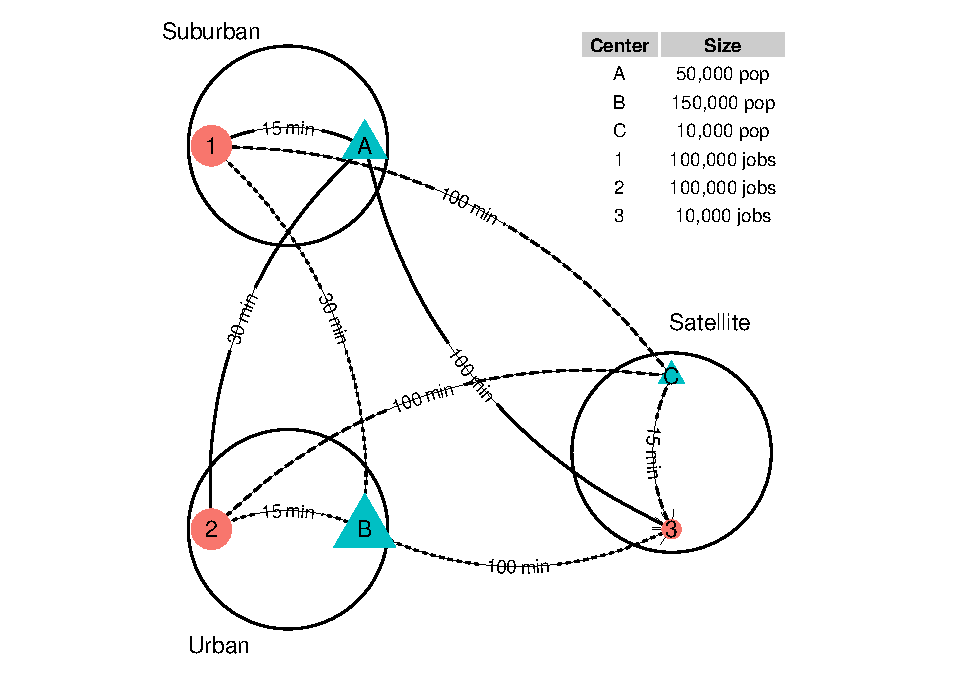
\includegraphics[width=1\linewidth]{Spatial-Availability-Refreshed_files/figure-latex/create-figure-with-toy-example-1} 

}

\caption{\label{fig:plot-toy-example} Shen (1998) synthetic example with locations of employment centers (in orange), population centers (in blue), number of jobs and population, and travel times.}\label{fig:create-figure-with-toy-example}
\end{figure}

 
  \providecommand{\huxb}[2]{\arrayrulecolor[RGB]{#1}\global\arrayrulewidth=#2pt}
  \providecommand{\huxvb}[2]{\color[RGB]{#1}\vrule width #2pt}
  \providecommand{\huxtpad}[1]{\rule{0pt}{#1}}
  \providecommand{\huxbpad}[1]{\rule[-#1]{0pt}{#1}}

\begin{table}[ht]
\begin{centerbox}
\begin{threeparttable}
\captionsetup{justification=centering,singlelinecheck=off}
\caption{Summary description of synthetic example: Hansen-type accessibility and Shen-type accessibility with competition with beta = 0.1}
 \label{tab:synthetic-example}
\setlength{\tabcolsep}{0pt}
\begin{tabularx}{1.2\textwidth}{p{0.12\textwidth} p{0.12\textwidth} p{0.12\textwidth} p{0.12\textwidth} p{0.12\textwidth} p{0.12\textwidth} p{0.12\textwidth} p{0.12\textwidth} p{0.12\textwidth} p{0.12\textwidth}}


\hhline{>{\huxb{190, 190, 190}{1}}|>{\huxb{190, 190, 190}{1}}|>{\huxb{190, 190, 190}{1}}|>{\huxb{190, 190, 190}{1}}|>{\huxb{190, 190, 190}{1}}|>{\huxb{190, 190, 190}{1}}|>{\huxb{190, 190, 190}{1}}|>{\huxb{190, 190, 190}{1}}|>{\huxb{190, 190, 190}{1}}|}
\arrayrulecolor{black}

\multicolumn{1}{!{\huxvb{0, 0, 0}{0}}p{0.12\textwidth}!{\huxvb{190, 190, 190}{1}}}{\hspace{6pt}\parbox[b]{0.12\textwidth-6pt-6pt}{\huxtpad{6pt + 1em}\raggedright \textbf{{\fontsize{7pt}{8.4pt}\selectfont Origin}}\huxbpad{6pt}}} &
\multicolumn{1}{p{0.12\textwidth}!{\huxvb{190, 190, 190}{1}}}{\hspace{6pt}\parbox[b]{0.12\textwidth-6pt-6pt}{\huxtpad{6pt + 1em}\centering \textbf{{\fontsize{7pt}{8.4pt}\selectfont Pop.}}\huxbpad{6pt}}} &
\multicolumn{1}{p{0.12\textwidth}!{\huxvb{190, 190, 190}{1}}}{\hspace{6pt}\parbox[b]{0.12\textwidth-6pt-6pt}{\huxtpad{6pt + 1em}\raggedright \textbf{{\fontsize{7pt}{8.4pt}\selectfont Dest.}}\huxbpad{6pt}}} &
\multicolumn{1}{p{0.12\textwidth}!{\huxvb{190, 190, 190}{1}}}{\hspace{6pt}\parbox[b]{0.12\textwidth-6pt-6pt}{\huxtpad{6pt + 1em}\centering \textbf{{\fontsize{7pt}{8.4pt}\selectfont Jobs}}\huxbpad{6pt}}} &
\multicolumn{1}{p{0.12\textwidth}!{\huxvb{190, 190, 190}{1}}}{\hspace{6pt}\parbox[b]{0.12\textwidth-6pt-6pt}{\huxtpad{6pt + 1em}\centering \textbf{{\fontsize{7pt}{8.4pt}\selectfont TT}}\huxbpad{6pt}}} &
\multicolumn{1}{p{0.12\textwidth}!{\huxvb{190, 190, 190}{1}}}{\hspace{6pt}\parbox[b]{0.12\textwidth-6pt-6pt}{\huxtpad{6pt + 1em}\centering \textbf{{\fontsize{7pt}{8.4pt}\selectfont f(TT)}}\huxbpad{6pt}}} &
\multicolumn{1}{p{0.12\textwidth}!{\huxvb{190, 190, 190}{1}}}{\hspace{6pt}\parbox[b]{0.12\textwidth-6pt-6pt}{\huxtpad{6pt + 1em}\centering \textbf{{\fontsize{7pt}{8.4pt}\selectfont Pop * f(TT)}}\huxbpad{6pt}}} &
\multicolumn{1}{p{0.12\textwidth}!{\huxvb{190, 190, 190}{1}}}{\hspace{6pt}\parbox[b]{0.12\textwidth-6pt-6pt}{\huxtpad{6pt + 1em}\centering \textbf{{\fontsize{7pt}{8.4pt}\selectfont Jobs * f(TT)}}\huxbpad{6pt}}} &
\multicolumn{1}{p{0.12\textwidth}!{\huxvb{190, 190, 190}{1}}}{\hspace{6pt}\parbox[b]{0.12\textwidth-6pt-6pt}{\huxtpad{6pt + 1em}\centering \textbf{{\fontsize{7pt}{8.4pt}\selectfont S\_i}}\huxbpad{6pt}}} &
\multicolumn{1}{p{0.12\textwidth}!{\huxvb{0, 0, 0}{0}}}{\hspace{6pt}\parbox[b]{0.12\textwidth-6pt-6pt}{\huxtpad{6pt + 1em}\centering \textbf{{\fontsize{7pt}{8.4pt}\selectfont a\_i}}\huxbpad{6pt}}} \tabularnewline[-0.5pt]


\hhline{>{\huxb{0, 0, 0}{0.4}}->{\huxb{0, 0, 0}{0.4}}->{\huxb{0, 0, 0}{0.4}}->{\huxb{0, 0, 0}{0.4}}->{\huxb{0, 0, 0}{0.4}}->{\huxb{0, 0, 0}{0.4}}->{\huxb{0, 0, 0}{0.4}}->{\huxb{0, 0, 0}{0.4}}->{\huxb{0, 0, 0}{0.4}}->{\huxb{0, 0, 0}{0.4}}-}
\arrayrulecolor{black}

\multicolumn{1}{!{\huxvb{0, 0, 0}{0}}p{0.12\textwidth}!{\huxvb{190, 190, 190}{1}}}{} &
\multicolumn{1}{p{0.12\textwidth}!{\huxvb{190, 190, 190}{1}}}{} &
\multicolumn{1}{p{0.12\textwidth}!{\huxvb{190, 190, 190}{1}}}{\hspace{6pt}\parbox[b]{0.12\textwidth-6pt-6pt}{\huxtpad{6pt + 1em}\raggedright {\fontsize{7pt}{8.4pt}\selectfont 1}\huxbpad{6pt}}} &
\multicolumn{1}{p{0.12\textwidth}!{\huxvb{190, 190, 190}{1}}}{\hspace{6pt}\parbox[b]{0.12\textwidth-6pt-6pt}{\huxtpad{6pt + 1em}\centering {\fontsize{7pt}{8.4pt}\selectfont 100,000}\huxbpad{6pt}}} &
\multicolumn{1}{p{0.12\textwidth}!{\huxvb{190, 190, 190}{1}}}{\hspace{6pt}\parbox[b]{0.12\textwidth-6pt-6pt}{\huxtpad{6pt + 1em}\centering {\fontsize{7pt}{8.4pt}\selectfont 15}\huxbpad{6pt}}} &
\multicolumn{1}{p{0.12\textwidth}!{\huxvb{190, 190, 190}{1}}}{\hspace{6pt}\parbox[b]{0.12\textwidth-6pt-6pt}{\huxtpad{6pt + 1em}\centering {\fontsize{7pt}{8.4pt}\selectfont 0.223130}\huxbpad{6pt}}} &
\multicolumn{1}{p{0.12\textwidth}!{\huxvb{190, 190, 190}{1}}}{\hspace{6pt}\parbox[b]{0.12\textwidth-6pt-6pt}{\huxtpad{6pt + 1em}\centering {\fontsize{7pt}{8.4pt}\selectfont 11,157}\huxbpad{6pt}}} &
\multicolumn{1}{p{0.12\textwidth}!{\huxvb{190, 190, 190}{1}}}{\hspace{6pt}\parbox[b]{0.12\textwidth-6pt-6pt}{\huxtpad{6pt + 1em}\centering {\fontsize{7pt}{8.4pt}\selectfont 22,313}\huxbpad{6pt}}} &
\multicolumn{1}{p{0.12\textwidth}!{\huxvb{190, 190, 190}{1}}}{} &
\multicolumn{1}{p{0.12\textwidth}!{\huxvb{0, 0, 0}{0}}}{} \tabularnewline[-0.5pt]


\hhline{>{\huxb{190, 190, 190}{1}}|>{\huxb{190, 190, 190}{1}}|>{\huxb{190, 190, 190}{1}}|>{\huxb{190, 190, 190}{1}}|>{\huxb{190, 190, 190}{1}}|>{\huxb{190, 190, 190}{1}}|>{\huxb{190, 190, 190}{1}}|>{\huxb{190, 190, 190}{1}}|>{\huxb{190, 190, 190}{1}}|}
\arrayrulecolor{black}

\multicolumn{1}{!{\huxvb{0, 0, 0}{0}}p{0.12\textwidth}!{\huxvb{190, 190, 190}{1}}}{} &
\multicolumn{1}{p{0.12\textwidth}!{\huxvb{190, 190, 190}{1}}}{} &
\multicolumn{1}{p{0.12\textwidth}!{\huxvb{190, 190, 190}{1}}}{\hspace{6pt}\parbox[b]{0.12\textwidth-6pt-6pt}{\huxtpad{6pt + 1em}\raggedright {\fontsize{7pt}{8.4pt}\selectfont 2}\huxbpad{6pt}}} &
\multicolumn{1}{p{0.12\textwidth}!{\huxvb{190, 190, 190}{1}}}{\hspace{6pt}\parbox[b]{0.12\textwidth-6pt-6pt}{\huxtpad{6pt + 1em}\centering {\fontsize{7pt}{8.4pt}\selectfont 100,000}\huxbpad{6pt}}} &
\multicolumn{1}{p{0.12\textwidth}!{\huxvb{190, 190, 190}{1}}}{\hspace{6pt}\parbox[b]{0.12\textwidth-6pt-6pt}{\huxtpad{6pt + 1em}\centering {\fontsize{7pt}{8.4pt}\selectfont 30}\huxbpad{6pt}}} &
\multicolumn{1}{p{0.12\textwidth}!{\huxvb{190, 190, 190}{1}}}{\hspace{6pt}\parbox[b]{0.12\textwidth-6pt-6pt}{\huxtpad{6pt + 1em}\centering {\fontsize{7pt}{8.4pt}\selectfont 0.049787}\huxbpad{6pt}}} &
\multicolumn{1}{p{0.12\textwidth}!{\huxvb{190, 190, 190}{1}}}{\hspace{6pt}\parbox[b]{0.12\textwidth-6pt-6pt}{\huxtpad{6pt + 1em}\centering {\fontsize{7pt}{8.4pt}\selectfont 2,489}\huxbpad{6pt}}} &
\multicolumn{1}{p{0.12\textwidth}!{\huxvb{190, 190, 190}{1}}}{\hspace{6pt}\parbox[b]{0.12\textwidth-6pt-6pt}{\huxtpad{6pt + 1em}\centering {\fontsize{7pt}{8.4pt}\selectfont 4,979}\huxbpad{6pt}}} &
\multicolumn{1}{p{0.12\textwidth}!{\huxvb{190, 190, 190}{1}}}{} &
\multicolumn{1}{p{0.12\textwidth}!{\huxvb{0, 0, 0}{0}}}{} \tabularnewline[-0.5pt]


\hhline{>{\huxb{190, 190, 190}{1}}|>{\huxb{190, 190, 190}{1}}|>{\huxb{190, 190, 190}{1}}|>{\huxb{190, 190, 190}{1}}|>{\huxb{190, 190, 190}{1}}|>{\huxb{190, 190, 190}{1}}|>{\huxb{190, 190, 190}{1}}|>{\huxb{190, 190, 190}{1}}|>{\huxb{190, 190, 190}{1}}|}
\arrayrulecolor{black}

\multicolumn{1}{!{\huxvb{0, 0, 0}{0}}p{0.12\textwidth}!{\huxvb{190, 190, 190}{1}}}{\multirow[t]{-3}{*}[0ex]{\hspace{6pt}\parbox[b]{0.12\textwidth-6pt-6pt}{\huxtpad{6pt + 1em}\raggedright {\fontsize{7pt}{8.4pt}\selectfont A}\huxbpad{6pt}}}} &
\multicolumn{1}{p{0.12\textwidth}!{\huxvb{190, 190, 190}{1}}}{\multirow[t]{-3}{*}[0ex]{\hspace{6pt}\parbox[b]{0.12\textwidth-6pt-6pt}{\huxtpad{6pt + 1em}\centering {\fontsize{7pt}{8.4pt}\selectfont 50,000}\huxbpad{6pt}}}} &
\multicolumn{1}{p{0.12\textwidth}!{\huxvb{190, 190, 190}{1}}}{\hspace{6pt}\parbox[b]{0.12\textwidth-6pt-6pt}{\huxtpad{6pt + 1em}\raggedright {\fontsize{7pt}{8.4pt}\selectfont 3}\huxbpad{6pt}}} &
\multicolumn{1}{p{0.12\textwidth}!{\huxvb{190, 190, 190}{1}}}{\hspace{6pt}\parbox[b]{0.12\textwidth-6pt-6pt}{\huxtpad{6pt + 1em}\centering {\fontsize{7pt}{8.4pt}\selectfont 10,000}\huxbpad{6pt}}} &
\multicolumn{1}{p{0.12\textwidth}!{\huxvb{190, 190, 190}{1}}}{\hspace{6pt}\parbox[b]{0.12\textwidth-6pt-6pt}{\huxtpad{6pt + 1em}\centering {\fontsize{7pt}{8.4pt}\selectfont 100}\huxbpad{6pt}}} &
\multicolumn{1}{p{0.12\textwidth}!{\huxvb{190, 190, 190}{1}}}{\hspace{6pt}\parbox[b]{0.12\textwidth-6pt-6pt}{\huxtpad{6pt + 1em}\centering {\fontsize{7pt}{8.4pt}\selectfont 0.000045}\huxbpad{6pt}}} &
\multicolumn{1}{p{0.12\textwidth}!{\huxvb{190, 190, 190}{1}}}{\hspace{6pt}\parbox[b]{0.12\textwidth-6pt-6pt}{\huxtpad{6pt + 1em}\centering {\fontsize{7pt}{8.4pt}\selectfont 2.27}\huxbpad{6pt}}} &
\multicolumn{1}{p{0.12\textwidth}!{\huxvb{190, 190, 190}{1}}}{\hspace{6pt}\parbox[b]{0.12\textwidth-6pt-6pt}{\huxtpad{6pt + 1em}\centering {\fontsize{7pt}{8.4pt}\selectfont 0.454}\huxbpad{6pt}}} &
\multicolumn{1}{p{0.12\textwidth}!{\huxvb{190, 190, 190}{1}}}{\multirow[t]{-3}{*}[0ex]{\hspace{6pt}\parbox[b]{0.12\textwidth-6pt-6pt}{\huxtpad{6pt + 1em}\centering {\fontsize{7pt}{8.4pt}\selectfont 27,292}\huxbpad{6pt}}}} &
\multicolumn{1}{p{0.12\textwidth}!{\huxvb{0, 0, 0}{0}}}{\multirow[t]{-3}{*}[0ex]{\hspace{6pt}\parbox[b]{0.12\textwidth-6pt-6pt}{\huxtpad{6pt + 1em}\centering {\fontsize{7pt}{8.4pt}\selectfont 1.34}\huxbpad{6pt}}}} \tabularnewline[-0.5pt]


\hhline{>{\huxb{0, 0, 0}{0.4}}->{\huxb{0, 0, 0}{0.4}}->{\huxb{0, 0, 0}{0.4}}->{\huxb{0, 0, 0}{0.4}}->{\huxb{0, 0, 0}{0.4}}->{\huxb{0, 0, 0}{0.4}}->{\huxb{0, 0, 0}{0.4}}->{\huxb{0, 0, 0}{0.4}}->{\huxb{0, 0, 0}{0.4}}->{\huxb{0, 0, 0}{0.4}}-}
\arrayrulecolor{black}

\multicolumn{1}{!{\huxvb{0, 0, 0}{0}}p{0.12\textwidth}!{\huxvb{190, 190, 190}{1}}}{} &
\multicolumn{1}{p{0.12\textwidth}!{\huxvb{190, 190, 190}{1}}}{} &
\multicolumn{1}{p{0.12\textwidth}!{\huxvb{190, 190, 190}{1}}}{\hspace{6pt}\parbox[b]{0.12\textwidth-6pt-6pt}{\huxtpad{6pt + 1em}\raggedright {\fontsize{7pt}{8.4pt}\selectfont 1}\huxbpad{6pt}}} &
\multicolumn{1}{p{0.12\textwidth}!{\huxvb{190, 190, 190}{1}}}{\hspace{6pt}\parbox[b]{0.12\textwidth-6pt-6pt}{\huxtpad{6pt + 1em}\centering {\fontsize{7pt}{8.4pt}\selectfont 100,000}\huxbpad{6pt}}} &
\multicolumn{1}{p{0.12\textwidth}!{\huxvb{190, 190, 190}{1}}}{\hspace{6pt}\parbox[b]{0.12\textwidth-6pt-6pt}{\huxtpad{6pt + 1em}\centering {\fontsize{7pt}{8.4pt}\selectfont 30}\huxbpad{6pt}}} &
\multicolumn{1}{p{0.12\textwidth}!{\huxvb{190, 190, 190}{1}}}{\hspace{6pt}\parbox[b]{0.12\textwidth-6pt-6pt}{\huxtpad{6pt + 1em}\centering {\fontsize{7pt}{8.4pt}\selectfont 0.049787}\huxbpad{6pt}}} &
\multicolumn{1}{p{0.12\textwidth}!{\huxvb{190, 190, 190}{1}}}{\hspace{6pt}\parbox[b]{0.12\textwidth-6pt-6pt}{\huxtpad{6pt + 1em}\centering {\fontsize{7pt}{8.4pt}\selectfont 7,468}\huxbpad{6pt}}} &
\multicolumn{1}{p{0.12\textwidth}!{\huxvb{190, 190, 190}{1}}}{\hspace{6pt}\parbox[b]{0.12\textwidth-6pt-6pt}{\huxtpad{6pt + 1em}\centering {\fontsize{7pt}{8.4pt}\selectfont 4,979}\huxbpad{6pt}}} &
\multicolumn{1}{p{0.12\textwidth}!{\huxvb{190, 190, 190}{1}}}{} &
\multicolumn{1}{p{0.12\textwidth}!{\huxvb{0, 0, 0}{0}}}{} \tabularnewline[-0.5pt]


\hhline{>{\huxb{190, 190, 190}{1}}|>{\huxb{190, 190, 190}{1}}|>{\huxb{190, 190, 190}{1}}|>{\huxb{190, 190, 190}{1}}|>{\huxb{190, 190, 190}{1}}|>{\huxb{190, 190, 190}{1}}|>{\huxb{190, 190, 190}{1}}|>{\huxb{190, 190, 190}{1}}|>{\huxb{190, 190, 190}{1}}|}
\arrayrulecolor{black}

\multicolumn{1}{!{\huxvb{0, 0, 0}{0}}p{0.12\textwidth}!{\huxvb{190, 190, 190}{1}}}{} &
\multicolumn{1}{p{0.12\textwidth}!{\huxvb{190, 190, 190}{1}}}{} &
\multicolumn{1}{p{0.12\textwidth}!{\huxvb{190, 190, 190}{1}}}{\hspace{6pt}\parbox[b]{0.12\textwidth-6pt-6pt}{\huxtpad{6pt + 1em}\raggedright {\fontsize{7pt}{8.4pt}\selectfont 2}\huxbpad{6pt}}} &
\multicolumn{1}{p{0.12\textwidth}!{\huxvb{190, 190, 190}{1}}}{\hspace{6pt}\parbox[b]{0.12\textwidth-6pt-6pt}{\huxtpad{6pt + 1em}\centering {\fontsize{7pt}{8.4pt}\selectfont 100,000}\huxbpad{6pt}}} &
\multicolumn{1}{p{0.12\textwidth}!{\huxvb{190, 190, 190}{1}}}{\hspace{6pt}\parbox[b]{0.12\textwidth-6pt-6pt}{\huxtpad{6pt + 1em}\centering {\fontsize{7pt}{8.4pt}\selectfont 15}\huxbpad{6pt}}} &
\multicolumn{1}{p{0.12\textwidth}!{\huxvb{190, 190, 190}{1}}}{\hspace{6pt}\parbox[b]{0.12\textwidth-6pt-6pt}{\huxtpad{6pt + 1em}\centering {\fontsize{7pt}{8.4pt}\selectfont 0.223130}\huxbpad{6pt}}} &
\multicolumn{1}{p{0.12\textwidth}!{\huxvb{190, 190, 190}{1}}}{\hspace{6pt}\parbox[b]{0.12\textwidth-6pt-6pt}{\huxtpad{6pt + 1em}\centering {\fontsize{7pt}{8.4pt}\selectfont 33,470}\huxbpad{6pt}}} &
\multicolumn{1}{p{0.12\textwidth}!{\huxvb{190, 190, 190}{1}}}{\hspace{6pt}\parbox[b]{0.12\textwidth-6pt-6pt}{\huxtpad{6pt + 1em}\centering {\fontsize{7pt}{8.4pt}\selectfont 22,313}\huxbpad{6pt}}} &
\multicolumn{1}{p{0.12\textwidth}!{\huxvb{190, 190, 190}{1}}}{} &
\multicolumn{1}{p{0.12\textwidth}!{\huxvb{0, 0, 0}{0}}}{} \tabularnewline[-0.5pt]


\hhline{>{\huxb{190, 190, 190}{1}}|>{\huxb{190, 190, 190}{1}}|>{\huxb{190, 190, 190}{1}}|>{\huxb{190, 190, 190}{1}}|>{\huxb{190, 190, 190}{1}}|>{\huxb{190, 190, 190}{1}}|>{\huxb{190, 190, 190}{1}}|>{\huxb{190, 190, 190}{1}}|>{\huxb{190, 190, 190}{1}}|}
\arrayrulecolor{black}

\multicolumn{1}{!{\huxvb{0, 0, 0}{0}}p{0.12\textwidth}!{\huxvb{190, 190, 190}{1}}}{\multirow[t]{-3}{*}[0ex]{\hspace{6pt}\parbox[b]{0.12\textwidth-6pt-6pt}{\huxtpad{6pt + 1em}\raggedright {\fontsize{7pt}{8.4pt}\selectfont B}\huxbpad{6pt}}}} &
\multicolumn{1}{p{0.12\textwidth}!{\huxvb{190, 190, 190}{1}}}{\multirow[t]{-3}{*}[0ex]{\hspace{6pt}\parbox[b]{0.12\textwidth-6pt-6pt}{\huxtpad{6pt + 1em}\centering {\fontsize{7pt}{8.4pt}\selectfont 150,000}\huxbpad{6pt}}}} &
\multicolumn{1}{p{0.12\textwidth}!{\huxvb{190, 190, 190}{1}}}{\hspace{6pt}\parbox[b]{0.12\textwidth-6pt-6pt}{\huxtpad{6pt + 1em}\raggedright {\fontsize{7pt}{8.4pt}\selectfont 3}\huxbpad{6pt}}} &
\multicolumn{1}{p{0.12\textwidth}!{\huxvb{190, 190, 190}{1}}}{\hspace{6pt}\parbox[b]{0.12\textwidth-6pt-6pt}{\huxtpad{6pt + 1em}\centering {\fontsize{7pt}{8.4pt}\selectfont 10,000}\huxbpad{6pt}}} &
\multicolumn{1}{p{0.12\textwidth}!{\huxvb{190, 190, 190}{1}}}{\hspace{6pt}\parbox[b]{0.12\textwidth-6pt-6pt}{\huxtpad{6pt + 1em}\centering {\fontsize{7pt}{8.4pt}\selectfont 100}\huxbpad{6pt}}} &
\multicolumn{1}{p{0.12\textwidth}!{\huxvb{190, 190, 190}{1}}}{\hspace{6pt}\parbox[b]{0.12\textwidth-6pt-6pt}{\huxtpad{6pt + 1em}\centering {\fontsize{7pt}{8.4pt}\selectfont 0.000045}\huxbpad{6pt}}} &
\multicolumn{1}{p{0.12\textwidth}!{\huxvb{190, 190, 190}{1}}}{\hspace{6pt}\parbox[b]{0.12\textwidth-6pt-6pt}{\huxtpad{6pt + 1em}\centering {\fontsize{7pt}{8.4pt}\selectfont 6.81}\huxbpad{6pt}}} &
\multicolumn{1}{p{0.12\textwidth}!{\huxvb{190, 190, 190}{1}}}{\hspace{6pt}\parbox[b]{0.12\textwidth-6pt-6pt}{\huxtpad{6pt + 1em}\centering {\fontsize{7pt}{8.4pt}\selectfont 0.454}\huxbpad{6pt}}} &
\multicolumn{1}{p{0.12\textwidth}!{\huxvb{190, 190, 190}{1}}}{\multirow[t]{-3}{*}[0ex]{\hspace{6pt}\parbox[b]{0.12\textwidth-6pt-6pt}{\huxtpad{6pt + 1em}\centering {\fontsize{7pt}{8.4pt}\selectfont 27,292}\huxbpad{6pt}}}} &
\multicolumn{1}{p{0.12\textwidth}!{\huxvb{0, 0, 0}{0}}}{\multirow[t]{-3}{*}[0ex]{\hspace{6pt}\parbox[b]{0.12\textwidth-6pt-6pt}{\huxtpad{6pt + 1em}\centering {\fontsize{7pt}{8.4pt}\selectfont 0.888}\huxbpad{6pt}}}} \tabularnewline[-0.5pt]


\hhline{>{\huxb{0, 0, 0}{0.4}}->{\huxb{0, 0, 0}{0.4}}->{\huxb{0, 0, 0}{0.4}}->{\huxb{0, 0, 0}{0.4}}->{\huxb{0, 0, 0}{0.4}}->{\huxb{0, 0, 0}{0.4}}->{\huxb{0, 0, 0}{0.4}}->{\huxb{0, 0, 0}{0.4}}->{\huxb{0, 0, 0}{0.4}}->{\huxb{0, 0, 0}{0.4}}-}
\arrayrulecolor{black}

\multicolumn{1}{!{\huxvb{0, 0, 0}{0}}p{0.12\textwidth}!{\huxvb{190, 190, 190}{1}}}{} &
\multicolumn{1}{p{0.12\textwidth}!{\huxvb{190, 190, 190}{1}}}{} &
\multicolumn{1}{p{0.12\textwidth}!{\huxvb{190, 190, 190}{1}}}{\hspace{6pt}\parbox[b]{0.12\textwidth-6pt-6pt}{\huxtpad{6pt + 1em}\raggedright {\fontsize{7pt}{8.4pt}\selectfont 1}\huxbpad{6pt}}} &
\multicolumn{1}{p{0.12\textwidth}!{\huxvb{190, 190, 190}{1}}}{\hspace{6pt}\parbox[b]{0.12\textwidth-6pt-6pt}{\huxtpad{6pt + 1em}\centering {\fontsize{7pt}{8.4pt}\selectfont 100,000}\huxbpad{6pt}}} &
\multicolumn{1}{p{0.12\textwidth}!{\huxvb{190, 190, 190}{1}}}{\hspace{6pt}\parbox[b]{0.12\textwidth-6pt-6pt}{\huxtpad{6pt + 1em}\centering {\fontsize{7pt}{8.4pt}\selectfont 100}\huxbpad{6pt}}} &
\multicolumn{1}{p{0.12\textwidth}!{\huxvb{190, 190, 190}{1}}}{\hspace{6pt}\parbox[b]{0.12\textwidth-6pt-6pt}{\huxtpad{6pt + 1em}\centering {\fontsize{7pt}{8.4pt}\selectfont 0.000045}\huxbpad{6pt}}} &
\multicolumn{1}{p{0.12\textwidth}!{\huxvb{190, 190, 190}{1}}}{\hspace{6pt}\parbox[b]{0.12\textwidth-6pt-6pt}{\huxtpad{6pt + 1em}\centering {\fontsize{7pt}{8.4pt}\selectfont 0.454}\huxbpad{6pt}}} &
\multicolumn{1}{p{0.12\textwidth}!{\huxvb{190, 190, 190}{1}}}{\hspace{6pt}\parbox[b]{0.12\textwidth-6pt-6pt}{\huxtpad{6pt + 1em}\centering {\fontsize{7pt}{8.4pt}\selectfont 4.54}\huxbpad{6pt}}} &
\multicolumn{1}{p{0.12\textwidth}!{\huxvb{190, 190, 190}{1}}}{} &
\multicolumn{1}{p{0.12\textwidth}!{\huxvb{0, 0, 0}{0}}}{} \tabularnewline[-0.5pt]


\hhline{>{\huxb{190, 190, 190}{1}}|>{\huxb{190, 190, 190}{1}}|>{\huxb{190, 190, 190}{1}}|>{\huxb{190, 190, 190}{1}}|>{\huxb{190, 190, 190}{1}}|>{\huxb{190, 190, 190}{1}}|>{\huxb{190, 190, 190}{1}}|>{\huxb{190, 190, 190}{1}}|>{\huxb{190, 190, 190}{1}}|}
\arrayrulecolor{black}

\multicolumn{1}{!{\huxvb{0, 0, 0}{0}}p{0.12\textwidth}!{\huxvb{190, 190, 190}{1}}}{} &
\multicolumn{1}{p{0.12\textwidth}!{\huxvb{190, 190, 190}{1}}}{} &
\multicolumn{1}{p{0.12\textwidth}!{\huxvb{190, 190, 190}{1}}}{\hspace{6pt}\parbox[b]{0.12\textwidth-6pt-6pt}{\huxtpad{6pt + 1em}\raggedright {\fontsize{7pt}{8.4pt}\selectfont 2}\huxbpad{6pt}}} &
\multicolumn{1}{p{0.12\textwidth}!{\huxvb{190, 190, 190}{1}}}{\hspace{6pt}\parbox[b]{0.12\textwidth-6pt-6pt}{\huxtpad{6pt + 1em}\centering {\fontsize{7pt}{8.4pt}\selectfont 100,000}\huxbpad{6pt}}} &
\multicolumn{1}{p{0.12\textwidth}!{\huxvb{190, 190, 190}{1}}}{\hspace{6pt}\parbox[b]{0.12\textwidth-6pt-6pt}{\huxtpad{6pt + 1em}\centering {\fontsize{7pt}{8.4pt}\selectfont 100}\huxbpad{6pt}}} &
\multicolumn{1}{p{0.12\textwidth}!{\huxvb{190, 190, 190}{1}}}{\hspace{6pt}\parbox[b]{0.12\textwidth-6pt-6pt}{\huxtpad{6pt + 1em}\centering {\fontsize{7pt}{8.4pt}\selectfont 0.000045}\huxbpad{6pt}}} &
\multicolumn{1}{p{0.12\textwidth}!{\huxvb{190, 190, 190}{1}}}{\hspace{6pt}\parbox[b]{0.12\textwidth-6pt-6pt}{\huxtpad{6pt + 1em}\centering {\fontsize{7pt}{8.4pt}\selectfont 0.454}\huxbpad{6pt}}} &
\multicolumn{1}{p{0.12\textwidth}!{\huxvb{190, 190, 190}{1}}}{\hspace{6pt}\parbox[b]{0.12\textwidth-6pt-6pt}{\huxtpad{6pt + 1em}\centering {\fontsize{7pt}{8.4pt}\selectfont 4.54}\huxbpad{6pt}}} &
\multicolumn{1}{p{0.12\textwidth}!{\huxvb{190, 190, 190}{1}}}{} &
\multicolumn{1}{p{0.12\textwidth}!{\huxvb{0, 0, 0}{0}}}{} \tabularnewline[-0.5pt]


\hhline{>{\huxb{190, 190, 190}{1}}|>{\huxb{190, 190, 190}{1}}|>{\huxb{190, 190, 190}{1}}|>{\huxb{190, 190, 190}{1}}|>{\huxb{190, 190, 190}{1}}|>{\huxb{190, 190, 190}{1}}|>{\huxb{190, 190, 190}{1}}|>{\huxb{190, 190, 190}{1}}|>{\huxb{190, 190, 190}{1}}|}
\arrayrulecolor{black}

\multicolumn{1}{!{\huxvb{0, 0, 0}{0}}p{0.12\textwidth}!{\huxvb{190, 190, 190}{1}}}{\multirow[t]{-3}{*}[0ex]{\hspace{6pt}\parbox[b]{0.12\textwidth-6pt-6pt}{\huxtpad{6pt + 1em}\raggedright {\fontsize{7pt}{8.4pt}\selectfont C}\huxbpad{6pt}}}} &
\multicolumn{1}{p{0.12\textwidth}!{\huxvb{190, 190, 190}{1}}}{\multirow[t]{-3}{*}[0ex]{\hspace{6pt}\parbox[b]{0.12\textwidth-6pt-6pt}{\huxtpad{6pt + 1em}\centering {\fontsize{7pt}{8.4pt}\selectfont 10,000}\huxbpad{6pt}}}} &
\multicolumn{1}{p{0.12\textwidth}!{\huxvb{190, 190, 190}{1}}}{\hspace{6pt}\parbox[b]{0.12\textwidth-6pt-6pt}{\huxtpad{6pt + 1em}\raggedright {\fontsize{7pt}{8.4pt}\selectfont 3}\huxbpad{6pt}}} &
\multicolumn{1}{p{0.12\textwidth}!{\huxvb{190, 190, 190}{1}}}{\hspace{6pt}\parbox[b]{0.12\textwidth-6pt-6pt}{\huxtpad{6pt + 1em}\centering {\fontsize{7pt}{8.4pt}\selectfont 10,000}\huxbpad{6pt}}} &
\multicolumn{1}{p{0.12\textwidth}!{\huxvb{190, 190, 190}{1}}}{\hspace{6pt}\parbox[b]{0.12\textwidth-6pt-6pt}{\huxtpad{6pt + 1em}\centering {\fontsize{7pt}{8.4pt}\selectfont 15}\huxbpad{6pt}}} &
\multicolumn{1}{p{0.12\textwidth}!{\huxvb{190, 190, 190}{1}}}{\hspace{6pt}\parbox[b]{0.12\textwidth-6pt-6pt}{\huxtpad{6pt + 1em}\centering {\fontsize{7pt}{8.4pt}\selectfont 0.223130}\huxbpad{6pt}}} &
\multicolumn{1}{p{0.12\textwidth}!{\huxvb{190, 190, 190}{1}}}{\hspace{6pt}\parbox[b]{0.12\textwidth-6pt-6pt}{\huxtpad{6pt + 1em}\centering {\fontsize{7pt}{8.4pt}\selectfont 2,231}\huxbpad{6pt}}} &
\multicolumn{1}{p{0.12\textwidth}!{\huxvb{190, 190, 190}{1}}}{\hspace{6pt}\parbox[b]{0.12\textwidth-6pt-6pt}{\huxtpad{6pt + 1em}\centering {\fontsize{7pt}{8.4pt}\selectfont 2,231}\huxbpad{6pt}}} &
\multicolumn{1}{p{0.12\textwidth}!{\huxvb{190, 190, 190}{1}}}{\multirow[t]{-3}{*}[0ex]{\hspace{6pt}\parbox[b]{0.12\textwidth-6pt-6pt}{\huxtpad{6pt + 1em}\centering {\fontsize{7pt}{8.4pt}\selectfont 2,240}\huxbpad{6pt}}}} &
\multicolumn{1}{p{0.12\textwidth}!{\huxvb{0, 0, 0}{0}}}{\multirow[t]{-3}{*}[0ex]{\hspace{6pt}\parbox[b]{0.12\textwidth-6pt-6pt}{\huxtpad{6pt + 1em}\centering {\fontsize{7pt}{8.4pt}\selectfont 0.996}\huxbpad{6pt}}}} \tabularnewline[-0.5pt]


\hhline{>{\huxb{190, 190, 190}{1}}|>{\huxb{190, 190, 190}{1}}|>{\huxb{190, 190, 190}{1}}|>{\huxb{190, 190, 190}{1}}|>{\huxb{190, 190, 190}{1}}|>{\huxb{190, 190, 190}{1}}|>{\huxb{190, 190, 190}{1}}|>{\huxb{190, 190, 190}{1}}|>{\huxb{190, 190, 190}{1}}|}
\arrayrulecolor{black}
\end{tabularx}
\end{threeparttable}\par\end{centerbox}

\end{table}
 

Table \ref{tab:synthetic-example} contains the information needed to
calculate \(S_i\) and \(a_i\) for this example. We use a negative
exponential impedance function with \(\beta=0.1\) as done in Shen (1998,
see footnote (5)): \[
f(c_{ij}) = \exp(-\beta\cdot c_{ij})
\] In Table \ref{tab:synthetic-example}, we see that population centers
\(A\) and \(B\) have equal Hansen-type accessibility (\(S_A = S_B=\)
27,292 jobs). On the other hand, the isolated satellite town of \(C\)
has low accessibility (\(S_C=\) 2,240 jobs). But center \(B\), despite
its high accessibility, is a large population center. \(C\), in
contrast, is smaller but also relatively isolated and has a balanced
ratio of jobs (10,0000 jobs) to population (10,000 people). It is
difficult from these outputs to determine whether the accessibility at
\(C\) is better or worse than that at \(A\) or \(B\).

The results are easier to interpret when we consider Shen-type
accessibility. The results indicate that \(a_A \approx\) 1.337 jobs per
capita, \(a_B \approx\) 0.888, and \(a_C\approx\) 0.996. The latter
value is sensible given the jobs-population balance of \(C\). Center
\(A\) is relatively close to a large number of jobs (more jobs than the
population of \(A\)). The opposite is true of \(B\). According to Shen
(1998), the sum of the population-weighted accessibility \(a_i\) is
exactly equal to the number of jobs in the region following Shen's
proof: \[
\begin{array}{l}
\sum_{i=1}^N a_{i} P_i= \sum_{j=1}^JO_j\\
50,000\times 1.3366693 \\
+ 150,000 \times 0.8880224 \\
+ 10,000 \times 0.9963171 = 210,000
\end{array}
\]

As mentioned earlier, this property under Shen's definition of \(P_i\)
\emph{``people in location \(i\) seeking opportunities''} , gives the
impression that all sought jobs are allocated to the people located at
each origin \(i\). In other words, Shen defines \(P_i\) to mean
\(P_{ij}^*\) (i.e., the \emph{effective opportunity-seeking population}
which is already adjusted by travel behaviour) while it in fact should
be simply understood as the full population at \(i\) and it is adjusted
by \(a_i\) which already has travel behaviour embedded in its
formulation. As seen in column \textbf{Pop * f(TT)} in Table
\ref{tab:synthetic-example} (i.e., \(P_{ij}^* = P_i\cdot f(c_{ij})\)),
the number of individuals from population center \(A\) that are
\emph{willing to reach} employment centers 1, 2, and 3 are 11,156,
2,489, and 2,27 respectively. Therefore, the total \emph{effective
opportunity-seeking population} in the system (i.e.,
\(P_A^* = \sum_jP_{Aj}^*\)) is 13,647.27 people, which is considerably
lower than the total population of \(A\) (i.e., \(P_A=\) 50,000 people).
Continuing to understand \(P_i\) to equal \(P_{ij}^*\), we would think
that the proof would actually allocate 56,834.59 jobs in the region (as
demonstrated as follows) instead of the nominal number of jobs in the
region which is over three times this number (i.e., 210,000 jobs). \[
\begin{array}{l}
\sum_{i=1}^N a_{i} P_{ij}^* = ???\\
(11,156.51 + 2,489.35 + 2.26)\times 1.3366693 \\
+ (7,468.06 + 33,469.52 + 6.81)\times 0.8880224\\
+ (4.54 + 4.54 + 2,231.20)\times 0.9963171 \approx 56,834.59
\end{array}
\] Furthermore, even when Shen's \(P_i\) is understood plainly as the
total population at \(i\), the meaning of the proof may still be
ambiguous. The proof can still give the impression that all jobs are
allocated to the total population since total population
(\(\sum_{i=1}^N P_i\)) goes into the equation and total jobs
(\(\sum_{j=1}^JO_j\)) in the region is the result. However, this
impression is incomplete since it does not reflect the quantity of
population which is being allocated jobs and the quantity of population
being considered for jobs; these magnitudes are a product of being
weighted down by the impedance function (which reflects travel
behaviour). Why these magnitudes may be hard to disentangle from \(a_i\)
is because it is presented as a rate (i.e., opportunities per capita).

Let's consider a modification to the example in Table
\ref{tab:synthetic-example-2}, to illustrate how the presentation of
\(a_i\) as a rate obscures the magnitude of \emph{effective
opportunity-seeking population} and how that can impact the
interpretation of the result. We modify the example by increasing the
\(\beta\) to 0.5 (compared to the previous value of 0.1; see Figure
\ref{fig:impedance-functions-comparison}). This modification increases
the cost of travel and thus the impedance function, which is an
expression of the population's relative willingness to travel to
opportunities, reflects a population which is relatively less willing to
travel to opportunities further away compared to the previous \(\beta\)
value.

\begin{figure}
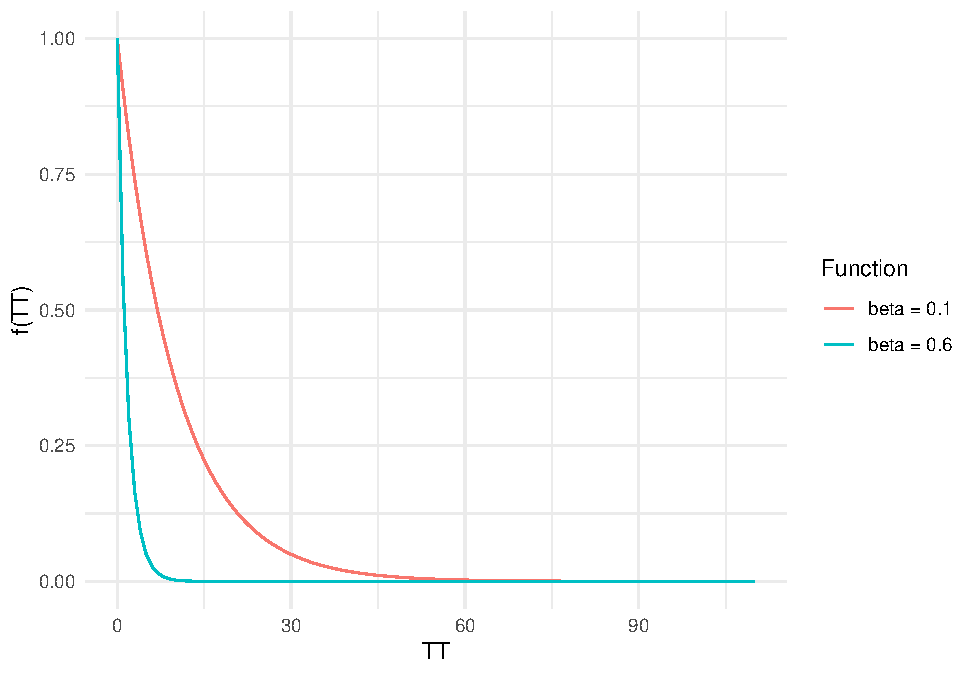
\includegraphics[width=1\linewidth]{Spatial-Availability-Refreshed_files/figure-latex/comparison-impedance-functions-synthetic-example-1} \caption{\label{fig:impedance-functions-comparison}Comparison of two impedance functions in the example.}\label{fig:comparison-impedance-functions-synthetic-example}
\end{figure}

 
  \providecommand{\huxb}[2]{\arrayrulecolor[RGB]{#1}\global\arrayrulewidth=#2pt}
  \providecommand{\huxvb}[2]{\color[RGB]{#1}\vrule width #2pt}
  \providecommand{\huxtpad}[1]{\rule{0pt}{#1}}
  \providecommand{\huxbpad}[1]{\rule[-#1]{0pt}{#1}}

\begin{table}[ht]
\begin{centerbox}
\begin{threeparttable}
\captionsetup{justification=centering,singlelinecheck=off}
\caption{Summary description of synthetic example: Hansen-type accessibility and Shen-type accessibility with competition with beta = 0.5}
 \label{tab:synthetic-example-2}
\setlength{\tabcolsep}{0pt}
\begin{tabularx}{1.3\textwidth}{p{0.13\textwidth} p{0.13\textwidth} p{0.13\textwidth} p{0.13\textwidth} p{0.13\textwidth} p{0.13\textwidth} p{0.13\textwidth} p{0.13\textwidth} p{0.13\textwidth} p{0.13\textwidth}}


\hhline{>{\huxb{190, 190, 190}{1}}|>{\huxb{190, 190, 190}{1}}|>{\huxb{190, 190, 190}{1}}|>{\huxb{190, 190, 190}{1}}|>{\huxb{190, 190, 190}{1}}|>{\huxb{190, 190, 190}{1}}|>{\huxb{190, 190, 190}{1}}|>{\huxb{190, 190, 190}{1}}|>{\huxb{190, 190, 190}{1}}|}
\arrayrulecolor{black}

\multicolumn{1}{!{\huxvb{0, 0, 0}{0}}p{0.13\textwidth}!{\huxvb{190, 190, 190}{1}}}{\hspace{6pt}\parbox[b]{0.13\textwidth-6pt-6pt}{\huxtpad{6pt + 1em}\raggedright \textbf{{\fontsize{7pt}{8.4pt}\selectfont Origin}}\huxbpad{6pt}}} &
\multicolumn{1}{p{0.13\textwidth}!{\huxvb{190, 190, 190}{1}}}{\hspace{6pt}\parbox[b]{0.13\textwidth-6pt-6pt}{\huxtpad{6pt + 1em}\centering \textbf{{\fontsize{7pt}{8.4pt}\selectfont Pop.}}\huxbpad{6pt}}} &
\multicolumn{1}{p{0.13\textwidth}!{\huxvb{190, 190, 190}{1}}}{\hspace{6pt}\parbox[b]{0.13\textwidth-6pt-6pt}{\huxtpad{6pt + 1em}\raggedright \textbf{{\fontsize{7pt}{8.4pt}\selectfont Dest.}}\huxbpad{6pt}}} &
\multicolumn{1}{p{0.13\textwidth}!{\huxvb{190, 190, 190}{1}}}{\hspace{6pt}\parbox[b]{0.13\textwidth-6pt-6pt}{\huxtpad{6pt + 1em}\centering \textbf{{\fontsize{7pt}{8.4pt}\selectfont Jobs}}\huxbpad{6pt}}} &
\multicolumn{1}{p{0.13\textwidth}!{\huxvb{190, 190, 190}{1}}}{\hspace{6pt}\parbox[b]{0.13\textwidth-6pt-6pt}{\huxtpad{6pt + 1em}\centering \textbf{{\fontsize{7pt}{8.4pt}\selectfont TT}}\huxbpad{6pt}}} &
\multicolumn{1}{p{0.13\textwidth}!{\huxvb{190, 190, 190}{1}}}{\hspace{6pt}\parbox[b]{0.13\textwidth-6pt-6pt}{\huxtpad{6pt + 1em}\centering \textbf{{\fontsize{7pt}{8.4pt}\selectfont f(TT)}}\huxbpad{6pt}}} &
\multicolumn{1}{p{0.13\textwidth}!{\huxvb{190, 190, 190}{1}}}{\hspace{6pt}\parbox[b]{0.13\textwidth-6pt-6pt}{\huxtpad{6pt + 1em}\centering \textbf{{\fontsize{7pt}{8.4pt}\selectfont Pop * f(TT)}}\huxbpad{6pt}}} &
\multicolumn{1}{p{0.13\textwidth}!{\huxvb{190, 190, 190}{1}}}{\hspace{6pt}\parbox[b]{0.13\textwidth-6pt-6pt}{\huxtpad{6pt + 1em}\centering \textbf{{\fontsize{7pt}{8.4pt}\selectfont Jobs * f(TT)}}\huxbpad{6pt}}} &
\multicolumn{1}{p{0.13\textwidth}!{\huxvb{190, 190, 190}{1}}}{\hspace{6pt}\parbox[b]{0.13\textwidth-6pt-6pt}{\huxtpad{6pt + 1em}\centering \textbf{{\fontsize{7pt}{8.4pt}\selectfont S\_i}}\huxbpad{6pt}}} &
\multicolumn{1}{p{0.13\textwidth}!{\huxvb{0, 0, 0}{0}}}{\hspace{6pt}\parbox[b]{0.13\textwidth-6pt-6pt}{\huxtpad{6pt + 1em}\centering \textbf{{\fontsize{7pt}{8.4pt}\selectfont a\_i}}\huxbpad{6pt}}} \tabularnewline[-0.5pt]


\hhline{>{\huxb{0, 0, 0}{0.4}}->{\huxb{0, 0, 0}{0.4}}->{\huxb{0, 0, 0}{0.4}}->{\huxb{0, 0, 0}{0.4}}->{\huxb{0, 0, 0}{0.4}}->{\huxb{0, 0, 0}{0.4}}->{\huxb{0, 0, 0}{0.4}}->{\huxb{0, 0, 0}{0.4}}->{\huxb{0, 0, 0}{0.4}}->{\huxb{0, 0, 0}{0.4}}-}
\arrayrulecolor{black}

\multicolumn{1}{!{\huxvb{0, 0, 0}{0}}p{0.13\textwidth}!{\huxvb{190, 190, 190}{1}}}{} &
\multicolumn{1}{p{0.13\textwidth}!{\huxvb{190, 190, 190}{1}}}{} &
\multicolumn{1}{p{0.13\textwidth}!{\huxvb{190, 190, 190}{1}}}{\hspace{6pt}\parbox[b]{0.13\textwidth-6pt-6pt}{\huxtpad{6pt + 1em}\raggedright {\fontsize{7pt}{8.4pt}\selectfont 1}\huxbpad{6pt}}} &
\multicolumn{1}{p{0.13\textwidth}!{\huxvb{190, 190, 190}{1}}}{\hspace{6pt}\parbox[b]{0.13\textwidth-6pt-6pt}{\huxtpad{6pt + 1em}\centering {\fontsize{7pt}{8.4pt}\selectfont 100,000}\huxbpad{6pt}}} &
\multicolumn{1}{p{0.13\textwidth}!{\huxvb{190, 190, 190}{1}}}{\hspace{6pt}\parbox[b]{0.13\textwidth-6pt-6pt}{\huxtpad{6pt + 1em}\centering {\fontsize{7pt}{8.4pt}\selectfont 15}\huxbpad{6pt}}} &
\multicolumn{1}{p{0.13\textwidth}!{\huxvb{190, 190, 190}{1}}}{\hspace{6pt}\parbox[b]{0.13\textwidth-6pt-6pt}{\huxtpad{6pt + 1em}\centering {\fontsize{7pt}{8.4pt}\selectfont $<$ 0.001}\huxbpad{6pt}}} &
\multicolumn{1}{p{0.13\textwidth}!{\huxvb{190, 190, 190}{1}}}{\hspace{6pt}\parbox[b]{0.13\textwidth-6pt-6pt}{\huxtpad{6pt + 1em}\centering {\fontsize{7pt}{8.4pt}\selectfont 0.015}\huxbpad{6pt}}} &
\multicolumn{1}{p{0.13\textwidth}!{\huxvb{190, 190, 190}{1}}}{\hspace{6pt}\parbox[b]{0.13\textwidth-6pt-6pt}{\huxtpad{6pt + 1em}\centering {\fontsize{7pt}{8.4pt}\selectfont 0.031}\huxbpad{6pt}}} &
\multicolumn{1}{p{0.13\textwidth}!{\huxvb{190, 190, 190}{1}}}{} &
\multicolumn{1}{p{0.13\textwidth}!{\huxvb{0, 0, 0}{0}}}{} \tabularnewline[-0.5pt]


\hhline{>{\huxb{190, 190, 190}{1}}|>{\huxb{190, 190, 190}{1}}|>{\huxb{190, 190, 190}{1}}|>{\huxb{190, 190, 190}{1}}|>{\huxb{190, 190, 190}{1}}|>{\huxb{190, 190, 190}{1}}|>{\huxb{190, 190, 190}{1}}|>{\huxb{190, 190, 190}{1}}|>{\huxb{190, 190, 190}{1}}|}
\arrayrulecolor{black}

\multicolumn{1}{!{\huxvb{0, 0, 0}{0}}p{0.13\textwidth}!{\huxvb{190, 190, 190}{1}}}{} &
\multicolumn{1}{p{0.13\textwidth}!{\huxvb{190, 190, 190}{1}}}{} &
\multicolumn{1}{p{0.13\textwidth}!{\huxvb{190, 190, 190}{1}}}{\hspace{6pt}\parbox[b]{0.13\textwidth-6pt-6pt}{\huxtpad{6pt + 1em}\raggedright {\fontsize{7pt}{8.4pt}\selectfont 2}\huxbpad{6pt}}} &
\multicolumn{1}{p{0.13\textwidth}!{\huxvb{190, 190, 190}{1}}}{\hspace{6pt}\parbox[b]{0.13\textwidth-6pt-6pt}{\huxtpad{6pt + 1em}\centering {\fontsize{7pt}{8.4pt}\selectfont 100,000}\huxbpad{6pt}}} &
\multicolumn{1}{p{0.13\textwidth}!{\huxvb{190, 190, 190}{1}}}{\hspace{6pt}\parbox[b]{0.13\textwidth-6pt-6pt}{\huxtpad{6pt + 1em}\centering {\fontsize{7pt}{8.4pt}\selectfont 30}\huxbpad{6pt}}} &
\multicolumn{1}{p{0.13\textwidth}!{\huxvb{190, 190, 190}{1}}}{\hspace{6pt}\parbox[b]{0.13\textwidth-6pt-6pt}{\huxtpad{6pt + 1em}\centering {\fontsize{7pt}{8.4pt}\selectfont $<$ 0.001}\huxbpad{6pt}}} &
\multicolumn{1}{p{0.13\textwidth}!{\huxvb{190, 190, 190}{1}}}{\hspace{6pt}\parbox[b]{0.13\textwidth-6pt-6pt}{\huxtpad{6pt + 1em}\centering {\fontsize{7pt}{8.4pt}\selectfont $<$ 0.001}\huxbpad{6pt}}} &
\multicolumn{1}{p{0.13\textwidth}!{\huxvb{190, 190, 190}{1}}}{\hspace{6pt}\parbox[b]{0.13\textwidth-6pt-6pt}{\huxtpad{6pt + 1em}\centering {\fontsize{7pt}{8.4pt}\selectfont $<$ 0.001}\huxbpad{6pt}}} &
\multicolumn{1}{p{0.13\textwidth}!{\huxvb{190, 190, 190}{1}}}{} &
\multicolumn{1}{p{0.13\textwidth}!{\huxvb{0, 0, 0}{0}}}{} \tabularnewline[-0.5pt]


\hhline{>{\huxb{190, 190, 190}{1}}|>{\huxb{190, 190, 190}{1}}|>{\huxb{190, 190, 190}{1}}|>{\huxb{190, 190, 190}{1}}|>{\huxb{190, 190, 190}{1}}|>{\huxb{190, 190, 190}{1}}|>{\huxb{190, 190, 190}{1}}|>{\huxb{190, 190, 190}{1}}|>{\huxb{190, 190, 190}{1}}|}
\arrayrulecolor{black}

\multicolumn{1}{!{\huxvb{0, 0, 0}{0}}p{0.13\textwidth}!{\huxvb{190, 190, 190}{1}}}{\multirow[t]{-3}{*}[0ex]{\hspace{6pt}\parbox[b]{0.13\textwidth-6pt-6pt}{\huxtpad{6pt + 1em}\raggedright {\fontsize{7pt}{8.4pt}\selectfont A}\huxbpad{6pt}}}} &
\multicolumn{1}{p{0.13\textwidth}!{\huxvb{190, 190, 190}{1}}}{\multirow[t]{-3}{*}[0ex]{\hspace{6pt}\parbox[b]{0.13\textwidth-6pt-6pt}{\huxtpad{6pt + 1em}\centering {\fontsize{7pt}{8.4pt}\selectfont 50,000}\huxbpad{6pt}}}} &
\multicolumn{1}{p{0.13\textwidth}!{\huxvb{190, 190, 190}{1}}}{\hspace{6pt}\parbox[b]{0.13\textwidth-6pt-6pt}{\huxtpad{6pt + 1em}\raggedright {\fontsize{7pt}{8.4pt}\selectfont 3}\huxbpad{6pt}}} &
\multicolumn{1}{p{0.13\textwidth}!{\huxvb{190, 190, 190}{1}}}{\hspace{6pt}\parbox[b]{0.13\textwidth-6pt-6pt}{\huxtpad{6pt + 1em}\centering {\fontsize{7pt}{8.4pt}\selectfont 10,000}\huxbpad{6pt}}} &
\multicolumn{1}{p{0.13\textwidth}!{\huxvb{190, 190, 190}{1}}}{\hspace{6pt}\parbox[b]{0.13\textwidth-6pt-6pt}{\huxtpad{6pt + 1em}\centering {\fontsize{7pt}{8.4pt}\selectfont 100}\huxbpad{6pt}}} &
\multicolumn{1}{p{0.13\textwidth}!{\huxvb{190, 190, 190}{1}}}{\hspace{6pt}\parbox[b]{0.13\textwidth-6pt-6pt}{\huxtpad{6pt + 1em}\centering {\fontsize{7pt}{8.4pt}\selectfont $<$ 0.001}\huxbpad{6pt}}} &
\multicolumn{1}{p{0.13\textwidth}!{\huxvb{190, 190, 190}{1}}}{\hspace{6pt}\parbox[b]{0.13\textwidth-6pt-6pt}{\huxtpad{6pt + 1em}\centering {\fontsize{7pt}{8.4pt}\selectfont $<$ 0.001}\huxbpad{6pt}}} &
\multicolumn{1}{p{0.13\textwidth}!{\huxvb{190, 190, 190}{1}}}{\hspace{6pt}\parbox[b]{0.13\textwidth-6pt-6pt}{\huxtpad{6pt + 1em}\centering {\fontsize{7pt}{8.4pt}\selectfont $<$ 0.001}\huxbpad{6pt}}} &
\multicolumn{1}{p{0.13\textwidth}!{\huxvb{190, 190, 190}{1}}}{\multirow[t]{-3}{*}[0ex]{\hspace{6pt}\parbox[b]{0.13\textwidth-6pt-6pt}{\huxtpad{6pt + 1em}\centering {\fontsize{7pt}{8.4pt}\selectfont 0.0306}\huxbpad{6pt}}}} &
\multicolumn{1}{p{0.13\textwidth}!{\huxvb{0, 0, 0}{0}}}{\multirow[t]{-3}{*}[0ex]{\hspace{6pt}\parbox[b]{0.13\textwidth-6pt-6pt}{\huxtpad{6pt + 1em}\centering {\fontsize{7pt}{8.4pt}\selectfont 2}\huxbpad{6pt}}}} \tabularnewline[-0.5pt]


\hhline{>{\huxb{0, 0, 0}{0.4}}->{\huxb{0, 0, 0}{0.4}}->{\huxb{0, 0, 0}{0.4}}->{\huxb{0, 0, 0}{0.4}}->{\huxb{0, 0, 0}{0.4}}->{\huxb{0, 0, 0}{0.4}}->{\huxb{0, 0, 0}{0.4}}->{\huxb{0, 0, 0}{0.4}}->{\huxb{0, 0, 0}{0.4}}->{\huxb{0, 0, 0}{0.4}}-}
\arrayrulecolor{black}

\multicolumn{1}{!{\huxvb{0, 0, 0}{0}}p{0.13\textwidth}!{\huxvb{190, 190, 190}{1}}}{} &
\multicolumn{1}{p{0.13\textwidth}!{\huxvb{190, 190, 190}{1}}}{} &
\multicolumn{1}{p{0.13\textwidth}!{\huxvb{190, 190, 190}{1}}}{\hspace{6pt}\parbox[b]{0.13\textwidth-6pt-6pt}{\huxtpad{6pt + 1em}\raggedright {\fontsize{7pt}{8.4pt}\selectfont 1}\huxbpad{6pt}}} &
\multicolumn{1}{p{0.13\textwidth}!{\huxvb{190, 190, 190}{1}}}{\hspace{6pt}\parbox[b]{0.13\textwidth-6pt-6pt}{\huxtpad{6pt + 1em}\centering {\fontsize{7pt}{8.4pt}\selectfont 100,000}\huxbpad{6pt}}} &
\multicolumn{1}{p{0.13\textwidth}!{\huxvb{190, 190, 190}{1}}}{\hspace{6pt}\parbox[b]{0.13\textwidth-6pt-6pt}{\huxtpad{6pt + 1em}\centering {\fontsize{7pt}{8.4pt}\selectfont 30}\huxbpad{6pt}}} &
\multicolumn{1}{p{0.13\textwidth}!{\huxvb{190, 190, 190}{1}}}{\hspace{6pt}\parbox[b]{0.13\textwidth-6pt-6pt}{\huxtpad{6pt + 1em}\centering {\fontsize{7pt}{8.4pt}\selectfont $<$ 0.001}\huxbpad{6pt}}} &
\multicolumn{1}{p{0.13\textwidth}!{\huxvb{190, 190, 190}{1}}}{\hspace{6pt}\parbox[b]{0.13\textwidth-6pt-6pt}{\huxtpad{6pt + 1em}\centering {\fontsize{7pt}{8.4pt}\selectfont $<$ 0.001}\huxbpad{6pt}}} &
\multicolumn{1}{p{0.13\textwidth}!{\huxvb{190, 190, 190}{1}}}{\hspace{6pt}\parbox[b]{0.13\textwidth-6pt-6pt}{\huxtpad{6pt + 1em}\centering {\fontsize{7pt}{8.4pt}\selectfont $<$ 0.001}\huxbpad{6pt}}} &
\multicolumn{1}{p{0.13\textwidth}!{\huxvb{190, 190, 190}{1}}}{} &
\multicolumn{1}{p{0.13\textwidth}!{\huxvb{0, 0, 0}{0}}}{} \tabularnewline[-0.5pt]


\hhline{>{\huxb{190, 190, 190}{1}}|>{\huxb{190, 190, 190}{1}}|>{\huxb{190, 190, 190}{1}}|>{\huxb{190, 190, 190}{1}}|>{\huxb{190, 190, 190}{1}}|>{\huxb{190, 190, 190}{1}}|>{\huxb{190, 190, 190}{1}}|>{\huxb{190, 190, 190}{1}}|>{\huxb{190, 190, 190}{1}}|}
\arrayrulecolor{black}

\multicolumn{1}{!{\huxvb{0, 0, 0}{0}}p{0.13\textwidth}!{\huxvb{190, 190, 190}{1}}}{} &
\multicolumn{1}{p{0.13\textwidth}!{\huxvb{190, 190, 190}{1}}}{} &
\multicolumn{1}{p{0.13\textwidth}!{\huxvb{190, 190, 190}{1}}}{\hspace{6pt}\parbox[b]{0.13\textwidth-6pt-6pt}{\huxtpad{6pt + 1em}\raggedright {\fontsize{7pt}{8.4pt}\selectfont 2}\huxbpad{6pt}}} &
\multicolumn{1}{p{0.13\textwidth}!{\huxvb{190, 190, 190}{1}}}{\hspace{6pt}\parbox[b]{0.13\textwidth-6pt-6pt}{\huxtpad{6pt + 1em}\centering {\fontsize{7pt}{8.4pt}\selectfont 100,000}\huxbpad{6pt}}} &
\multicolumn{1}{p{0.13\textwidth}!{\huxvb{190, 190, 190}{1}}}{\hspace{6pt}\parbox[b]{0.13\textwidth-6pt-6pt}{\huxtpad{6pt + 1em}\centering {\fontsize{7pt}{8.4pt}\selectfont 15}\huxbpad{6pt}}} &
\multicolumn{1}{p{0.13\textwidth}!{\huxvb{190, 190, 190}{1}}}{\hspace{6pt}\parbox[b]{0.13\textwidth-6pt-6pt}{\huxtpad{6pt + 1em}\centering {\fontsize{7pt}{8.4pt}\selectfont $<$ 0.001}\huxbpad{6pt}}} &
\multicolumn{1}{p{0.13\textwidth}!{\huxvb{190, 190, 190}{1}}}{\hspace{6pt}\parbox[b]{0.13\textwidth-6pt-6pt}{\huxtpad{6pt + 1em}\centering {\fontsize{7pt}{8.4pt}\selectfont 0.046}\huxbpad{6pt}}} &
\multicolumn{1}{p{0.13\textwidth}!{\huxvb{190, 190, 190}{1}}}{\hspace{6pt}\parbox[b]{0.13\textwidth-6pt-6pt}{\huxtpad{6pt + 1em}\centering {\fontsize{7pt}{8.4pt}\selectfont 0.031}\huxbpad{6pt}}} &
\multicolumn{1}{p{0.13\textwidth}!{\huxvb{190, 190, 190}{1}}}{} &
\multicolumn{1}{p{0.13\textwidth}!{\huxvb{0, 0, 0}{0}}}{} \tabularnewline[-0.5pt]


\hhline{>{\huxb{190, 190, 190}{1}}|>{\huxb{190, 190, 190}{1}}|>{\huxb{190, 190, 190}{1}}|>{\huxb{190, 190, 190}{1}}|>{\huxb{190, 190, 190}{1}}|>{\huxb{190, 190, 190}{1}}|>{\huxb{190, 190, 190}{1}}|>{\huxb{190, 190, 190}{1}}|>{\huxb{190, 190, 190}{1}}|}
\arrayrulecolor{black}

\multicolumn{1}{!{\huxvb{0, 0, 0}{0}}p{0.13\textwidth}!{\huxvb{190, 190, 190}{1}}}{\multirow[t]{-3}{*}[0ex]{\hspace{6pt}\parbox[b]{0.13\textwidth-6pt-6pt}{\huxtpad{6pt + 1em}\raggedright {\fontsize{7pt}{8.4pt}\selectfont B}\huxbpad{6pt}}}} &
\multicolumn{1}{p{0.13\textwidth}!{\huxvb{190, 190, 190}{1}}}{\multirow[t]{-3}{*}[0ex]{\hspace{6pt}\parbox[b]{0.13\textwidth-6pt-6pt}{\huxtpad{6pt + 1em}\centering {\fontsize{7pt}{8.4pt}\selectfont 150,000}\huxbpad{6pt}}}} &
\multicolumn{1}{p{0.13\textwidth}!{\huxvb{190, 190, 190}{1}}}{\hspace{6pt}\parbox[b]{0.13\textwidth-6pt-6pt}{\huxtpad{6pt + 1em}\raggedright {\fontsize{7pt}{8.4pt}\selectfont 3}\huxbpad{6pt}}} &
\multicolumn{1}{p{0.13\textwidth}!{\huxvb{190, 190, 190}{1}}}{\hspace{6pt}\parbox[b]{0.13\textwidth-6pt-6pt}{\huxtpad{6pt + 1em}\centering {\fontsize{7pt}{8.4pt}\selectfont 10,000}\huxbpad{6pt}}} &
\multicolumn{1}{p{0.13\textwidth}!{\huxvb{190, 190, 190}{1}}}{\hspace{6pt}\parbox[b]{0.13\textwidth-6pt-6pt}{\huxtpad{6pt + 1em}\centering {\fontsize{7pt}{8.4pt}\selectfont 100}\huxbpad{6pt}}} &
\multicolumn{1}{p{0.13\textwidth}!{\huxvb{190, 190, 190}{1}}}{\hspace{6pt}\parbox[b]{0.13\textwidth-6pt-6pt}{\huxtpad{6pt + 1em}\centering {\fontsize{7pt}{8.4pt}\selectfont $<$ 0.001}\huxbpad{6pt}}} &
\multicolumn{1}{p{0.13\textwidth}!{\huxvb{190, 190, 190}{1}}}{\hspace{6pt}\parbox[b]{0.13\textwidth-6pt-6pt}{\huxtpad{6pt + 1em}\centering {\fontsize{7pt}{8.4pt}\selectfont $<$ 0.001}\huxbpad{6pt}}} &
\multicolumn{1}{p{0.13\textwidth}!{\huxvb{190, 190, 190}{1}}}{\hspace{6pt}\parbox[b]{0.13\textwidth-6pt-6pt}{\huxtpad{6pt + 1em}\centering {\fontsize{7pt}{8.4pt}\selectfont $<$ 0.001}\huxbpad{6pt}}} &
\multicolumn{1}{p{0.13\textwidth}!{\huxvb{190, 190, 190}{1}}}{\multirow[t]{-3}{*}[0ex]{\hspace{6pt}\parbox[b]{0.13\textwidth-6pt-6pt}{\huxtpad{6pt + 1em}\centering {\fontsize{7pt}{8.4pt}\selectfont 0.0306}\huxbpad{6pt}}}} &
\multicolumn{1}{p{0.13\textwidth}!{\huxvb{0, 0, 0}{0}}}{\multirow[t]{-3}{*}[0ex]{\hspace{6pt}\parbox[b]{0.13\textwidth-6pt-6pt}{\huxtpad{6pt + 1em}\centering {\fontsize{7pt}{8.4pt}\selectfont 0.667}\huxbpad{6pt}}}} \tabularnewline[-0.5pt]


\hhline{>{\huxb{0, 0, 0}{0.4}}->{\huxb{0, 0, 0}{0.4}}->{\huxb{0, 0, 0}{0.4}}->{\huxb{0, 0, 0}{0.4}}->{\huxb{0, 0, 0}{0.4}}->{\huxb{0, 0, 0}{0.4}}->{\huxb{0, 0, 0}{0.4}}->{\huxb{0, 0, 0}{0.4}}->{\huxb{0, 0, 0}{0.4}}->{\huxb{0, 0, 0}{0.4}}-}
\arrayrulecolor{black}

\multicolumn{1}{!{\huxvb{0, 0, 0}{0}}p{0.13\textwidth}!{\huxvb{190, 190, 190}{1}}}{} &
\multicolumn{1}{p{0.13\textwidth}!{\huxvb{190, 190, 190}{1}}}{} &
\multicolumn{1}{p{0.13\textwidth}!{\huxvb{190, 190, 190}{1}}}{\hspace{6pt}\parbox[b]{0.13\textwidth-6pt-6pt}{\huxtpad{6pt + 1em}\raggedright {\fontsize{7pt}{8.4pt}\selectfont 1}\huxbpad{6pt}}} &
\multicolumn{1}{p{0.13\textwidth}!{\huxvb{190, 190, 190}{1}}}{\hspace{6pt}\parbox[b]{0.13\textwidth-6pt-6pt}{\huxtpad{6pt + 1em}\centering {\fontsize{7pt}{8.4pt}\selectfont 100,000}\huxbpad{6pt}}} &
\multicolumn{1}{p{0.13\textwidth}!{\huxvb{190, 190, 190}{1}}}{\hspace{6pt}\parbox[b]{0.13\textwidth-6pt-6pt}{\huxtpad{6pt + 1em}\centering {\fontsize{7pt}{8.4pt}\selectfont 100}\huxbpad{6pt}}} &
\multicolumn{1}{p{0.13\textwidth}!{\huxvb{190, 190, 190}{1}}}{\hspace{6pt}\parbox[b]{0.13\textwidth-6pt-6pt}{\huxtpad{6pt + 1em}\centering {\fontsize{7pt}{8.4pt}\selectfont $<$ 0.001}\huxbpad{6pt}}} &
\multicolumn{1}{p{0.13\textwidth}!{\huxvb{190, 190, 190}{1}}}{\hspace{6pt}\parbox[b]{0.13\textwidth-6pt-6pt}{\huxtpad{6pt + 1em}\centering {\fontsize{7pt}{8.4pt}\selectfont $<$ 0.001}\huxbpad{6pt}}} &
\multicolumn{1}{p{0.13\textwidth}!{\huxvb{190, 190, 190}{1}}}{\hspace{6pt}\parbox[b]{0.13\textwidth-6pt-6pt}{\huxtpad{6pt + 1em}\centering {\fontsize{7pt}{8.4pt}\selectfont $<$ 0.001}\huxbpad{6pt}}} &
\multicolumn{1}{p{0.13\textwidth}!{\huxvb{190, 190, 190}{1}}}{} &
\multicolumn{1}{p{0.13\textwidth}!{\huxvb{0, 0, 0}{0}}}{} \tabularnewline[-0.5pt]


\hhline{>{\huxb{190, 190, 190}{1}}|>{\huxb{190, 190, 190}{1}}|>{\huxb{190, 190, 190}{1}}|>{\huxb{190, 190, 190}{1}}|>{\huxb{190, 190, 190}{1}}|>{\huxb{190, 190, 190}{1}}|>{\huxb{190, 190, 190}{1}}|>{\huxb{190, 190, 190}{1}}|>{\huxb{190, 190, 190}{1}}|}
\arrayrulecolor{black}

\multicolumn{1}{!{\huxvb{0, 0, 0}{0}}p{0.13\textwidth}!{\huxvb{190, 190, 190}{1}}}{} &
\multicolumn{1}{p{0.13\textwidth}!{\huxvb{190, 190, 190}{1}}}{} &
\multicolumn{1}{p{0.13\textwidth}!{\huxvb{190, 190, 190}{1}}}{\hspace{6pt}\parbox[b]{0.13\textwidth-6pt-6pt}{\huxtpad{6pt + 1em}\raggedright {\fontsize{7pt}{8.4pt}\selectfont 2}\huxbpad{6pt}}} &
\multicolumn{1}{p{0.13\textwidth}!{\huxvb{190, 190, 190}{1}}}{\hspace{6pt}\parbox[b]{0.13\textwidth-6pt-6pt}{\huxtpad{6pt + 1em}\centering {\fontsize{7pt}{8.4pt}\selectfont 100,000}\huxbpad{6pt}}} &
\multicolumn{1}{p{0.13\textwidth}!{\huxvb{190, 190, 190}{1}}}{\hspace{6pt}\parbox[b]{0.13\textwidth-6pt-6pt}{\huxtpad{6pt + 1em}\centering {\fontsize{7pt}{8.4pt}\selectfont 100}\huxbpad{6pt}}} &
\multicolumn{1}{p{0.13\textwidth}!{\huxvb{190, 190, 190}{1}}}{\hspace{6pt}\parbox[b]{0.13\textwidth-6pt-6pt}{\huxtpad{6pt + 1em}\centering {\fontsize{7pt}{8.4pt}\selectfont $<$ 0.001}\huxbpad{6pt}}} &
\multicolumn{1}{p{0.13\textwidth}!{\huxvb{190, 190, 190}{1}}}{\hspace{6pt}\parbox[b]{0.13\textwidth-6pt-6pt}{\huxtpad{6pt + 1em}\centering {\fontsize{7pt}{8.4pt}\selectfont $<$ 0.001}\huxbpad{6pt}}} &
\multicolumn{1}{p{0.13\textwidth}!{\huxvb{190, 190, 190}{1}}}{\hspace{6pt}\parbox[b]{0.13\textwidth-6pt-6pt}{\huxtpad{6pt + 1em}\centering {\fontsize{7pt}{8.4pt}\selectfont $<$ 0.001}\huxbpad{6pt}}} &
\multicolumn{1}{p{0.13\textwidth}!{\huxvb{190, 190, 190}{1}}}{} &
\multicolumn{1}{p{0.13\textwidth}!{\huxvb{0, 0, 0}{0}}}{} \tabularnewline[-0.5pt]


\hhline{>{\huxb{190, 190, 190}{1}}|>{\huxb{190, 190, 190}{1}}|>{\huxb{190, 190, 190}{1}}|>{\huxb{190, 190, 190}{1}}|>{\huxb{190, 190, 190}{1}}|>{\huxb{190, 190, 190}{1}}|>{\huxb{190, 190, 190}{1}}|>{\huxb{190, 190, 190}{1}}|>{\huxb{190, 190, 190}{1}}|}
\arrayrulecolor{black}

\multicolumn{1}{!{\huxvb{0, 0, 0}{0}}p{0.13\textwidth}!{\huxvb{190, 190, 190}{1}}}{\multirow[t]{-3}{*}[0ex]{\hspace{6pt}\parbox[b]{0.13\textwidth-6pt-6pt}{\huxtpad{6pt + 1em}\raggedright {\fontsize{7pt}{8.4pt}\selectfont C}\huxbpad{6pt}}}} &
\multicolumn{1}{p{0.13\textwidth}!{\huxvb{190, 190, 190}{1}}}{\multirow[t]{-3}{*}[0ex]{\hspace{6pt}\parbox[b]{0.13\textwidth-6pt-6pt}{\huxtpad{6pt + 1em}\centering {\fontsize{7pt}{8.4pt}\selectfont 10,000}\huxbpad{6pt}}}} &
\multicolumn{1}{p{0.13\textwidth}!{\huxvb{190, 190, 190}{1}}}{\hspace{6pt}\parbox[b]{0.13\textwidth-6pt-6pt}{\huxtpad{6pt + 1em}\raggedright {\fontsize{7pt}{8.4pt}\selectfont 3}\huxbpad{6pt}}} &
\multicolumn{1}{p{0.13\textwidth}!{\huxvb{190, 190, 190}{1}}}{\hspace{6pt}\parbox[b]{0.13\textwidth-6pt-6pt}{\huxtpad{6pt + 1em}\centering {\fontsize{7pt}{8.4pt}\selectfont 10,000}\huxbpad{6pt}}} &
\multicolumn{1}{p{0.13\textwidth}!{\huxvb{190, 190, 190}{1}}}{\hspace{6pt}\parbox[b]{0.13\textwidth-6pt-6pt}{\huxtpad{6pt + 1em}\centering {\fontsize{7pt}{8.4pt}\selectfont 15}\huxbpad{6pt}}} &
\multicolumn{1}{p{0.13\textwidth}!{\huxvb{190, 190, 190}{1}}}{\hspace{6pt}\parbox[b]{0.13\textwidth-6pt-6pt}{\huxtpad{6pt + 1em}\centering {\fontsize{7pt}{8.4pt}\selectfont $<$ 0.001}\huxbpad{6pt}}} &
\multicolumn{1}{p{0.13\textwidth}!{\huxvb{190, 190, 190}{1}}}{\hspace{6pt}\parbox[b]{0.13\textwidth-6pt-6pt}{\huxtpad{6pt + 1em}\centering {\fontsize{7pt}{8.4pt}\selectfont 0.003}\huxbpad{6pt}}} &
\multicolumn{1}{p{0.13\textwidth}!{\huxvb{190, 190, 190}{1}}}{\hspace{6pt}\parbox[b]{0.13\textwidth-6pt-6pt}{\huxtpad{6pt + 1em}\centering {\fontsize{7pt}{8.4pt}\selectfont 0.003}\huxbpad{6pt}}} &
\multicolumn{1}{p{0.13\textwidth}!{\huxvb{190, 190, 190}{1}}}{\multirow[t]{-3}{*}[0ex]{\hspace{6pt}\parbox[b]{0.13\textwidth-6pt-6pt}{\huxtpad{6pt + 1em}\centering {\fontsize{7pt}{8.4pt}\selectfont 0.00306}\huxbpad{6pt}}}} &
\multicolumn{1}{p{0.13\textwidth}!{\huxvb{0, 0, 0}{0}}}{\multirow[t]{-3}{*}[0ex]{\hspace{6pt}\parbox[b]{0.13\textwidth-6pt-6pt}{\huxtpad{6pt + 1em}\centering {\fontsize{7pt}{8.4pt}\selectfont 1}\huxbpad{6pt}}}} \tabularnewline[-0.5pt]


\hhline{>{\huxb{190, 190, 190}{1}}|>{\huxb{190, 190, 190}{1}}|>{\huxb{190, 190, 190}{1}}|>{\huxb{190, 190, 190}{1}}|>{\huxb{190, 190, 190}{1}}|>{\huxb{190, 190, 190}{1}}|>{\huxb{190, 190, 190}{1}}|>{\huxb{190, 190, 190}{1}}|>{\huxb{190, 190, 190}{1}}|}
\arrayrulecolor{black}
\end{tabularx}
\end{threeparttable}\par\end{centerbox}

\end{table}
 

As expected, Hansen-type accessibility drops quite dramatically after
this \(\beta\) modification: the friction of distance is so high that
few opportunities are within reach. In contrast, Shen-type accessibility
converges to the jobs:population ratio (i.e., origin A is
\(\frac{100,000}{50,000} = 2\)). This could led to some interpreting the
value indicating that there are an over-supply of jobs to population;
especially when knowing there are two times more jobs than population at
A. However, what is the magnitude of population who effectively seek
jobs and the number of jobs allocated? For origin A for jobs in job
center 1, the demand is only 0.015 people (\(Pop*f(TT)\)), while the
supply of jobs allocated from center 1 to A is only 0.031 jobs
(\(Jobs*f(TT)\)). So yes, the jobs:population ratio is 2, but only for a
tiny fraction of the population of \(A\) that effectively seeks
opportunities at center 1.

In what follows, we propose an alternative derivation of Shen (1998)
accessibility with competition that explicitly clarifies the
opportunities allocated to the \emph{effective opportunity-seeking
population} within it's formulation. Hence, the resulting value is more
interpretable.

\hypertarget{introducing-spatial-availability-a-singly-constrained-measure-of-accessibility}{%
\section{Introducing spatial availability: a singly-constrained measure
of
accessibility}\label{introducing-spatial-availability-a-singly-constrained-measure-of-accessibility}}

In brief, we define the \emph{spatial availability} at \(i\) (\(V_{i}\))
as the proportion of all opportunities \(O\) that are allocated to \(i\)
from all destinations \(j\): \[
V_i = \sum_{j=1}^KO_jF^t_{ij}
\]

\noindent where:

\begin{itemize}
\tightlist
\item
  \(F^t_{ij}\) is a balancing factor that depends on the population and
  cost of movement in the system.
\item
  \(O_j\) is the number of opportunities at \(j\).
\item
  \(V_i\) is the number of spatially available opportunities from the
  perspective of \(i\).
\end{itemize}

The general form of spatial availability is also as a sum, and the
fundamental difference with Hansen- and Shen-type accessibility is that
opportunities are allocated proportionally. Balancing factor
\(F^t_{ij}\) consists of two components: the population-based balancing
factor \(F^p_{i}\) and the impedance-based balancing factor \(F^c_{ij}\)
which, respectively, allocates opportunities to \(i\) in proportion to
the size of the population of the different competing centers (the mass
effect of the gravity model) and the cost of reaching opportunities (the
impedance effect). In the next two subsections, we explain the intuition
behind the method before defining it in full.

\hypertarget{proportional-allocation-by-population}{%
\subsection{Proportional allocation by
population}\label{proportional-allocation-by-population}}

According to the gravity modelling framework, the potential for
interaction depends on the mass (i.e., the population) and the friction
of distance (i.e., the impedance function). We begin by describing the
proposed proportional allocation mechanism based on demand by
population. Recall, the total population in the example is 210,000. The
proportion of the population by population center is as follows: \[
\begin{array}{l}
F^p_A = \frac{50,000}{210,000}\\
\\
F^p_B = \frac{150,000}{210,000}\\
\\
F^p_C = \frac{10,000}{210,000}\\
\end{array}
\]

Jobs are allocated proportionally from each employment center to each
population center depending on their population sizes as per the
balancing factors \(F^p_i\). In this way, employment center 1 allocates
\(100,000\cdot \frac{50,000}{210,000}= 23,809.52\) jobs to \(A\);
\(100,000\cdot \frac{150,000}{210,000}= 71,428.57\) jobs to \(B\); and
\(100,000\cdot \frac{10,000}{210,000}= 7,142.857\) jobs to \(C\). Notice
how this mechanism ensures that the total number of jobs at employment
center 1 is preserved at 100,000.

We can verify that the number of jobs allocated is consistent with the
total number of jobs in the system: \[
\begin{array}{l}
\text{Employment center 1 to population centers A, B, and C: }\\
100,000 \cdot \frac{50,000}{210,000} + 100,000 \cdot \frac{150,000}{210,000} + 100,000 \cdot \frac{10,000}{210,000} = 100,000\\
\\
\text{Employment center 2 to population centers A, B, and C: }\\
100,000 \cdot \frac{50,000}{210,000} + 100,000 \cdot \frac{150,000}{210,000} + 100,000 \cdot \frac{10,000}{210,000} = 100,000\\
\\
\text{Employment center 3 to population centers A, B, and C: }\\
10,000 \cdot \frac{50,000}{210,000} + 10,000 \cdot \frac{150,000}{210,000} + 10,000 \cdot \frac{10,000}{210,000} = 10,000\\
\end{array}
\]

In the general case where there are \(N\) population centers in the
region, we define the following population-based balancing factors:

\begin{equation}
\label{eq:population-balancing-factor}
F^p_{i} = \frac{P_{i}^\alpha}{\sum_{i=1}^N P_{i}^\alpha}
\end{equation}

Balancing factor \(F^p_{i}\) corresponds to the proportion of the
population in origin \(i\) relative to the population in the region. On
the right hand side of the equation, the numerator \(P_{i}^\alpha\) is
the population at origin \(i\). The summation in the denominator is over
\(i=1,\cdots,N\), and adds up to the total population of the region.
Notice that we incorporate an empirical parameter \(\alpha\). The role
of \(\alpha\) is to modulate the effect of demand by population. When
\(\alpha <1\), opportunities are allocated more rapidly to smaller
centers relative to larger ones; \(\alpha>1\) achieves the opposite
effect.

Balancing factor \(F^p_{i}\) can now be used to proportionally allocate
a share of available jobs at \(j\) to origin \(i\). The number of jobs
available to \(i\) from \(j\) balanced by population shares is defined
as follows: \[
V^p_{ij} = O_j\frac{F^p_{i}}{\sum_{i=1}^K F^p_{i}}
\]

In the general case where there are \(J\) employment centers, the total
number of jobs available from all destinations to \(i\) is simply the
sum of \(V^p_{ij}\) over \(j=1,\cdots, J\): \[
V^p_{i} = \sum_{j=1}^J O_j\frac{F^p_{i}}{\sum_{i=1}^K F^p_{i}}
\]

Since the factor \(F^p_{i}\), when summed over \(i=1,\cdots,N\) always
equals to 1 (i.e., \(\sum_{i=1}^{N} F^p_{i} = 1\)), the sum of all
spatially available jobs equals \(O\), the total number of opportunities
in the region: \[
\begin{array}{l}
\sum_{i=1}^N V^p_i =\sum_{i=1}^N\sum_{j=1}^JO_j\frac{F^p_{i}}{\sum_{i=1}^N F^p_{i}}\\
=\sum_{i=1}^N \frac{F^p_{i}}{\sum_{i=1}^N F^p_{i}}\cdot\sum_{j=1}^JO_j\\
=\sum_{j=1}^J O_j = O
\end{array}
\] The terms \(F^p_{i}\) act here as the balancing factors of the
gravity model when a single constraint is imposed (i.e., to ensure that
the sums of columns are equal to the number of opportunities per
destination, see Ortúzar and Willumsen, 2011, pp. 179--180 and 183-184).
As a result, the sum of spatial availability for all population centers
equals the total number of opportunities.

The discussion so far concerns only the mass effect (i.e., population
size) of the gravity model. In addition, the potential for interaction
is thought to decrease with increasing cost, so next we define similar
balancing factors but based on the impedance.

\hypertarget{proportional-allocation-by-cost}{%
\subsection{Proportional allocation by
cost}\label{proportional-allocation-by-cost}}

Clearly, using only balancing factors \(F^p_{i}\) to calculate spatial
availability \(V^p_i\) does not account for the cost of reaching
employment centers. Consider instead a set of balancing factors
\(F^c_{ij}\) that account for the friction of distance for our example.
Recall that the impedance function \(f(c_{ij})\) equals
\(\exp(-\beta\cdot c_{ij})\) where \(\beta = 0.1\) and travel time
\(c_{ij}\) is either 15, 30 or 60 minutes. For instance, the
impedance-based balancing factors \(F^c_{ij}\) would be the following
for employment center 1 (employment center 2 and 3 have their own
balancing factor values for each origin \(i\) as will be discussed
later): \[
\begin{array}{l}
F^c_{A1} = \frac{0.223130}{0.223130 + 0.049787 + 0.000045} = 0.8174398\\
F^c_{B1} = \frac{0.049787}{0.223130 + 0.049787 + 0.000045} = 0.1823954\\
F^c_{C1} = \frac{0.000045}{0.223130 + 0.049787 + 0.000045} = 0.0001648581\\
\end{array}
\]

Balancing factors \(F^c_{ij}\) use the impedance function to
proportionally allocate more jobs to closer population centers, that is,
to those with populations \emph{more willing to reach the jobs}. Indeed,
the factors \(F^c_{ij}\) can be thought of as the proportion of the
population at \(i\) willing to travel to destination \(j\), conditional
on the travel behavior as given by the impedance function. For instance,
\({81.74398}\%\) of jobs from employment center 1 are allocated to
population center A based on impedance.

So as follows from our example, of the 100,000 jobs at employment center
1 the number of jobs allocated to population center A is
\(100,000\times 0.8174398 = 81,743.98\) jobs; the number allocated to
population center B is \(100,000\times 0.1823954 = 18,239.54\) jobs; and
the number allocated to population center C is
\(100,000\times 0.0001648581 = 16.48581\) jobs. We see once more that
the total number of jobs at the employment center is preserved at
100,000. In this example, the proportional allocation mechanism assigns
the largest share of jobs to population center A, which is the closest
to employment center 1, and the smallest to the more distant population
center C.

In the general case where there are \(N\) population centers and \(J\)
employment centers in the region, we define the following
impedance-based balancing factors:

\begin{equation}
\label{eq:impedance-balancing-factor}
F^c_{ij} = \frac{f(c_{ij})}{\sum_{i=1}^N f(c_{ij})}\\
\end{equation}

The total number of jobs available to \(i\) from \(j\) according to
impedance is defined as follows: \[
V^c_{ij} = O_j\frac{F^c_{i}}{\sum_{i=1}^N F^c_{i}}
\]

The total number of jobs available to \(i\) from all destinations is: \[
V^c_{i} = \sum_{j=1}^J O_j\frac{F^c_{i}}{\sum_{i=1}^N F^c_{i}}
\]

Like the population-based allocation factors, \(F^c_{i}\) summed over
\(i=1,\cdots,N\) always equals to 1 (i.e.,
\(\sum_{i=1}^{N} F^c_{i} = 1\)). As before, the sum of all spatially
available jobs equals \(O\), the total number of opportunities in the
region: \[
\begin{array}{l}
\sum_{i=1}^N V^c_i =\sum_{i=1}^N\sum_{j=1}^JO_j\frac{F^c_{i}}{\sum_{i=1}^N F^c_{i}}\\
=\sum_{i=1}^N \frac{F^c_{i}}{\sum_{i=1}^N F^c_{i}}\cdot\sum_{j=1}^JO_j\\
=\sum_{j=1}^J O_j = O
\end{array}
\]

We are now ready to more formally define spatial availability with due
consideration to both population and travel cost effects.

\hypertarget{assembling-mass-and-impedance-effects}{%
\subsection{Assembling mass and impedance
effects}\label{assembling-mass-and-impedance-effects}}

Population and the cost of travel are both part of the gravity modelling
framework. Since the balancing factors defined in the preceding sections
are proportions (alternatively, can be understood as probabilities),
they can be combined multiplicatively to obtain their joint effect. This
multiplicative relationship can alternatively be understood as the joint
probability of allocating opportunities and is captured by Equation
(\ref{eq:balancing-factors}), where \(F^p_{i}\) is the population-based
balancing factor that grants a larger share of the existing
opportunities to larger centers and \(F^c_{ij}\) is the impedance-based
balancing factor that grants a larger share of the existing
opportunities to closer centers. This is in line with the tradition of
gravity modeling.

\begin{equation}
\label{eq:balancing-factors}
F^t_{ij} = \frac{F^p_{i} \cdot F^c_{ij}}{\sum_{i=1}^N F^p_{i} \cdot F^c_{ij}}
\end{equation}

\noindent with \(F^p_{i}\) and \(F^c_{ij}\) as defined in Equations
(\ref{eq:population-balancing-factor}) and
(\ref{eq:impedance-balancing-factor}) respectively. The resulting
combined balancing factor \(F^t_{ij}\) is used to proportionally
allocate jobs from \(j\) to \(i\). Hence, spatial availability is given
by Equation (\ref{eq:spatial-availability}).

\begin{equation}
\label{eq:spatial-availability}
V_{i} = \sum_{j=1}^J O_j\ F^t_{ij}
\end{equation}

The terms in Equation \ref{eq:spatial-availability} are as follows:

\begin{itemize}
\tightlist
\item
  \(F^t_{ij}\) is a balancing factor as defined in Equation
  (\ref{eq:balancing-factors}).
\item
  \(i\) is a set of origin locations in the region \(i = 1,\cdots, N\).
\item
  \(j\) is a set of destination locations in the region
  \(j = 1,\cdots,J\).
\item
  \(O_j\) is the number of opportunities at location \(j\).
\item
  \(V_{i}\) is the spatial availability at \(i\).
\end{itemize}

Notice that, unlike \(S_i\) in Hansen-type accessibility (Equation
(\ref{eq:conventional-accessibility})), the population enters the
calculation of \(V_{i}\) through \(F^p_i\). Returning to Shen's example
in Figure \ref{fig:plot-toy-example}, Table
\ref{tab:synthetic-example-spatial-availability} contains the
information needed to calculate \(V_i\).

 
  \providecommand{\huxb}[2]{\arrayrulecolor[RGB]{#1}\global\arrayrulewidth=#2pt}
  \providecommand{\huxvb}[2]{\color[RGB]{#1}\vrule width #2pt}
  \providecommand{\huxtpad}[1]{\rule{0pt}{#1}}
  \providecommand{\huxbpad}[1]{\rule[-#1]{0pt}{#1}}

\begin{table}[ht]
\begin{centerbox}
\begin{threeparttable}
\captionsetup{justification=centering,singlelinecheck=off}
\caption{Summary description of synthetic example: spatial availability}
 \label{tab:synthetic-example-spatial-availability}
\setlength{\tabcolsep}{0pt}
\begin{tabularx}{1.2\textwidth}{p{0.109090909090909\textwidth} p{0.109090909090909\textwidth} p{0.109090909090909\textwidth} p{0.109090909090909\textwidth} p{0.109090909090909\textwidth} p{0.109090909090909\textwidth} p{0.109090909090909\textwidth} p{0.109090909090909\textwidth} p{0.109090909090909\textwidth} p{0.109090909090909\textwidth} p{0.109090909090909\textwidth}}


\hhline{>{\huxb{190, 190, 190}{1}}|>{\huxb{190, 190, 190}{1}}|>{\huxb{190, 190, 190}{1}}|>{\huxb{190, 190, 190}{1}}|>{\huxb{190, 190, 190}{1}}|>{\huxb{190, 190, 190}{1}}|>{\huxb{190, 190, 190}{1}}|>{\huxb{190, 190, 190}{1}}|>{\huxb{190, 190, 190}{1}}|>{\huxb{190, 190, 190}{1}}|}
\arrayrulecolor{black}

\multicolumn{1}{!{\huxvb{0, 0, 0}{0}}p{0.109090909090909\textwidth}!{\huxvb{190, 190, 190}{1}}}{\hspace{6pt}\parbox[b]{0.109090909090909\textwidth-6pt-6pt}{\huxtpad{6pt + 1em}\raggedright \textbf{{\fontsize{7pt}{8.4pt}\selectfont Origin}}\huxbpad{6pt}}} &
\multicolumn{1}{p{0.109090909090909\textwidth}!{\huxvb{190, 190, 190}{1}}}{\hspace{6pt}\parbox[b]{0.109090909090909\textwidth-6pt-6pt}{\huxtpad{6pt + 1em}\centering \textbf{{\fontsize{7pt}{8.4pt}\selectfont Pop.}}\huxbpad{6pt}}} &
\multicolumn{1}{p{0.109090909090909\textwidth}!{\huxvb{190, 190, 190}{1}}}{\hspace{6pt}\parbox[b]{0.109090909090909\textwidth-6pt-6pt}{\huxtpad{6pt + 1em}\raggedright \textbf{{\fontsize{7pt}{8.4pt}\selectfont Dest.}}\huxbpad{6pt}}} &
\multicolumn{1}{p{0.109090909090909\textwidth}!{\huxvb{190, 190, 190}{1}}}{\hspace{6pt}\parbox[b]{0.109090909090909\textwidth-6pt-6pt}{\huxtpad{6pt + 1em}\centering \textbf{{\fontsize{7pt}{8.4pt}\selectfont Jobs}}\huxbpad{6pt}}} &
\multicolumn{1}{p{0.109090909090909\textwidth}!{\huxvb{190, 190, 190}{1}}}{\hspace{6pt}\parbox[b]{0.109090909090909\textwidth-6pt-6pt}{\huxtpad{6pt + 1em}\centering \textbf{{\fontsize{7pt}{8.4pt}\selectfont TT}}\huxbpad{6pt}}} &
\multicolumn{1}{p{0.109090909090909\textwidth}!{\huxvb{190, 190, 190}{1}}}{\hspace{6pt}\parbox[b]{0.109090909090909\textwidth-6pt-6pt}{\huxtpad{6pt + 1em}\centering \textbf{{\fontsize{7pt}{8.4pt}\selectfont f(TT)}}\huxbpad{6pt}}} &
\multicolumn{1}{p{0.109090909090909\textwidth}!{\huxvb{190, 190, 190}{1}}}{\hspace{6pt}\parbox[b]{0.109090909090909\textwidth-6pt-6pt}{\huxtpad{6pt + 1em}\centering \textbf{{\fontsize{7pt}{8.4pt}\selectfont F\textasciicircum p}}\huxbpad{6pt}}} &
\multicolumn{1}{p{0.109090909090909\textwidth}!{\huxvb{190, 190, 190}{1}}}{\hspace{6pt}\parbox[b]{0.109090909090909\textwidth-6pt-6pt}{\huxtpad{6pt + 1em}\centering \textbf{{\fontsize{7pt}{8.4pt}\selectfont F\textasciicircum c}}\huxbpad{6pt}}} &
\multicolumn{1}{p{0.109090909090909\textwidth}!{\huxvb{190, 190, 190}{1}}}{\hspace{6pt}\parbox[b]{0.109090909090909\textwidth-6pt-6pt}{\huxtpad{6pt + 1em}\centering \textbf{{\fontsize{7pt}{8.4pt}\selectfont F}}\huxbpad{6pt}}} &
\multicolumn{1}{p{0.109090909090909\textwidth}!{\huxvb{190, 190, 190}{1}}}{\hspace{6pt}\parbox[b]{0.109090909090909\textwidth-6pt-6pt}{\huxtpad{6pt + 1em}\centering \textbf{{\fontsize{7pt}{8.4pt}\selectfont V\_ij}}\huxbpad{6pt}}} &
\multicolumn{1}{p{0.109090909090909\textwidth}!{\huxvb{0, 0, 0}{0}}}{\hspace{6pt}\parbox[b]{0.109090909090909\textwidth-6pt-6pt}{\huxtpad{6pt + 1em}\raggedleft \textbf{{\fontsize{7pt}{8.4pt}\selectfont V\_i}}\huxbpad{6pt}}} \tabularnewline[-0.5pt]


\hhline{>{\huxb{0, 0, 0}{0.4}}->{\huxb{0, 0, 0}{0.4}}->{\huxb{0, 0, 0}{0.4}}->{\huxb{0, 0, 0}{0.4}}->{\huxb{0, 0, 0}{0.4}}->{\huxb{0, 0, 0}{0.4}}->{\huxb{0, 0, 0}{0.4}}->{\huxb{0, 0, 0}{0.4}}->{\huxb{0, 0, 0}{0.4}}->{\huxb{0, 0, 0}{0.4}}->{\huxb{0, 0, 0}{0.4}}-}
\arrayrulecolor{black}

\multicolumn{1}{!{\huxvb{0, 0, 0}{0}}p{0.109090909090909\textwidth}!{\huxvb{190, 190, 190}{1}}}{} &
\multicolumn{1}{p{0.109090909090909\textwidth}!{\huxvb{190, 190, 190}{1}}}{} &
\multicolumn{1}{p{0.109090909090909\textwidth}!{\huxvb{190, 190, 190}{1}}}{\hspace{6pt}\parbox[b]{0.109090909090909\textwidth-6pt-6pt}{\huxtpad{6pt + 1em}\raggedright {\fontsize{7pt}{8.4pt}\selectfont 1}\huxbpad{6pt}}} &
\multicolumn{1}{p{0.109090909090909\textwidth}!{\huxvb{190, 190, 190}{1}}}{\hspace{6pt}\parbox[b]{0.109090909090909\textwidth-6pt-6pt}{\huxtpad{6pt + 1em}\centering {\fontsize{7pt}{8.4pt}\selectfont 100,000}\huxbpad{6pt}}} &
\multicolumn{1}{p{0.109090909090909\textwidth}!{\huxvb{190, 190, 190}{1}}}{\hspace{6pt}\parbox[b]{0.109090909090909\textwidth-6pt-6pt}{\huxtpad{6pt + 1em}\centering {\fontsize{7pt}{8.4pt}\selectfont 15}\huxbpad{6pt}}} &
\multicolumn{1}{p{0.109090909090909\textwidth}!{\huxvb{190, 190, 190}{1}}}{\hspace{6pt}\parbox[b]{0.109090909090909\textwidth-6pt-6pt}{\huxtpad{6pt + 1em}\centering {\fontsize{7pt}{8.4pt}\selectfont 0.223130}\huxbpad{6pt}}} &
\multicolumn{1}{p{0.109090909090909\textwidth}!{\huxvb{190, 190, 190}{1}}}{\hspace{6pt}\parbox[b]{0.109090909090909\textwidth-6pt-6pt}{\huxtpad{6pt + 1em}\centering {\fontsize{7pt}{8.4pt}\selectfont 0.238095}\huxbpad{6pt}}} &
\multicolumn{1}{p{0.109090909090909\textwidth}!{\huxvb{190, 190, 190}{1}}}{\hspace{6pt}\parbox[b]{0.109090909090909\textwidth-6pt-6pt}{\huxtpad{6pt + 1em}\centering {\fontsize{7pt}{8.4pt}\selectfont 0.817438}\huxbpad{6pt}}} &
\multicolumn{1}{p{0.109090909090909\textwidth}!{\huxvb{190, 190, 190}{1}}}{\hspace{6pt}\parbox[b]{0.109090909090909\textwidth-6pt-6pt}{\huxtpad{6pt + 1em}\centering {\fontsize{7pt}{8.4pt}\selectfont 0.599006}\huxbpad{6pt}}} &
\multicolumn{1}{p{0.109090909090909\textwidth}!{\huxvb{190, 190, 190}{1}}}{\hspace{6pt}\parbox[b]{0.109090909090909\textwidth-6pt-6pt}{\huxtpad{6pt + 1em}\centering {\fontsize{7pt}{8.4pt}\selectfont 59,901}\huxbpad{6pt}}} &
\multicolumn{1}{p{0.109090909090909\textwidth}!{\huxvb{0, 0, 0}{0}}}{} \tabularnewline[-0.5pt]


\hhline{>{\huxb{190, 190, 190}{1}}|>{\huxb{190, 190, 190}{1}}|>{\huxb{190, 190, 190}{1}}|>{\huxb{190, 190, 190}{1}}|>{\huxb{190, 190, 190}{1}}|>{\huxb{190, 190, 190}{1}}|>{\huxb{190, 190, 190}{1}}|>{\huxb{190, 190, 190}{1}}|>{\huxb{190, 190, 190}{1}}|>{\huxb{190, 190, 190}{1}}|}
\arrayrulecolor{black}

\multicolumn{1}{!{\huxvb{0, 0, 0}{0}}p{0.109090909090909\textwidth}!{\huxvb{190, 190, 190}{1}}}{} &
\multicolumn{1}{p{0.109090909090909\textwidth}!{\huxvb{190, 190, 190}{1}}}{} &
\multicolumn{1}{p{0.109090909090909\textwidth}!{\huxvb{190, 190, 190}{1}}}{\hspace{6pt}\parbox[b]{0.109090909090909\textwidth-6pt-6pt}{\huxtpad{6pt + 1em}\raggedright {\fontsize{7pt}{8.4pt}\selectfont 2}\huxbpad{6pt}}} &
\multicolumn{1}{p{0.109090909090909\textwidth}!{\huxvb{190, 190, 190}{1}}}{\hspace{6pt}\parbox[b]{0.109090909090909\textwidth-6pt-6pt}{\huxtpad{6pt + 1em}\centering {\fontsize{7pt}{8.4pt}\selectfont 100,000}\huxbpad{6pt}}} &
\multicolumn{1}{p{0.109090909090909\textwidth}!{\huxvb{190, 190, 190}{1}}}{\hspace{6pt}\parbox[b]{0.109090909090909\textwidth-6pt-6pt}{\huxtpad{6pt + 1em}\centering {\fontsize{7pt}{8.4pt}\selectfont 30}\huxbpad{6pt}}} &
\multicolumn{1}{p{0.109090909090909\textwidth}!{\huxvb{190, 190, 190}{1}}}{\hspace{6pt}\parbox[b]{0.109090909090909\textwidth-6pt-6pt}{\huxtpad{6pt + 1em}\centering {\fontsize{7pt}{8.4pt}\selectfont 0.049787}\huxbpad{6pt}}} &
\multicolumn{1}{p{0.109090909090909\textwidth}!{\huxvb{190, 190, 190}{1}}}{\hspace{6pt}\parbox[b]{0.109090909090909\textwidth-6pt-6pt}{\huxtpad{6pt + 1em}\centering {\fontsize{7pt}{8.4pt}\selectfont 0.238095}\huxbpad{6pt}}} &
\multicolumn{1}{p{0.109090909090909\textwidth}!{\huxvb{190, 190, 190}{1}}}{\hspace{6pt}\parbox[b]{0.109090909090909\textwidth-6pt-6pt}{\huxtpad{6pt + 1em}\centering {\fontsize{7pt}{8.4pt}\selectfont 0.182395}\huxbpad{6pt}}} &
\multicolumn{1}{p{0.109090909090909\textwidth}!{\huxvb{190, 190, 190}{1}}}{\hspace{6pt}\parbox[b]{0.109090909090909\textwidth-6pt-6pt}{\huxtpad{6pt + 1em}\centering {\fontsize{7pt}{8.4pt}\selectfont 0.069227}\huxbpad{6pt}}} &
\multicolumn{1}{p{0.109090909090909\textwidth}!{\huxvb{190, 190, 190}{1}}}{\hspace{6pt}\parbox[b]{0.109090909090909\textwidth-6pt-6pt}{\huxtpad{6pt + 1em}\centering {\fontsize{7pt}{8.4pt}\selectfont 6,923}\huxbpad{6pt}}} &
\multicolumn{1}{p{0.109090909090909\textwidth}!{\huxvb{0, 0, 0}{0}}}{} \tabularnewline[-0.5pt]


\hhline{>{\huxb{190, 190, 190}{1}}|>{\huxb{190, 190, 190}{1}}|>{\huxb{190, 190, 190}{1}}|>{\huxb{190, 190, 190}{1}}|>{\huxb{190, 190, 190}{1}}|>{\huxb{190, 190, 190}{1}}|>{\huxb{190, 190, 190}{1}}|>{\huxb{190, 190, 190}{1}}|>{\huxb{190, 190, 190}{1}}|>{\huxb{190, 190, 190}{1}}|}
\arrayrulecolor{black}

\multicolumn{1}{!{\huxvb{0, 0, 0}{0}}p{0.109090909090909\textwidth}!{\huxvb{190, 190, 190}{1}}}{\multirow[t]{-3}{*}[0ex]{\hspace{6pt}\parbox[b]{0.109090909090909\textwidth-6pt-6pt}{\huxtpad{6pt + 1em}\raggedright {\fontsize{7pt}{8.4pt}\selectfont A}\huxbpad{6pt}}}} &
\multicolumn{1}{p{0.109090909090909\textwidth}!{\huxvb{190, 190, 190}{1}}}{\multirow[t]{-3}{*}[0ex]{\hspace{6pt}\parbox[b]{0.109090909090909\textwidth-6pt-6pt}{\huxtpad{6pt + 1em}\centering {\fontsize{7pt}{8.4pt}\selectfont 50,000}\huxbpad{6pt}}}} &
\multicolumn{1}{p{0.109090909090909\textwidth}!{\huxvb{190, 190, 190}{1}}}{\hspace{6pt}\parbox[b]{0.109090909090909\textwidth-6pt-6pt}{\huxtpad{6pt + 1em}\raggedright {\fontsize{7pt}{8.4pt}\selectfont 3}\huxbpad{6pt}}} &
\multicolumn{1}{p{0.109090909090909\textwidth}!{\huxvb{190, 190, 190}{1}}}{\hspace{6pt}\parbox[b]{0.109090909090909\textwidth-6pt-6pt}{\huxtpad{6pt + 1em}\centering {\fontsize{7pt}{8.4pt}\selectfont 10,000}\huxbpad{6pt}}} &
\multicolumn{1}{p{0.109090909090909\textwidth}!{\huxvb{190, 190, 190}{1}}}{\hspace{6pt}\parbox[b]{0.109090909090909\textwidth-6pt-6pt}{\huxtpad{6pt + 1em}\centering {\fontsize{7pt}{8.4pt}\selectfont 100}\huxbpad{6pt}}} &
\multicolumn{1}{p{0.109090909090909\textwidth}!{\huxvb{190, 190, 190}{1}}}{\hspace{6pt}\parbox[b]{0.109090909090909\textwidth-6pt-6pt}{\huxtpad{6pt + 1em}\centering {\fontsize{7pt}{8.4pt}\selectfont 0.000045}\huxbpad{6pt}}} &
\multicolumn{1}{p{0.109090909090909\textwidth}!{\huxvb{190, 190, 190}{1}}}{\hspace{6pt}\parbox[b]{0.109090909090909\textwidth-6pt-6pt}{\huxtpad{6pt + 1em}\centering {\fontsize{7pt}{8.4pt}\selectfont 0.238095}\huxbpad{6pt}}} &
\multicolumn{1}{p{0.109090909090909\textwidth}!{\huxvb{190, 190, 190}{1}}}{\hspace{6pt}\parbox[b]{0.109090909090909\textwidth-6pt-6pt}{\huxtpad{6pt + 1em}\centering {\fontsize{7pt}{8.4pt}\selectfont 0.000203}\huxbpad{6pt}}} &
\multicolumn{1}{p{0.109090909090909\textwidth}!{\huxvb{190, 190, 190}{1}}}{\hspace{6pt}\parbox[b]{0.109090909090909\textwidth-6pt-6pt}{\huxtpad{6pt + 1em}\centering {\fontsize{7pt}{8.4pt}\selectfont 0.001013}\huxbpad{6pt}}} &
\multicolumn{1}{p{0.109090909090909\textwidth}!{\huxvb{190, 190, 190}{1}}}{\hspace{6pt}\parbox[b]{0.109090909090909\textwidth-6pt-6pt}{\huxtpad{6pt + 1em}\centering {\fontsize{7pt}{8.4pt}\selectfont 10}\huxbpad{6pt}}} &
\multicolumn{1}{p{0.109090909090909\textwidth}!{\huxvb{0, 0, 0}{0}}}{\multirow[t]{-3}{*}[0ex]{\hspace{6pt}\parbox[b]{0.109090909090909\textwidth-6pt-6pt}{\huxtpad{6pt + 1em}\raggedleft {\fontsize{7pt}{8.4pt}\selectfont 66,833}\huxbpad{6pt}}}} \tabularnewline[-0.5pt]


\hhline{>{\huxb{0, 0, 0}{0.4}}->{\huxb{0, 0, 0}{0.4}}->{\huxb{0, 0, 0}{0.4}}->{\huxb{0, 0, 0}{0.4}}->{\huxb{0, 0, 0}{0.4}}->{\huxb{0, 0, 0}{0.4}}->{\huxb{0, 0, 0}{0.4}}->{\huxb{0, 0, 0}{0.4}}->{\huxb{0, 0, 0}{0.4}}->{\huxb{0, 0, 0}{0.4}}->{\huxb{0, 0, 0}{0.4}}-}
\arrayrulecolor{black}

\multicolumn{1}{!{\huxvb{0, 0, 0}{0}}p{0.109090909090909\textwidth}!{\huxvb{190, 190, 190}{1}}}{} &
\multicolumn{1}{p{0.109090909090909\textwidth}!{\huxvb{190, 190, 190}{1}}}{} &
\multicolumn{1}{p{0.109090909090909\textwidth}!{\huxvb{190, 190, 190}{1}}}{\hspace{6pt}\parbox[b]{0.109090909090909\textwidth-6pt-6pt}{\huxtpad{6pt + 1em}\raggedright {\fontsize{7pt}{8.4pt}\selectfont 1}\huxbpad{6pt}}} &
\multicolumn{1}{p{0.109090909090909\textwidth}!{\huxvb{190, 190, 190}{1}}}{\hspace{6pt}\parbox[b]{0.109090909090909\textwidth-6pt-6pt}{\huxtpad{6pt + 1em}\centering {\fontsize{7pt}{8.4pt}\selectfont 100,000}\huxbpad{6pt}}} &
\multicolumn{1}{p{0.109090909090909\textwidth}!{\huxvb{190, 190, 190}{1}}}{\hspace{6pt}\parbox[b]{0.109090909090909\textwidth-6pt-6pt}{\huxtpad{6pt + 1em}\centering {\fontsize{7pt}{8.4pt}\selectfont 30}\huxbpad{6pt}}} &
\multicolumn{1}{p{0.109090909090909\textwidth}!{\huxvb{190, 190, 190}{1}}}{\hspace{6pt}\parbox[b]{0.109090909090909\textwidth-6pt-6pt}{\huxtpad{6pt + 1em}\centering {\fontsize{7pt}{8.4pt}\selectfont 0.049787}\huxbpad{6pt}}} &
\multicolumn{1}{p{0.109090909090909\textwidth}!{\huxvb{190, 190, 190}{1}}}{\hspace{6pt}\parbox[b]{0.109090909090909\textwidth-6pt-6pt}{\huxtpad{6pt + 1em}\centering {\fontsize{7pt}{8.4pt}\selectfont 0.714286}\huxbpad{6pt}}} &
\multicolumn{1}{p{0.109090909090909\textwidth}!{\huxvb{190, 190, 190}{1}}}{\hspace{6pt}\parbox[b]{0.109090909090909\textwidth-6pt-6pt}{\huxtpad{6pt + 1em}\centering {\fontsize{7pt}{8.4pt}\selectfont 0.182395}\huxbpad{6pt}}} &
\multicolumn{1}{p{0.109090909090909\textwidth}!{\huxvb{190, 190, 190}{1}}}{\hspace{6pt}\parbox[b]{0.109090909090909\textwidth-6pt-6pt}{\huxtpad{6pt + 1em}\centering {\fontsize{7pt}{8.4pt}\selectfont 0.400969}\huxbpad{6pt}}} &
\multicolumn{1}{p{0.109090909090909\textwidth}!{\huxvb{190, 190, 190}{1}}}{\hspace{6pt}\parbox[b]{0.109090909090909\textwidth-6pt-6pt}{\huxtpad{6pt + 1em}\centering {\fontsize{7pt}{8.4pt}\selectfont 40,097}\huxbpad{6pt}}} &
\multicolumn{1}{p{0.109090909090909\textwidth}!{\huxvb{0, 0, 0}{0}}}{} \tabularnewline[-0.5pt]


\hhline{>{\huxb{190, 190, 190}{1}}|>{\huxb{190, 190, 190}{1}}|>{\huxb{190, 190, 190}{1}}|>{\huxb{190, 190, 190}{1}}|>{\huxb{190, 190, 190}{1}}|>{\huxb{190, 190, 190}{1}}|>{\huxb{190, 190, 190}{1}}|>{\huxb{190, 190, 190}{1}}|>{\huxb{190, 190, 190}{1}}|>{\huxb{190, 190, 190}{1}}|}
\arrayrulecolor{black}

\multicolumn{1}{!{\huxvb{0, 0, 0}{0}}p{0.109090909090909\textwidth}!{\huxvb{190, 190, 190}{1}}}{} &
\multicolumn{1}{p{0.109090909090909\textwidth}!{\huxvb{190, 190, 190}{1}}}{} &
\multicolumn{1}{p{0.109090909090909\textwidth}!{\huxvb{190, 190, 190}{1}}}{\hspace{6pt}\parbox[b]{0.109090909090909\textwidth-6pt-6pt}{\huxtpad{6pt + 1em}\raggedright {\fontsize{7pt}{8.4pt}\selectfont 2}\huxbpad{6pt}}} &
\multicolumn{1}{p{0.109090909090909\textwidth}!{\huxvb{190, 190, 190}{1}}}{\hspace{6pt}\parbox[b]{0.109090909090909\textwidth-6pt-6pt}{\huxtpad{6pt + 1em}\centering {\fontsize{7pt}{8.4pt}\selectfont 100,000}\huxbpad{6pt}}} &
\multicolumn{1}{p{0.109090909090909\textwidth}!{\huxvb{190, 190, 190}{1}}}{\hspace{6pt}\parbox[b]{0.109090909090909\textwidth-6pt-6pt}{\huxtpad{6pt + 1em}\centering {\fontsize{7pt}{8.4pt}\selectfont 15}\huxbpad{6pt}}} &
\multicolumn{1}{p{0.109090909090909\textwidth}!{\huxvb{190, 190, 190}{1}}}{\hspace{6pt}\parbox[b]{0.109090909090909\textwidth-6pt-6pt}{\huxtpad{6pt + 1em}\centering {\fontsize{7pt}{8.4pt}\selectfont 0.223130}\huxbpad{6pt}}} &
\multicolumn{1}{p{0.109090909090909\textwidth}!{\huxvb{190, 190, 190}{1}}}{\hspace{6pt}\parbox[b]{0.109090909090909\textwidth-6pt-6pt}{\huxtpad{6pt + 1em}\centering {\fontsize{7pt}{8.4pt}\selectfont 0.714286}\huxbpad{6pt}}} &
\multicolumn{1}{p{0.109090909090909\textwidth}!{\huxvb{190, 190, 190}{1}}}{\hspace{6pt}\parbox[b]{0.109090909090909\textwidth-6pt-6pt}{\huxtpad{6pt + 1em}\centering {\fontsize{7pt}{8.4pt}\selectfont 0.817438}\huxbpad{6pt}}} &
\multicolumn{1}{p{0.109090909090909\textwidth}!{\huxvb{190, 190, 190}{1}}}{\hspace{6pt}\parbox[b]{0.109090909090909\textwidth-6pt-6pt}{\huxtpad{6pt + 1em}\centering {\fontsize{7pt}{8.4pt}\selectfont 0.930760}\huxbpad{6pt}}} &
\multicolumn{1}{p{0.109090909090909\textwidth}!{\huxvb{190, 190, 190}{1}}}{\hspace{6pt}\parbox[b]{0.109090909090909\textwidth-6pt-6pt}{\huxtpad{6pt + 1em}\centering {\fontsize{7pt}{8.4pt}\selectfont 93,076}\huxbpad{6pt}}} &
\multicolumn{1}{p{0.109090909090909\textwidth}!{\huxvb{0, 0, 0}{0}}}{} \tabularnewline[-0.5pt]


\hhline{>{\huxb{190, 190, 190}{1}}|>{\huxb{190, 190, 190}{1}}|>{\huxb{190, 190, 190}{1}}|>{\huxb{190, 190, 190}{1}}|>{\huxb{190, 190, 190}{1}}|>{\huxb{190, 190, 190}{1}}|>{\huxb{190, 190, 190}{1}}|>{\huxb{190, 190, 190}{1}}|>{\huxb{190, 190, 190}{1}}|>{\huxb{190, 190, 190}{1}}|}
\arrayrulecolor{black}

\multicolumn{1}{!{\huxvb{0, 0, 0}{0}}p{0.109090909090909\textwidth}!{\huxvb{190, 190, 190}{1}}}{\multirow[t]{-3}{*}[0ex]{\hspace{6pt}\parbox[b]{0.109090909090909\textwidth-6pt-6pt}{\huxtpad{6pt + 1em}\raggedright {\fontsize{7pt}{8.4pt}\selectfont B}\huxbpad{6pt}}}} &
\multicolumn{1}{p{0.109090909090909\textwidth}!{\huxvb{190, 190, 190}{1}}}{\multirow[t]{-3}{*}[0ex]{\hspace{6pt}\parbox[b]{0.109090909090909\textwidth-6pt-6pt}{\huxtpad{6pt + 1em}\centering {\fontsize{7pt}{8.4pt}\selectfont 150,000}\huxbpad{6pt}}}} &
\multicolumn{1}{p{0.109090909090909\textwidth}!{\huxvb{190, 190, 190}{1}}}{\hspace{6pt}\parbox[b]{0.109090909090909\textwidth-6pt-6pt}{\huxtpad{6pt + 1em}\raggedright {\fontsize{7pt}{8.4pt}\selectfont 3}\huxbpad{6pt}}} &
\multicolumn{1}{p{0.109090909090909\textwidth}!{\huxvb{190, 190, 190}{1}}}{\hspace{6pt}\parbox[b]{0.109090909090909\textwidth-6pt-6pt}{\huxtpad{6pt + 1em}\centering {\fontsize{7pt}{8.4pt}\selectfont 10,000}\huxbpad{6pt}}} &
\multicolumn{1}{p{0.109090909090909\textwidth}!{\huxvb{190, 190, 190}{1}}}{\hspace{6pt}\parbox[b]{0.109090909090909\textwidth-6pt-6pt}{\huxtpad{6pt + 1em}\centering {\fontsize{7pt}{8.4pt}\selectfont 100}\huxbpad{6pt}}} &
\multicolumn{1}{p{0.109090909090909\textwidth}!{\huxvb{190, 190, 190}{1}}}{\hspace{6pt}\parbox[b]{0.109090909090909\textwidth-6pt-6pt}{\huxtpad{6pt + 1em}\centering {\fontsize{7pt}{8.4pt}\selectfont 0.000045}\huxbpad{6pt}}} &
\multicolumn{1}{p{0.109090909090909\textwidth}!{\huxvb{190, 190, 190}{1}}}{\hspace{6pt}\parbox[b]{0.109090909090909\textwidth-6pt-6pt}{\huxtpad{6pt + 1em}\centering {\fontsize{7pt}{8.4pt}\selectfont 0.714286}\huxbpad{6pt}}} &
\multicolumn{1}{p{0.109090909090909\textwidth}!{\huxvb{190, 190, 190}{1}}}{\hspace{6pt}\parbox[b]{0.109090909090909\textwidth-6pt-6pt}{\huxtpad{6pt + 1em}\centering {\fontsize{7pt}{8.4pt}\selectfont 0.000203}\huxbpad{6pt}}} &
\multicolumn{1}{p{0.109090909090909\textwidth}!{\huxvb{190, 190, 190}{1}}}{\hspace{6pt}\parbox[b]{0.109090909090909\textwidth-6pt-6pt}{\huxtpad{6pt + 1em}\centering {\fontsize{7pt}{8.4pt}\selectfont 0.003040}\huxbpad{6pt}}} &
\multicolumn{1}{p{0.109090909090909\textwidth}!{\huxvb{190, 190, 190}{1}}}{\hspace{6pt}\parbox[b]{0.109090909090909\textwidth-6pt-6pt}{\huxtpad{6pt + 1em}\centering {\fontsize{7pt}{8.4pt}\selectfont 30}\huxbpad{6pt}}} &
\multicolumn{1}{p{0.109090909090909\textwidth}!{\huxvb{0, 0, 0}{0}}}{\multirow[t]{-3}{*}[0ex]{\hspace{6pt}\parbox[b]{0.109090909090909\textwidth-6pt-6pt}{\huxtpad{6pt + 1em}\raggedleft {\fontsize{7pt}{8.4pt}\selectfont 133,203}\huxbpad{6pt}}}} \tabularnewline[-0.5pt]


\hhline{>{\huxb{0, 0, 0}{0.4}}->{\huxb{0, 0, 0}{0.4}}->{\huxb{0, 0, 0}{0.4}}->{\huxb{0, 0, 0}{0.4}}->{\huxb{0, 0, 0}{0.4}}->{\huxb{0, 0, 0}{0.4}}->{\huxb{0, 0, 0}{0.4}}->{\huxb{0, 0, 0}{0.4}}->{\huxb{0, 0, 0}{0.4}}->{\huxb{0, 0, 0}{0.4}}->{\huxb{0, 0, 0}{0.4}}-}
\arrayrulecolor{black}

\multicolumn{1}{!{\huxvb{0, 0, 0}{0}}p{0.109090909090909\textwidth}!{\huxvb{190, 190, 190}{1}}}{} &
\multicolumn{1}{p{0.109090909090909\textwidth}!{\huxvb{190, 190, 190}{1}}}{} &
\multicolumn{1}{p{0.109090909090909\textwidth}!{\huxvb{190, 190, 190}{1}}}{\hspace{6pt}\parbox[b]{0.109090909090909\textwidth-6pt-6pt}{\huxtpad{6pt + 1em}\raggedright {\fontsize{7pt}{8.4pt}\selectfont 1}\huxbpad{6pt}}} &
\multicolumn{1}{p{0.109090909090909\textwidth}!{\huxvb{190, 190, 190}{1}}}{\hspace{6pt}\parbox[b]{0.109090909090909\textwidth-6pt-6pt}{\huxtpad{6pt + 1em}\centering {\fontsize{7pt}{8.4pt}\selectfont 100,000}\huxbpad{6pt}}} &
\multicolumn{1}{p{0.109090909090909\textwidth}!{\huxvb{190, 190, 190}{1}}}{\hspace{6pt}\parbox[b]{0.109090909090909\textwidth-6pt-6pt}{\huxtpad{6pt + 1em}\centering {\fontsize{7pt}{8.4pt}\selectfont 100}\huxbpad{6pt}}} &
\multicolumn{1}{p{0.109090909090909\textwidth}!{\huxvb{190, 190, 190}{1}}}{\hspace{6pt}\parbox[b]{0.109090909090909\textwidth-6pt-6pt}{\huxtpad{6pt + 1em}\centering {\fontsize{7pt}{8.4pt}\selectfont 0.000045}\huxbpad{6pt}}} &
\multicolumn{1}{p{0.109090909090909\textwidth}!{\huxvb{190, 190, 190}{1}}}{\hspace{6pt}\parbox[b]{0.109090909090909\textwidth-6pt-6pt}{\huxtpad{6pt + 1em}\centering {\fontsize{7pt}{8.4pt}\selectfont 0.047619}\huxbpad{6pt}}} &
\multicolumn{1}{p{0.109090909090909\textwidth}!{\huxvb{190, 190, 190}{1}}}{\hspace{6pt}\parbox[b]{0.109090909090909\textwidth-6pt-6pt}{\huxtpad{6pt + 1em}\centering {\fontsize{7pt}{8.4pt}\selectfont 0.000166}\huxbpad{6pt}}} &
\multicolumn{1}{p{0.109090909090909\textwidth}!{\huxvb{190, 190, 190}{1}}}{\hspace{6pt}\parbox[b]{0.109090909090909\textwidth-6pt-6pt}{\huxtpad{6pt + 1em}\centering {\fontsize{7pt}{8.4pt}\selectfont 0.000024}\huxbpad{6pt}}} &
\multicolumn{1}{p{0.109090909090909\textwidth}!{\huxvb{190, 190, 190}{1}}}{\hspace{6pt}\parbox[b]{0.109090909090909\textwidth-6pt-6pt}{\huxtpad{6pt + 1em}\centering {\fontsize{7pt}{8.4pt}\selectfont 2.4}\huxbpad{6pt}}} &
\multicolumn{1}{p{0.109090909090909\textwidth}!{\huxvb{0, 0, 0}{0}}}{} \tabularnewline[-0.5pt]


\hhline{>{\huxb{190, 190, 190}{1}}|>{\huxb{190, 190, 190}{1}}|>{\huxb{190, 190, 190}{1}}|>{\huxb{190, 190, 190}{1}}|>{\huxb{190, 190, 190}{1}}|>{\huxb{190, 190, 190}{1}}|>{\huxb{190, 190, 190}{1}}|>{\huxb{190, 190, 190}{1}}|>{\huxb{190, 190, 190}{1}}|>{\huxb{190, 190, 190}{1}}|}
\arrayrulecolor{black}

\multicolumn{1}{!{\huxvb{0, 0, 0}{0}}p{0.109090909090909\textwidth}!{\huxvb{190, 190, 190}{1}}}{} &
\multicolumn{1}{p{0.109090909090909\textwidth}!{\huxvb{190, 190, 190}{1}}}{} &
\multicolumn{1}{p{0.109090909090909\textwidth}!{\huxvb{190, 190, 190}{1}}}{\hspace{6pt}\parbox[b]{0.109090909090909\textwidth-6pt-6pt}{\huxtpad{6pt + 1em}\raggedright {\fontsize{7pt}{8.4pt}\selectfont 2}\huxbpad{6pt}}} &
\multicolumn{1}{p{0.109090909090909\textwidth}!{\huxvb{190, 190, 190}{1}}}{\hspace{6pt}\parbox[b]{0.109090909090909\textwidth-6pt-6pt}{\huxtpad{6pt + 1em}\centering {\fontsize{7pt}{8.4pt}\selectfont 100,000}\huxbpad{6pt}}} &
\multicolumn{1}{p{0.109090909090909\textwidth}!{\huxvb{190, 190, 190}{1}}}{\hspace{6pt}\parbox[b]{0.109090909090909\textwidth-6pt-6pt}{\huxtpad{6pt + 1em}\centering {\fontsize{7pt}{8.4pt}\selectfont 100}\huxbpad{6pt}}} &
\multicolumn{1}{p{0.109090909090909\textwidth}!{\huxvb{190, 190, 190}{1}}}{\hspace{6pt}\parbox[b]{0.109090909090909\textwidth-6pt-6pt}{\huxtpad{6pt + 1em}\centering {\fontsize{7pt}{8.4pt}\selectfont 0.000045}\huxbpad{6pt}}} &
\multicolumn{1}{p{0.109090909090909\textwidth}!{\huxvb{190, 190, 190}{1}}}{\hspace{6pt}\parbox[b]{0.109090909090909\textwidth-6pt-6pt}{\huxtpad{6pt + 1em}\centering {\fontsize{7pt}{8.4pt}\selectfont 0.047619}\huxbpad{6pt}}} &
\multicolumn{1}{p{0.109090909090909\textwidth}!{\huxvb{190, 190, 190}{1}}}{\hspace{6pt}\parbox[b]{0.109090909090909\textwidth-6pt-6pt}{\huxtpad{6pt + 1em}\centering {\fontsize{7pt}{8.4pt}\selectfont 0.000166}\huxbpad{6pt}}} &
\multicolumn{1}{p{0.109090909090909\textwidth}!{\huxvb{190, 190, 190}{1}}}{\hspace{6pt}\parbox[b]{0.109090909090909\textwidth-6pt-6pt}{\huxtpad{6pt + 1em}\centering {\fontsize{7pt}{8.4pt}\selectfont 0.000013}\huxbpad{6pt}}} &
\multicolumn{1}{p{0.109090909090909\textwidth}!{\huxvb{190, 190, 190}{1}}}{\hspace{6pt}\parbox[b]{0.109090909090909\textwidth-6pt-6pt}{\huxtpad{6pt + 1em}\centering {\fontsize{7pt}{8.4pt}\selectfont 1.3}\huxbpad{6pt}}} &
\multicolumn{1}{p{0.109090909090909\textwidth}!{\huxvb{0, 0, 0}{0}}}{} \tabularnewline[-0.5pt]


\hhline{>{\huxb{190, 190, 190}{1}}|>{\huxb{190, 190, 190}{1}}|>{\huxb{190, 190, 190}{1}}|>{\huxb{190, 190, 190}{1}}|>{\huxb{190, 190, 190}{1}}|>{\huxb{190, 190, 190}{1}}|>{\huxb{190, 190, 190}{1}}|>{\huxb{190, 190, 190}{1}}|>{\huxb{190, 190, 190}{1}}|>{\huxb{190, 190, 190}{1}}|}
\arrayrulecolor{black}

\multicolumn{1}{!{\huxvb{0, 0, 0}{0}}p{0.109090909090909\textwidth}!{\huxvb{190, 190, 190}{1}}}{\multirow[t]{-3}{*}[0ex]{\hspace{6pt}\parbox[b]{0.109090909090909\textwidth-6pt-6pt}{\huxtpad{6pt + 1em}\raggedright {\fontsize{7pt}{8.4pt}\selectfont C}\huxbpad{6pt}}}} &
\multicolumn{1}{p{0.109090909090909\textwidth}!{\huxvb{190, 190, 190}{1}}}{\multirow[t]{-3}{*}[0ex]{\hspace{6pt}\parbox[b]{0.109090909090909\textwidth-6pt-6pt}{\huxtpad{6pt + 1em}\centering {\fontsize{7pt}{8.4pt}\selectfont 10,000}\huxbpad{6pt}}}} &
\multicolumn{1}{p{0.109090909090909\textwidth}!{\huxvb{190, 190, 190}{1}}}{\hspace{6pt}\parbox[b]{0.109090909090909\textwidth-6pt-6pt}{\huxtpad{6pt + 1em}\raggedright {\fontsize{7pt}{8.4pt}\selectfont 3}\huxbpad{6pt}}} &
\multicolumn{1}{p{0.109090909090909\textwidth}!{\huxvb{190, 190, 190}{1}}}{\hspace{6pt}\parbox[b]{0.109090909090909\textwidth-6pt-6pt}{\huxtpad{6pt + 1em}\centering {\fontsize{7pt}{8.4pt}\selectfont 10,000}\huxbpad{6pt}}} &
\multicolumn{1}{p{0.109090909090909\textwidth}!{\huxvb{190, 190, 190}{1}}}{\hspace{6pt}\parbox[b]{0.109090909090909\textwidth-6pt-6pt}{\huxtpad{6pt + 1em}\centering {\fontsize{7pt}{8.4pt}\selectfont 15}\huxbpad{6pt}}} &
\multicolumn{1}{p{0.109090909090909\textwidth}!{\huxvb{190, 190, 190}{1}}}{\hspace{6pt}\parbox[b]{0.109090909090909\textwidth-6pt-6pt}{\huxtpad{6pt + 1em}\centering {\fontsize{7pt}{8.4pt}\selectfont 0.223130}\huxbpad{6pt}}} &
\multicolumn{1}{p{0.109090909090909\textwidth}!{\huxvb{190, 190, 190}{1}}}{\hspace{6pt}\parbox[b]{0.109090909090909\textwidth-6pt-6pt}{\huxtpad{6pt + 1em}\centering {\fontsize{7pt}{8.4pt}\selectfont 0.047619}\huxbpad{6pt}}} &
\multicolumn{1}{p{0.109090909090909\textwidth}!{\huxvb{190, 190, 190}{1}}}{\hspace{6pt}\parbox[b]{0.109090909090909\textwidth-6pt-6pt}{\huxtpad{6pt + 1em}\centering {\fontsize{7pt}{8.4pt}\selectfont 0.999593}\huxbpad{6pt}}} &
\multicolumn{1}{p{0.109090909090909\textwidth}!{\huxvb{190, 190, 190}{1}}}{\hspace{6pt}\parbox[b]{0.109090909090909\textwidth-6pt-6pt}{\huxtpad{6pt + 1em}\centering {\fontsize{7pt}{8.4pt}\selectfont 0.995947}\huxbpad{6pt}}} &
\multicolumn{1}{p{0.109090909090909\textwidth}!{\huxvb{190, 190, 190}{1}}}{\hspace{6pt}\parbox[b]{0.109090909090909\textwidth-6pt-6pt}{\huxtpad{6pt + 1em}\centering {\fontsize{7pt}{8.4pt}\selectfont 9,959}\huxbpad{6pt}}} &
\multicolumn{1}{p{0.109090909090909\textwidth}!{\huxvb{0, 0, 0}{0}}}{\multirow[t]{-3}{*}[0ex]{\hspace{6pt}\parbox[b]{0.109090909090909\textwidth-6pt-6pt}{\huxtpad{6pt + 1em}\raggedleft {\fontsize{7pt}{8.4pt}\selectfont 9,963}\huxbpad{6pt}}}} \tabularnewline[-0.5pt]


\hhline{>{\huxb{190, 190, 190}{1}}|>{\huxb{190, 190, 190}{1}}|>{\huxb{190, 190, 190}{1}}|>{\huxb{190, 190, 190}{1}}|>{\huxb{190, 190, 190}{1}}|>{\huxb{190, 190, 190}{1}}|>{\huxb{190, 190, 190}{1}}|>{\huxb{190, 190, 190}{1}}|>{\huxb{190, 190, 190}{1}}|>{\huxb{190, 190, 190}{1}}|}
\arrayrulecolor{black}
\end{tabularx}
\end{threeparttable}\par\end{centerbox}

\end{table}
 

In Table \ref{tab:synthetic-example-spatial-availability}, column
\textbf{V\_ij} are the jobs available to each origin from each
employment center. In this column \(V_{A1}=\) 59,901 is the number of
jobs available at A from employment center 1. Column \textbf{V\_i}
(i.e., \(\sum_{j=1}^JV_{ij}\)) gives the total number of jobs available
to origin \(i\). We can verify that the total number of jobs available
is consistent with the total number of jobs in the region (with some
small rounding error): \[
\sum_{i=1}^N V_i = 66,833 + 133,203 + 9,963 \approx 210,000 
\]

Compare the calculated values of \(V_i\) to column \textbf{S\_i}
(Hansen-type accessibility) in Table \ref{tab:synthetic-example}. The
spatial availability values are more intuitive. Recall that population
centers \(A\) and \(B\) had identical Hansen-type accessibility to
employment opportunities. According to \(V_i\), population center \(A\)
has greater job availability due to: 1) its close proximity to
employment center 1; combined with 2) less competition (i.e., a majority
of the population have to travel longer distances to reach employment
center 1). Job availability is lower for population center \(B\) due to
much higher competition (150,000 people can reach 100,000 jobs at equal
cost). And center \(C\) has almost as many jobs available as it has
population.

As discussed above, Hansen-type accessibility is not designed to
preserve the number of jobs in the region. Shen-type accessibility ends
up preserving the number of jobs in the region but the definitions of
variables are internally obscured; the only way it preserves the number
of jobs is if the effect of the impedance function is ignored within the
definition of \(P_i\) when expanding the values of jobs per capita to
obtain the total number of opportunities. The proportional allocation
procedure described above, in contrast, consistently returns a number of
jobs available that matches the total number of jobs in the region.

Since the jobs spatially available are consistent with the jobs in the
region, it is possible to define a measure of spatial availability per
capita:

\begin{equation}
\label{eq:SA-per-capita}
v_i = \frac{V_i}{P_i}
\end{equation}

And, since the jobs are preserved, it is possible to use the regional
jobs per capita as a benchmark to compare the spatial availability of
jobs per capita at each origin:

\begin{equation}
\label{eq:Regional-jobs-per-capita}
\frac{\sum_{j=1}^J O_j}{\sum_{i=1}^N P_i}
\end{equation}

In the example, since the population is equal to the number of jobs, the
regional value of jobs per capita is \(1.0\). To complete the
illustrative example, the spatial availability of jobs per capita by
origin is:

\begin{equation}
\label{eq:SA-per-capita-2populations}
\begin{array}{l}
v_{1} = \frac{V_1}{P_1} =  \frac{66,833.47}{50,000} = 1.337\\
v_{2} =  \frac{V_{2}}{P_2} =  \frac{133,203.4}{150,000} = 0.888\\
v_{3} =  \frac{V_{3}}{P_3} =  \frac{9,963.171}{10,000} = 0.996\\
\end{array}
\end{equation}

We can see that population center \(A\) has fewer jobs per capita than
the regional benchmark, center \(B\) has more, and center \(C\) is at
parity. Remarkably, the spatial availability per capita matches the
values of \(a_i\) in Table \ref{tab:synthetic-example}. Appendix A has a
proof of the mathematical equivalence between the two measures. It is
interesting to notice how Weibull (1976), Shen (1998), as well as this
paper, all reach identical expressions starting from different
assumptions; this effect is known as \emph{equifinality} (see Ortúzar
and Willumsen, 2011, p. 333; and Williams, 1981). Incidentally, this
result means that Shen-type accessibility and 2SFCA can be
re-conceptualized as singly-constrained accessibility measures.

\hypertarget{why-does-proportional-allocation-matter}{%
\subsection{Why does proportional allocation
matter?}\label{why-does-proportional-allocation-matter}}

Having shown that Shen-type accessibility and spatial availability
produce equifinal results, it is reasonable to ask whether the
distinction between them is of any importance.

Conceptually, we would argue that the incorrect interpretation of
variables leads to internal inconsistency in the calculation of total
opportunities in Shen (1998): this points to a deeper issue that is only
evident when we consider the intermediate values of the method. To
illustrate, Table \ref{tab:synthetic-example} shows results of \(a_i\)
that are reasonable (and they match exactly the spatial availability per
capita) when expressed as a rate. But when we dig deeper, these results
mask potentially misleading interpretations of the jobs allocated and
the number of jobs taken. For instance, a population region with a high
jobs:population ratio but a prohibitive transportation network which
results in a high cost of travel may yield a high \(a_i\) value. This
value, however, can conceal a low \emph{effective opportunity-seeking
population} and proportionally low number of allocated jobs while
additionally obscuring the number of population which does \emph{not}
take jobs and the jobs \emph{not} taken.

In addition, the intermediate accessibility values of \(a_i\) (Shen-type
measure) may also lead to impact estimates that are deceptive (see
Sarlas et al., 2020). For example, the estimated region-wide cost of
travel considering the jobs allocated by \(a_i\) in Table
\ref{tab:synthetic-example} (i.e., \(Jobs*f(TT)\)) is as follows:

\[
\begin{array}{l}
22,313\times 15 \text{ min} + 4,979\times 30 \text{ min} + 0.454\times 100 \text{ min}\\
4,979\times 30 \text{ min} + 22,313\times 15 \text{ min} + 0.454\times 100 \text{ min}\\
4.54\times 100 \text{ min} + 4.54\times 100 \text{ min} + 2,231\times 15 \text{ min} = 1,002,594\text{ min}
\end{array}
\]

In contrast, the estimated region-wide cost of travel according to
\(V_i\) in Table \ref{tab:synthetic-example-spatial-availability} is as
follows: \[
\begin{array}{l}
59,901\times 15 \text{ min} + 6,923\times 30 \text{ min} + 10\times 100 \text{ min}\\
40,097\times 30 \text{ min} + 93,076\times 15 \text{ min} + 30\times 100 \text{ min}\\
2.4\times 100 \text{ min} + 1.3\times 100 \text{ min} + 9,959\times 15 \text{ min} = 3,859,054\text{ min}
\end{array}
\]

Often referred to as `the supply of jobs' (or simply Hansen-style
accessibility) in the Shen-type measure: \(Jobs*f(TT)\) cannot be used
to understand the region-wide travel-time. Recall how we define
\(Pop*f(TT)\) as the \emph{effective opportunity-seeking population}
(\(P^*_{ij}\)), \(Jobs*f(TT)\) similarly represents the \emph{effective
\textbf{opportunities allocated}} and sums to approximately 56,824 out
of a total of 210,000 jobs. Like \(Pop*f(TT)\), the \emph{effective
opportunities allocated} to each origin is only a reflection of the
impedance function and not the \emph{actual} number of opportunities
allocated to each origin. Therefore, the resulting
\(1,002,594\text{ min}\) is practically meaningless in measuring the
region-wide travel time.

However, since spatial availability allocates the \emph{actual} number
of opportunities to each origin; the 3,859,054\text{ min} can be
practically used to quantify the system-wide impacts of competitive
accessibility in this region. We know spatial availability's output is
the number of opportunities at each \(i\) since the combined balancing
factors allocate a proportional amount of the total opportunities to
each \(i\) such that the number of opportunities allocated to each \(i\)
sum to equal the total opportunities in the region.

\hypertarget{empirical-example-of-toronto}{%
\section{Empirical example of
Toronto}\label{empirical-example-of-toronto}}

In this section we illustrate the application of spatial availability
through an empirical example. For this, we use full-time employment
flows from the Greater Golden Horseshoe (GGH) area in Ontario, Canada.
Contained with the GGH is the Greater Toronto and Hamilton (GTHA) which
forms the most populous metropolitan regions in Canada and the core
urban agglomeration in the GGH.

The GTHA contains the city of Toronto, the most populous city in Canada.
The city of Toronto is the focus of this empirical example, it will be
used to demonstrate the application of the proposed spatial availability
measure along with how it compares to Hansen- and Shen-type measures. We
begin this section by explaining the data and then detailing the
calculated comparisons.

\hypertarget{ggh-data}{%
\subsection{GGH Data}\label{ggh-data}}

We obtained full-time employment flows from the 2016 Transportation
Tomorrow Survey (TTS). This survey collects representative urban travel
information from 20 municipalities contained within the GGH area in the
southern part of Ontario, Canada (see Figure
\ref{fig:TTS-16-survey-area}) (Data Management Group, 2018) every five
years. The data set includes origin to destination flows associated with
full-time employment trips; the number of jobs (n=3,081,885) and workers
(n=3,446,957) (i.e., the number of originating trips and destination
trips) at each origin and destination are represented at the level of
Traffic Analysis Zones (TAZ) (n=3,764). TAZ are a unit of spatial
analysis which are defined as part of the TTS, however, TAZ are commonly
used to ascribe production and attraction of trips in the context of
transportation planning modelling. In the GGH data set, the TAZ contain
on average 916 workers and jobs 819 with more detailed descriptive
statistics discussed later. The TTS data is based on a representative
sample of between 3\% to 5\% of households in the GGH and is weighted to
reflect the population covering the study area as a whole (Data
Management Group, 2018).

To generate the travel cost for the full-time employment trips, travel
times between origins and destinations are calculated for car travel
using the \texttt{R} package \{r5r\} (Rafael H. M. Pereira et al., 2021)
with a street network retrieved from OpenStreetMap. For the calculations
a 3 hr travel time threshold was selected as it captures 99\% of
population-employment pairs (see the travel times summarized in Figure
\ref{fig:TTS-16-survey-area}). This method does not account for traffic
congestion or modal split, which can be estimated through other means
(e.g., Allen and Farber, 2021; Higgins et al., 2021). For simplicity, we
carry on with the assumption that all trips are taken by car in
uncongested travel conditions. All data and data preparation steps are
documented and can be freely explored in the companion open data product
\href{https://soukhova.github.io/TTS2016R/}{\{TTS2016R\}}.

\begin{figure}

{\centering 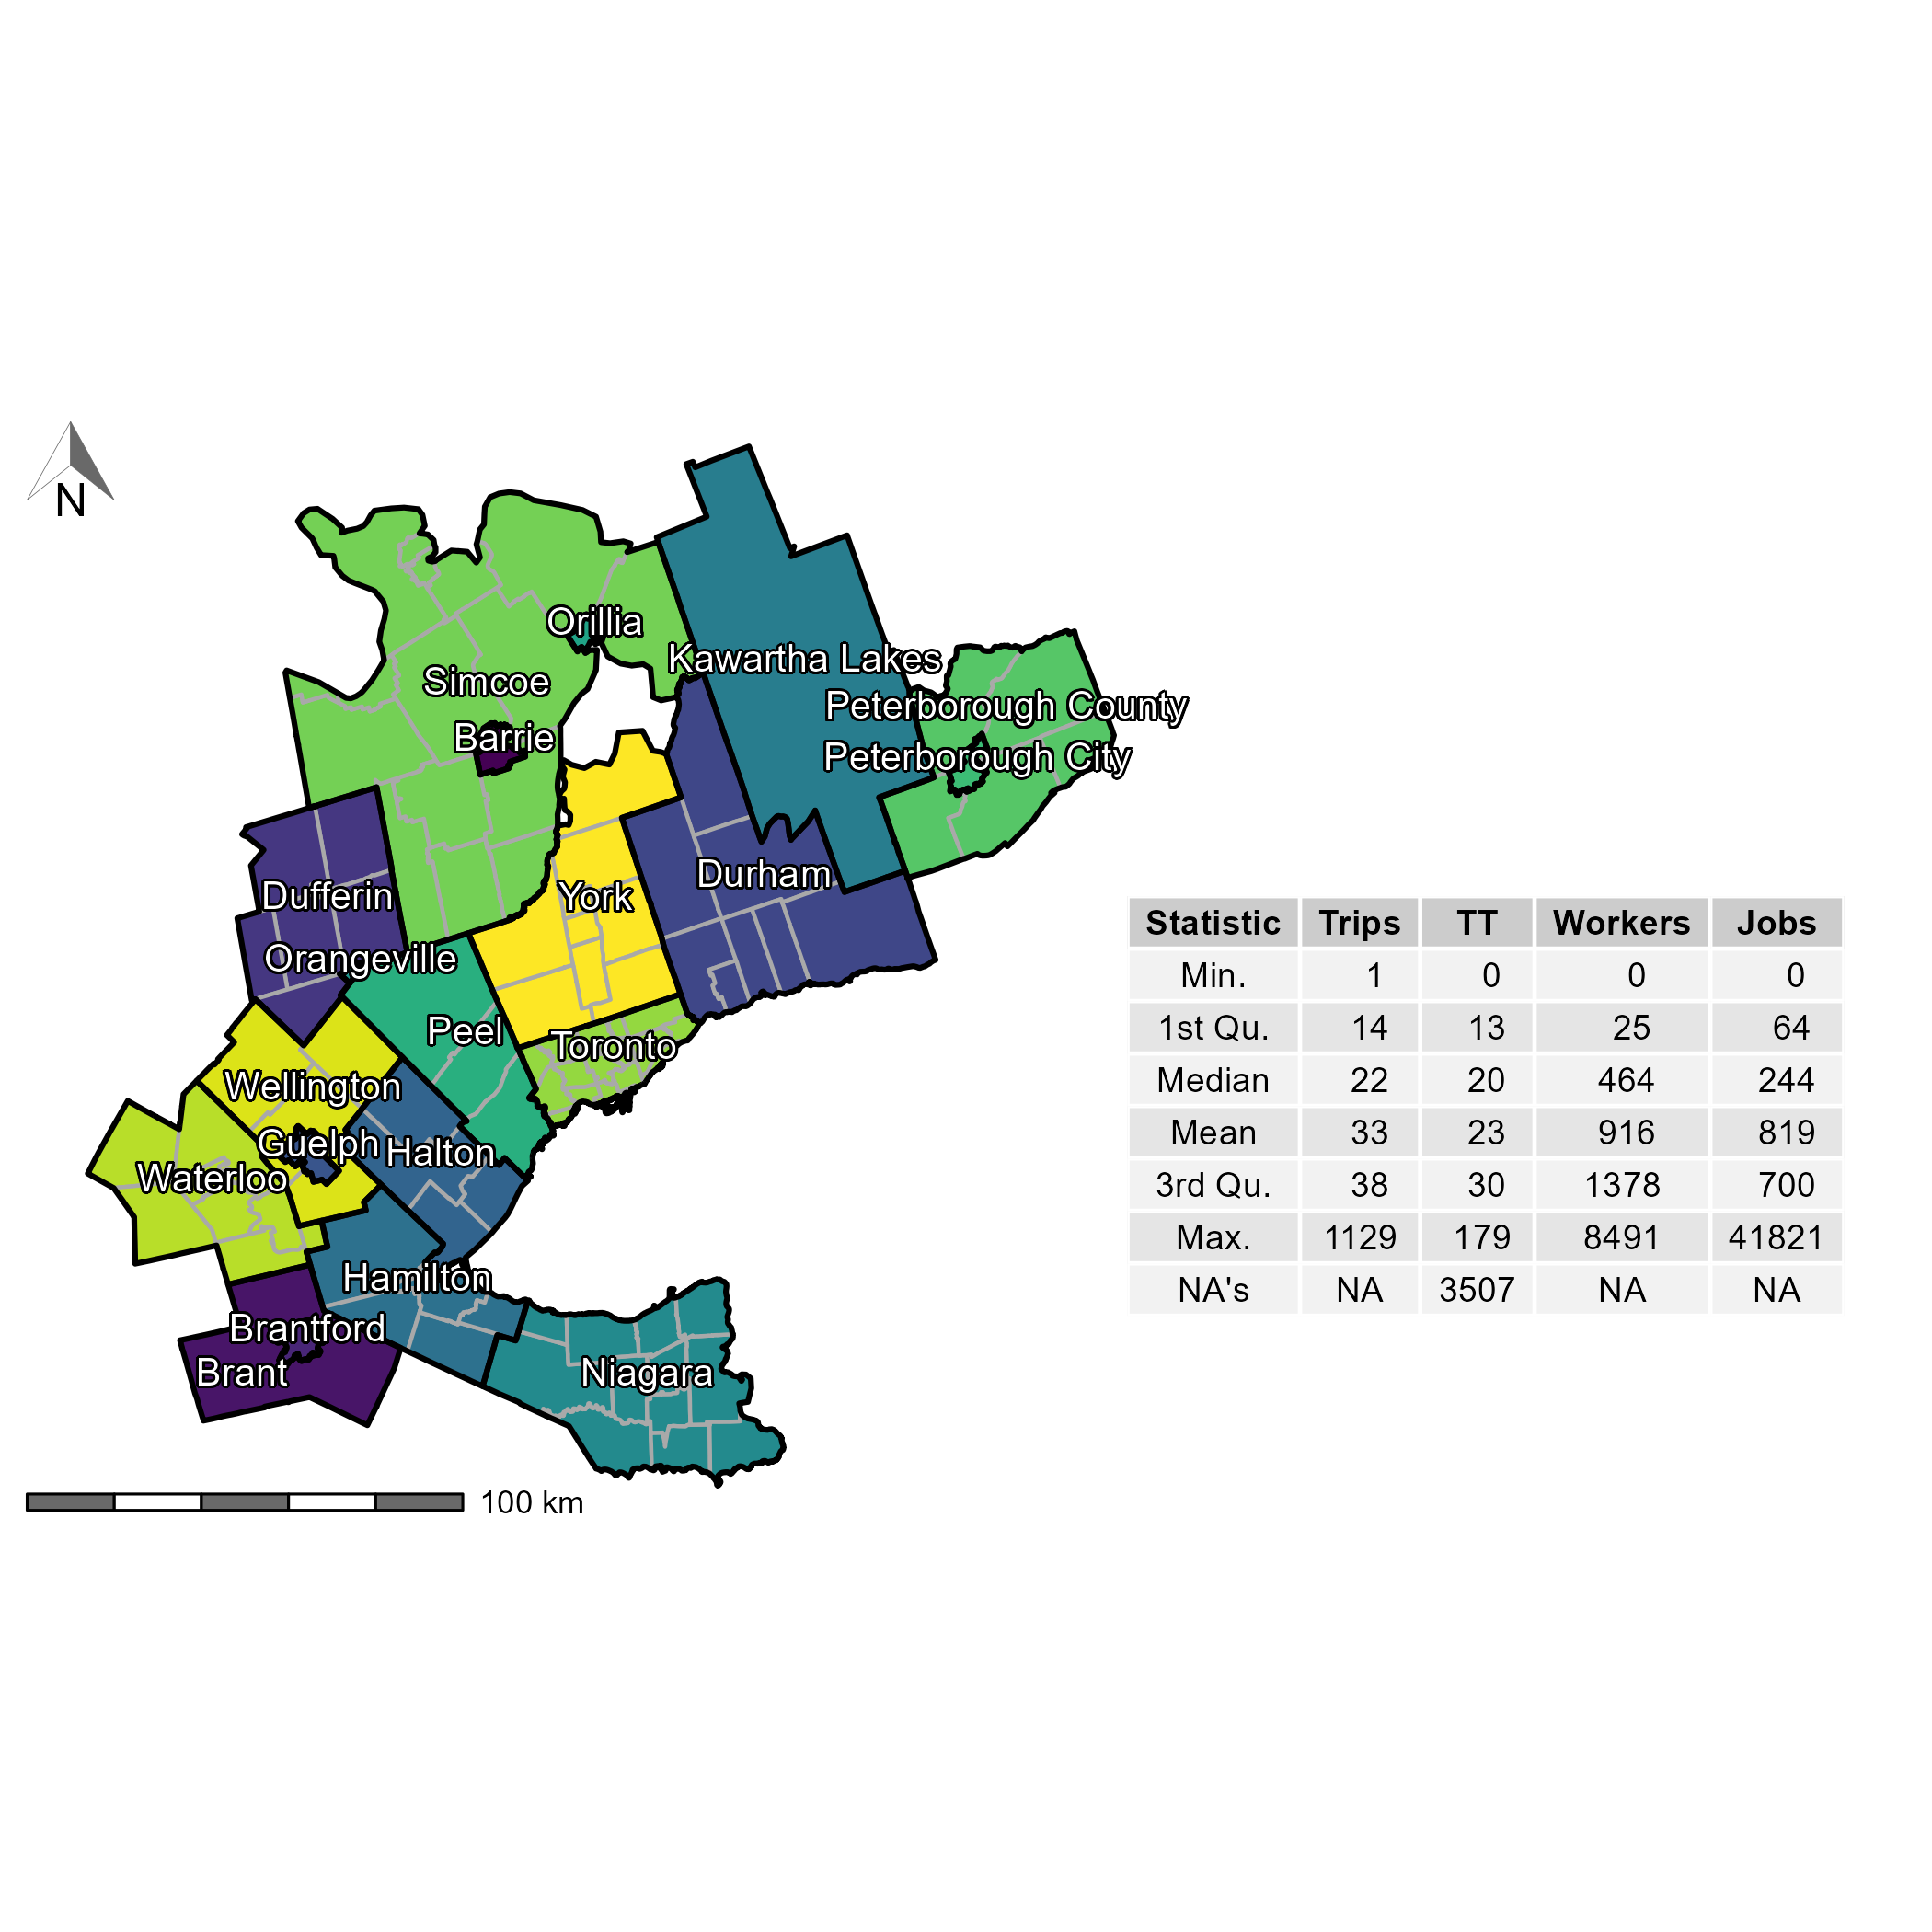
\includegraphics[width=1\linewidth]{images/TTS16-survey-area} 

}

\caption{\label{fig:TTS-16-survey-area}TTS 2016 study area (GGH, Ontario, Canada) along with the descriptive statistics of the trips, calculated origin-destination car travel time (TT), workers per TAZ, and jobs per TAZ. Contains 20 regions (black boundaries) and sub-regions (dark gray boundaries).}\label{fig:TTS-16-survey-area}
\end{figure}

\hypertarget{spatial-employment-characteristics-in-toronto}{%
\subsection{Spatial employment characteristics in
Toronto}\label{spatial-employment-characteristics-in-toronto}}

\begin{figure}
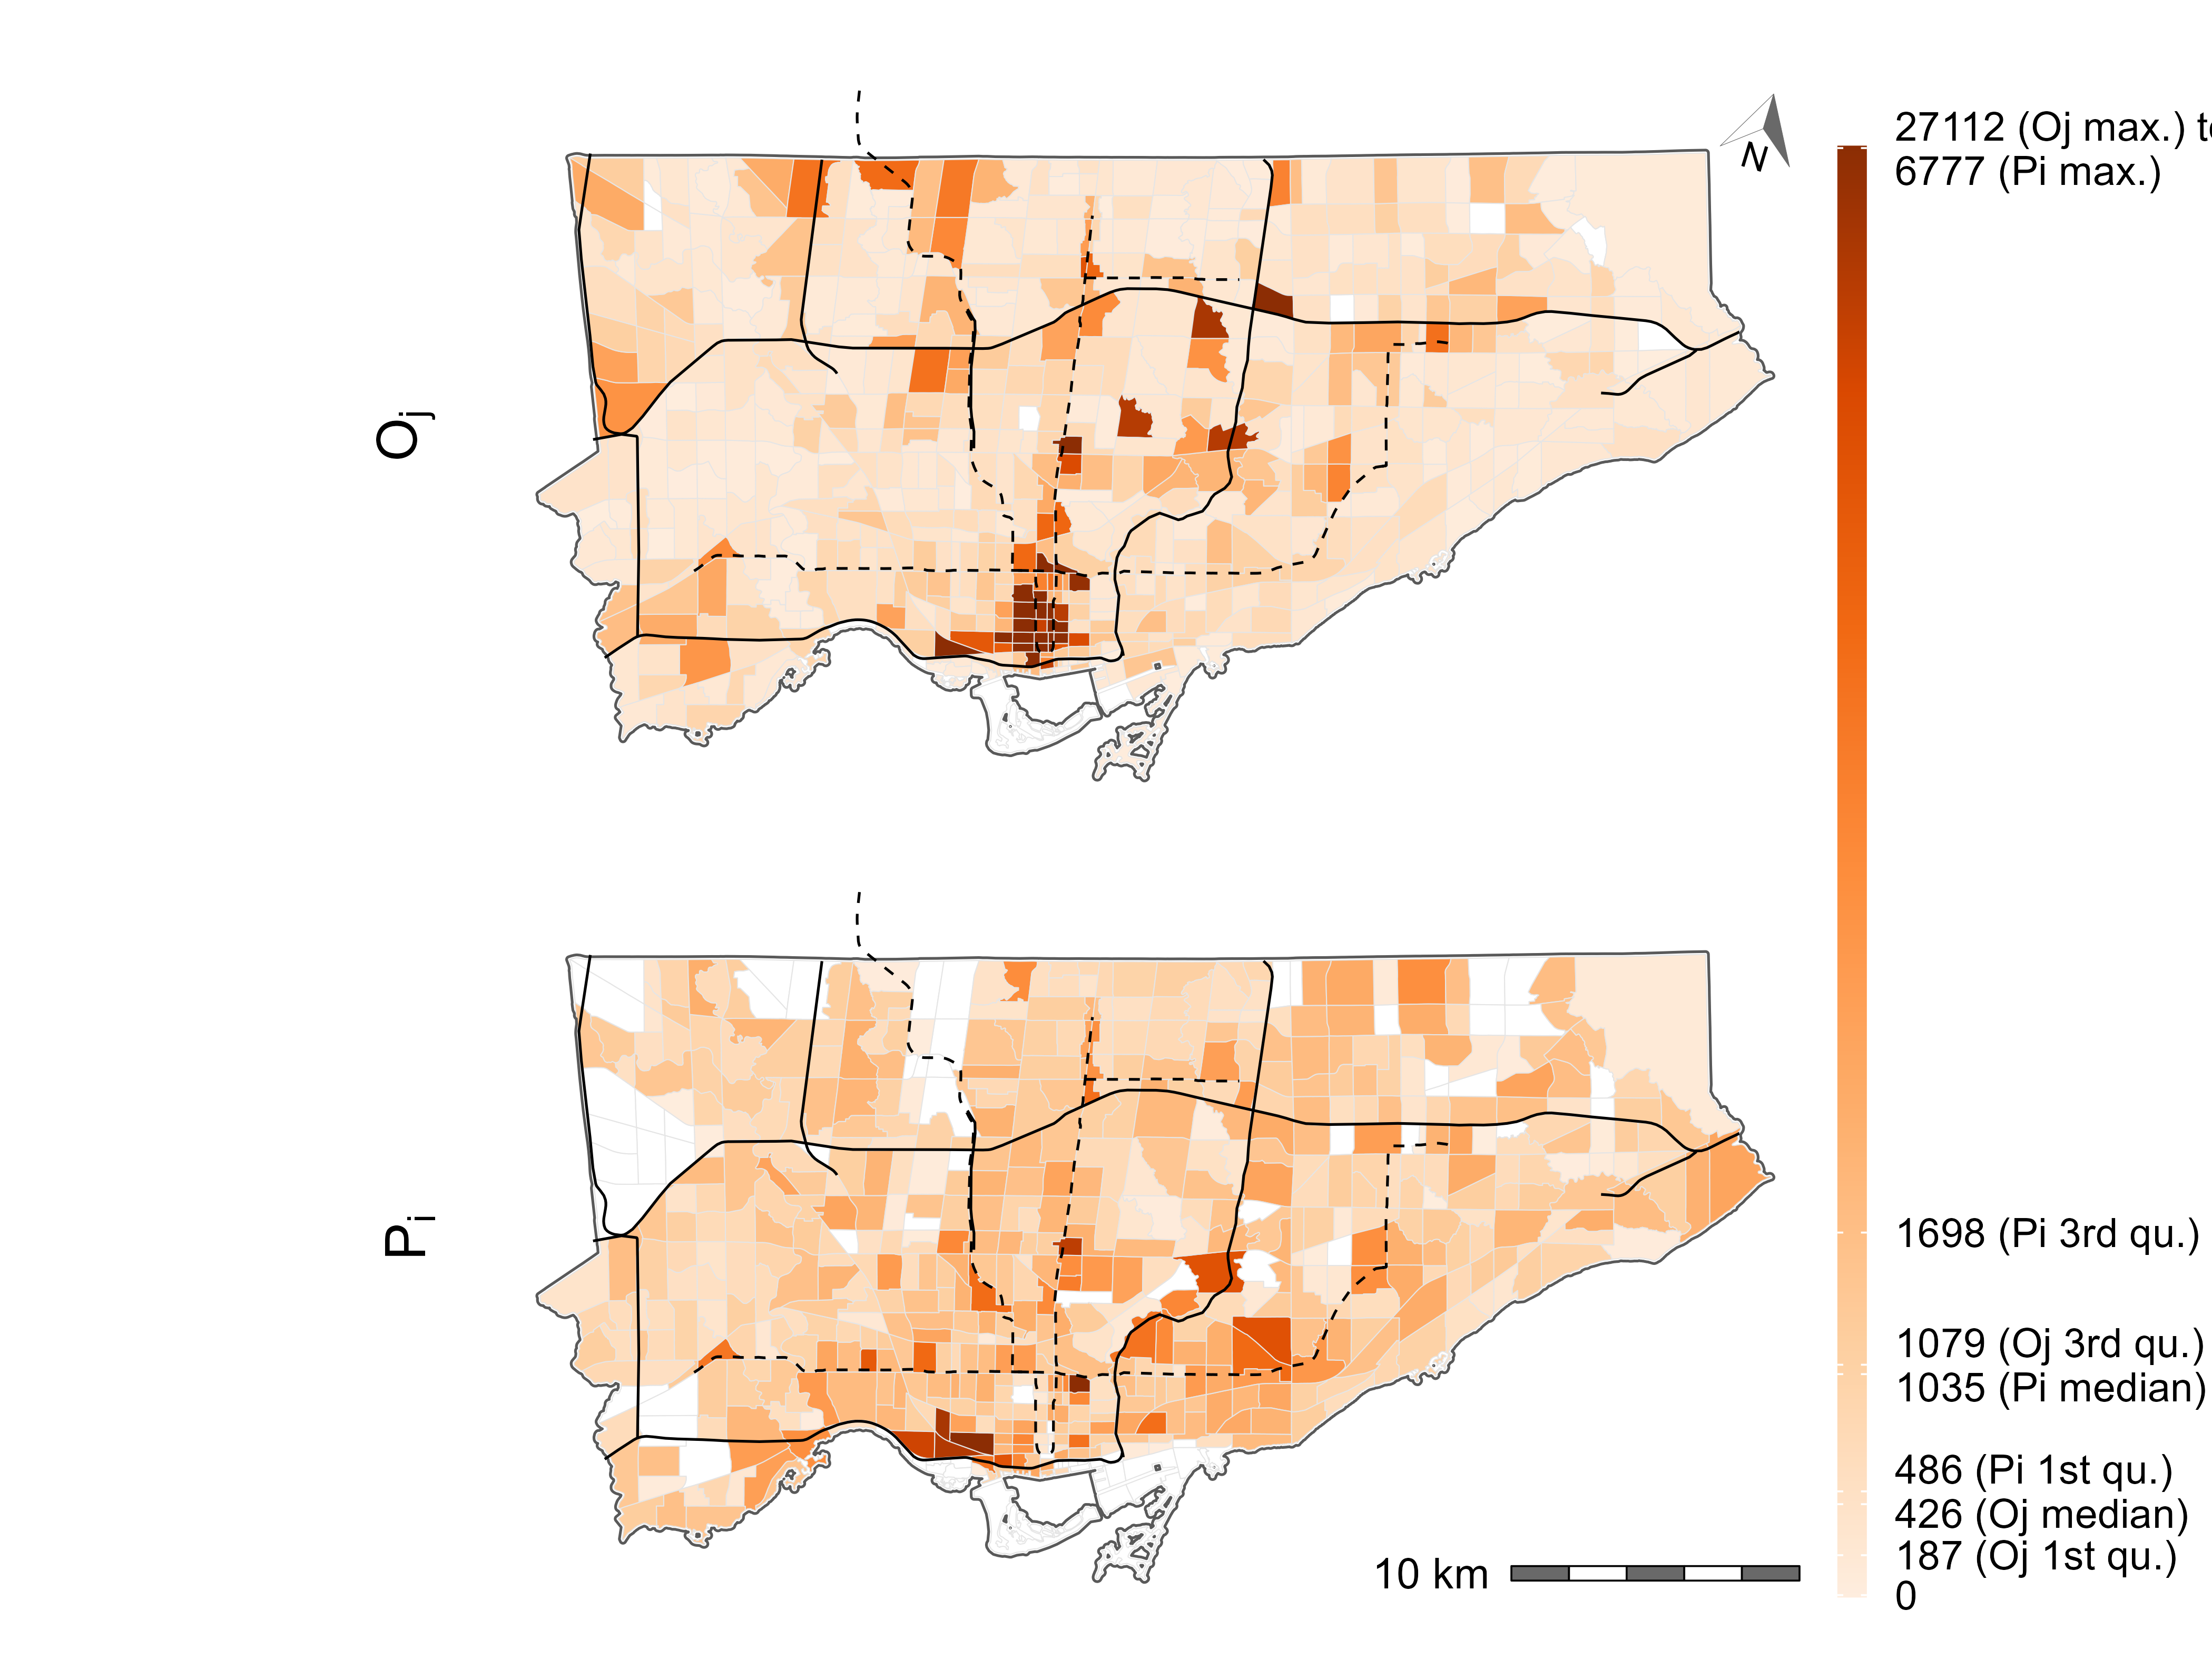
\includegraphics[width=1\linewidth]{images/spatial-dist-jobs-pop-Toronto-plot} \caption{\label{fig:s-dist-Toronto-plot}  Spatial distribution of full-time jobs (top) and full-time working population (bottom) for the city of Toronto as provided by the 2016 TTS. Black lines represent expressways and black dashed lines represent subway lines.}\label{fig:spatial-dist-Toronto-plot}
\end{figure}

\begin{figure}
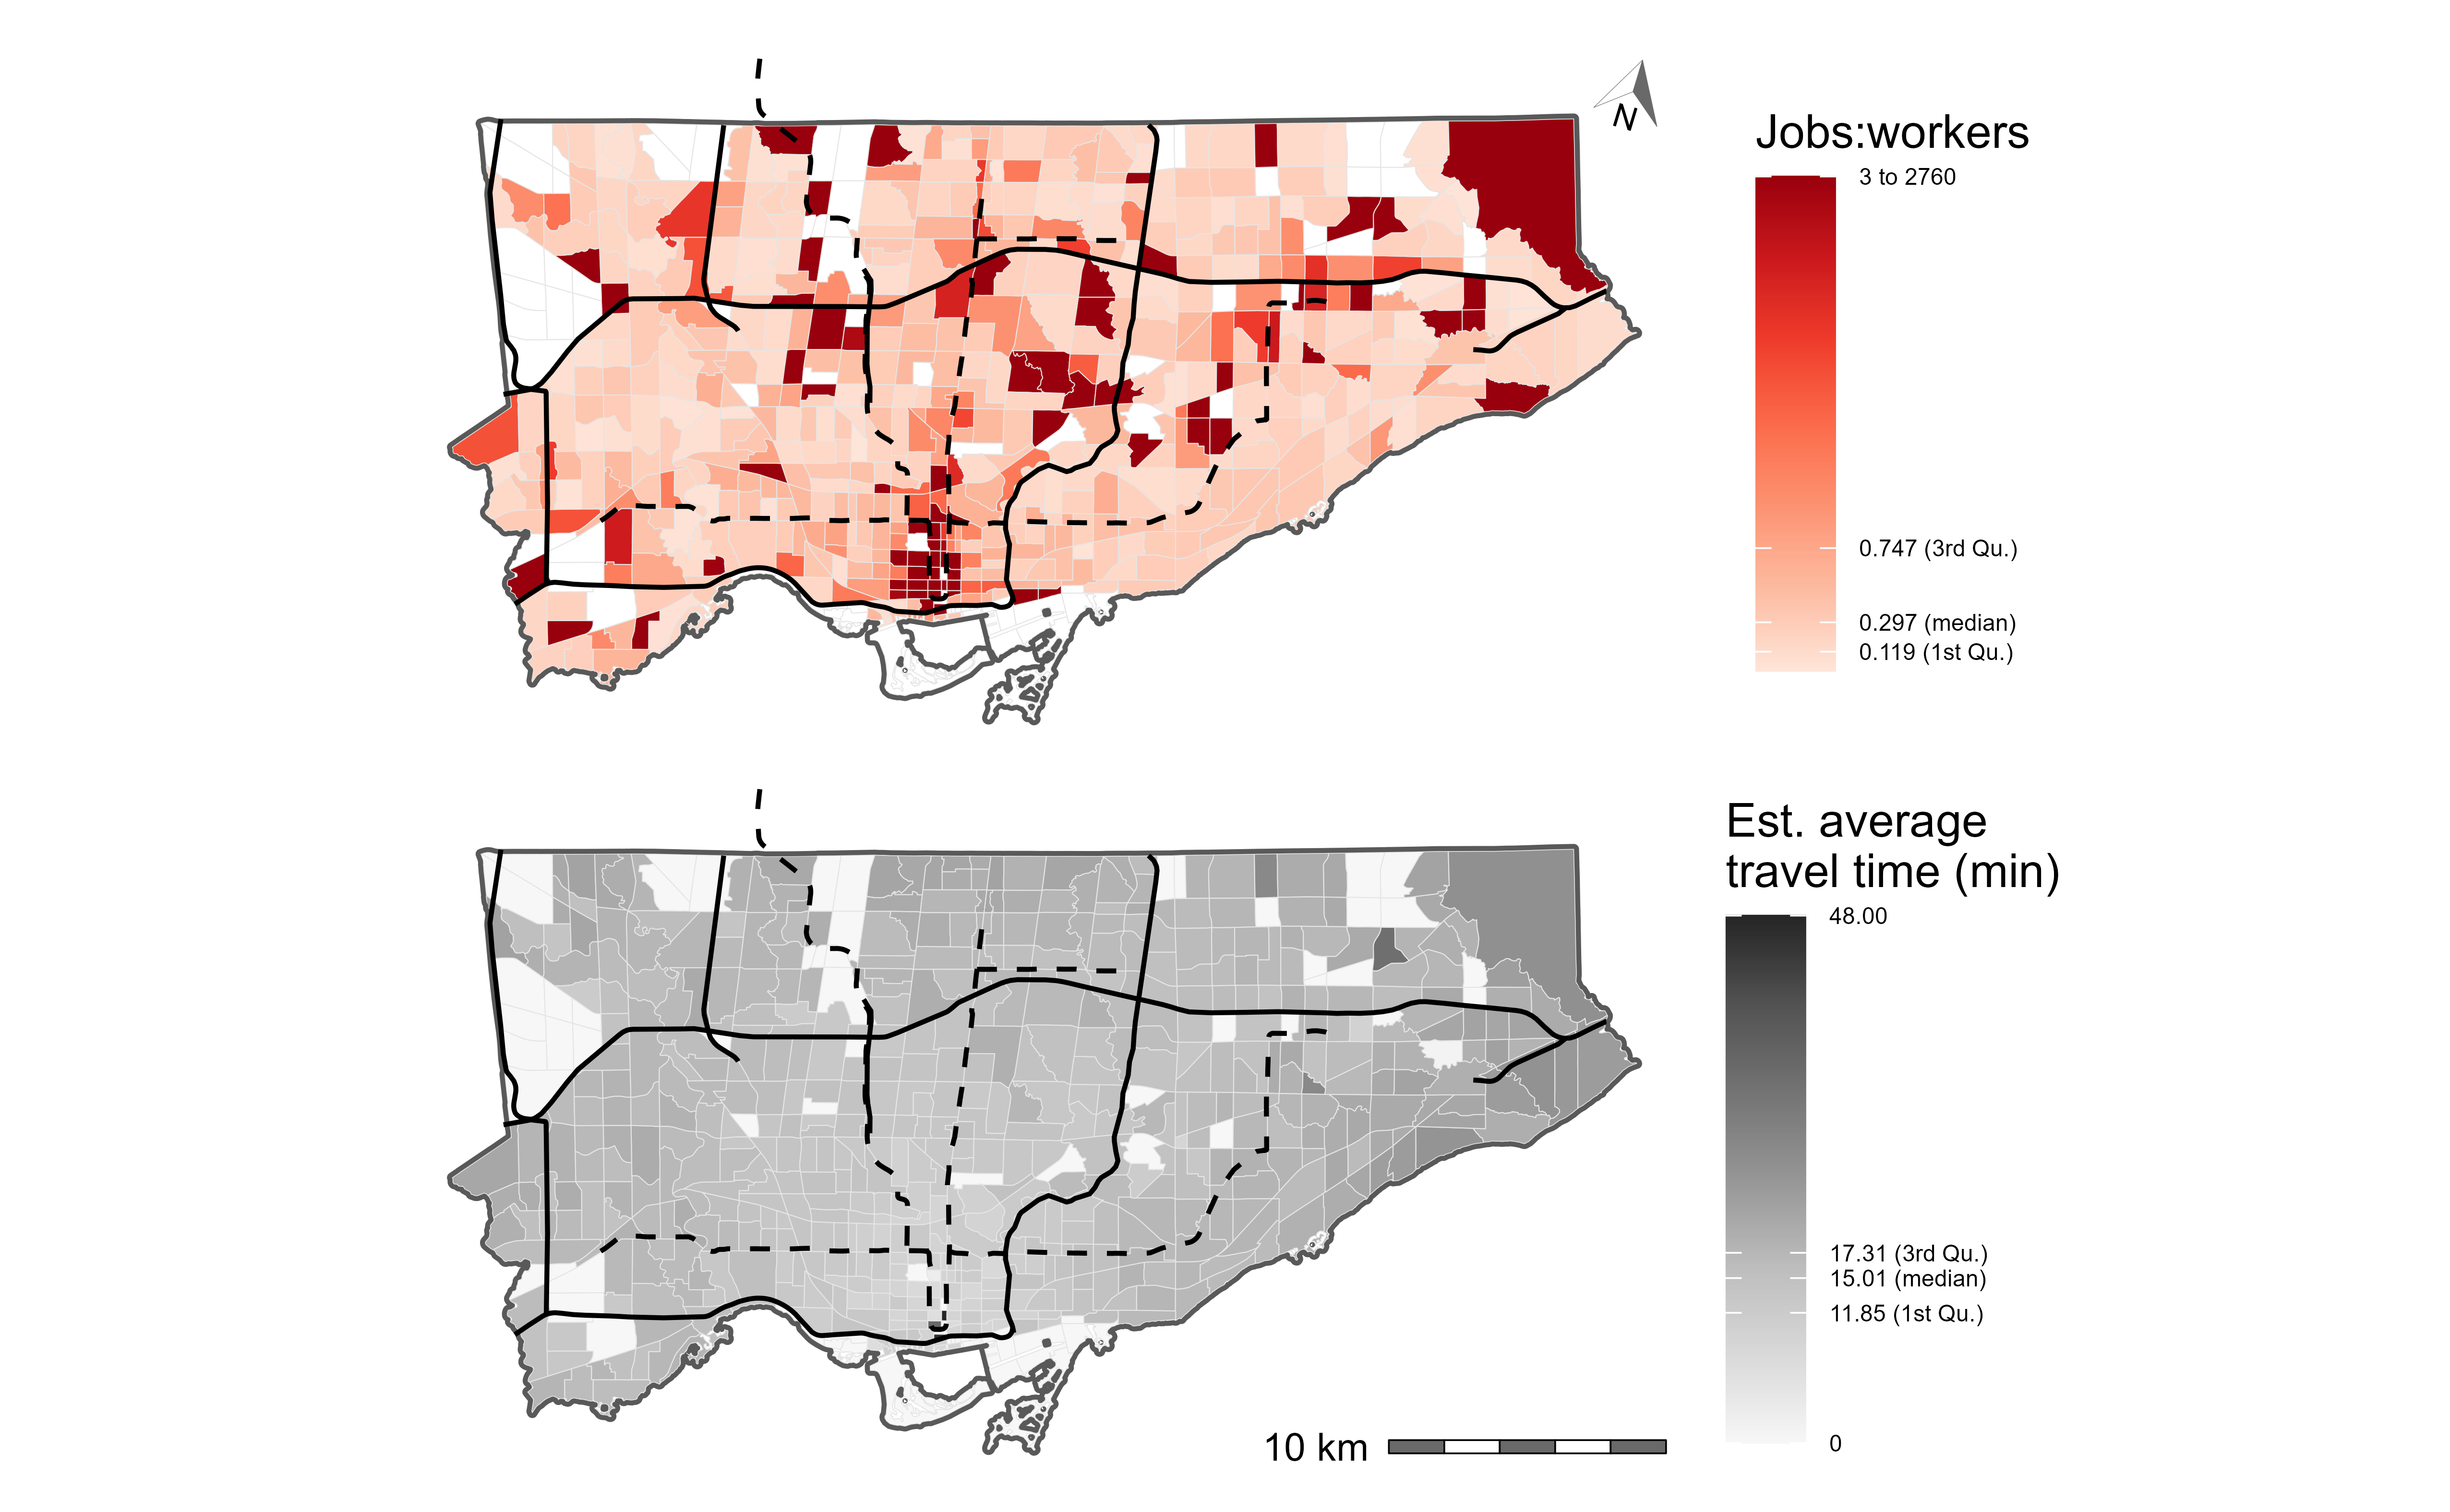
\includegraphics[width=1\linewidth]{images/spatial-dist-jobs-pop-Toronto-plot2} \caption{\label{fig:s-dist-Toronto-plot2}  Spatial distribution of full-time working jobs and worker ratio (top) and car travel time to jobs estimated using R5R for the city of Toronto as provided by the 2016 TTS. Black lines represent expressways and black dashed lines represent subway lines.}\label{fig:spatial-dist-Toronto-plot2}
\end{figure}

As mentioned, the focus of this empirical example is on the city of
Toronto. It is the largest city in the GGH and represents a significant
subset of workers and jobs in the GGH; 22\% of workers in the GGH live
in Toronto and 25\% of jobs are located within Toronto that these
workers take. The spatial distribution of jobs (purple) and workers
(orange) are captured in Figure \ref{fig:s-dist-Toronto-plot}. It can be
seen that a large cluster of jobs can be found in the central southern
part of Toronto (the downtown core). Spatial trends in the distribution
of workers is less apparent relative to the distribution of jobs.

Next, the spatial distribution of the jobs to workers ratio
(jobs:workers) (red) and the estimated car travel time (grey) is
visualized in Figure \ref{fig:s-dist-Toronto-plot2}. Some of the
jobs:workers balance predictably clusters near major transportation
networks (i.e, the north-south subway line and highways) where
surrounding land is more commonly zoned for commercial use. By contrast,
the estimated average travel time to work is more even throughout the
city, with lower travel times within the downtown core and longer travel
times for TAZ located further and further from the core. Interestingly,
travel times in certain TAZ with a high jobs:worker balance occur.

Nonetheless, the point of these visualizations are to demonstrate the
spatial distribution of worker and job data in the city of Toronto to
contextualize spatial availability and Shen- and Hansen- type measures.
Assessing contributing factors to patterns of variable clustering are
outside of the paper's scope and left to further research.

\hypertarget{calibration-of-an-impedance-function-for-toronto}{%
\subsection{Calibration of an impedance function for
Toronto}\label{calibration-of-an-impedance-function-for-toronto}}

In toy example introduced in a preceding section, we used a negative
exponential function with the parameter reported by Shen (1998). For the
empirical Toronto data set, we calibrate an impedance function on the
trip length distribution (TLD) of commute trips. Briefly, a TLD
represents the proportion of trips that are taken at a specific travel
cost (e.g., travel time); this distribution is commonly used to derive
impedance functions in accessibility research (Batista et al., 2019;
Horbachov and Svichynskyi, 2018; Lopez and Paez, 2017).

As mentioned, the calculations are undertaken for the city of Toronto to
facilitate a comparison across measures. As such, only the work-related
trips with origins and destinations within the boundaries of Toronto are
selected. Specifically, edge trips are not included such as trips
originating in Toronto but finishing outside of Toronto and trips
originating outside of Toronto but finishing in Toronto. The empirical
and theoretical TLD for this Toronto data set are represented in the
top-left panel of Figure \ref{fig:TLD-norm-plot}. Maximum likelihood
estimation and the Nelder-Mead method for direct optimization available
within the \{fitdistrplus\} package (Delignette-Muller and Dutang, 2015)
were used. Based on goodness-of-fit criteria and diagnostics the normal
distribution was selected (see Figure \ref{fig:TLD-norm-plot}).

\begin{figure}

{\centering 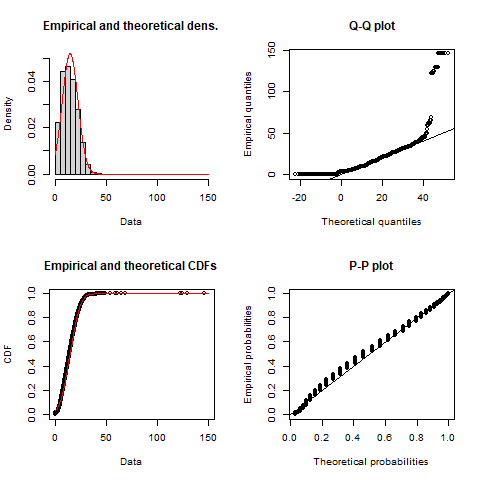
\includegraphics[width=0.8\linewidth]{images/impedance_function} 

}

\caption{\label{fig:TLD-norm-plot}Car trip length distribution and calibrated normal distribution impedance function (red line) with associated Q-Q and P-P plots. Based on TTS 2016.}\label{fig:TLD-norm-plot}
\end{figure}

The normal distribution is defined in Equation (\ref{norm-dist}), where
we see that it depends on a mean parameter \(\mu\) and a standard
deviation parameter \(\sigma\). The estimated values of these parameters
are \(\mu=\) 14.707 and \(\sigma =\) 7.697.

\begin{equation}
\label{norm-dist}
\begin{array}{l} 
f(x) = \frac{1}{\sigma \sqrt{2\pi}}e^{-\frac{1}{2}(\frac{x-\mu}{\sigma})^2}\\
\end{array}
\end{equation}

\[
\frac{1}{\sigma \sqrt{2\pi}}e^{\frac{1}{2}(\frac{x-\mu}{\sigma})^2}
\]

\hypertarget{accessibility-and-spatial-availability-of-jobs-in-toronto}{%
\subsection{Accessibility and spatial availability of jobs in
Toronto}\label{accessibility-and-spatial-availability-of-jobs-in-toronto}}

 
  \providecommand{\huxb}[2]{\arrayrulecolor[RGB]{#1}\global\arrayrulewidth=#2pt}
  \providecommand{\huxvb}[2]{\color[RGB]{#1}\vrule width #2pt}
  \providecommand{\huxtpad}[1]{\rule{0pt}{#1}}
  \providecommand{\huxbpad}[1]{\rule[-#1]{0pt}{#1}}

\begin{table}[ht]
\begin{centerbox}
\begin{threeparttable}
 \label{tab:verify-employment}
\setlength{\tabcolsep}{0pt}
\begin{tabular}{l}


\hhline{>{\huxb{0, 0, 0}{0.4}}-}
\arrayrulecolor{black}

\multicolumn{1}{!{\huxvb{0, 0, 0}{0.4}}r!{\huxvb{0, 0, 0}{0.4}}}{\huxtpad{6pt + 1em}\raggedleft \hspace{6pt} \textbf{jobs} \hspace{6pt}\huxbpad{6pt}} \tabularnewline[-0.5pt]


\hhline{>{\huxb{0, 0, 0}{0.4}}-}
\arrayrulecolor{black}

\multicolumn{1}{!{\huxvb{0, 0, 0}{0.4}}r!{\huxvb{0, 0, 0}{0.4}}}{\cellcolor[RGB]{242, 242, 242}\huxtpad{6pt + 1em}\raggedleft \hspace{6pt} 7.69e+05 \hspace{6pt}\huxbpad{6pt}} \tabularnewline[-0.5pt]


\hhline{>{\huxb{0, 0, 0}{0.4}}-}
\arrayrulecolor{black}
\end{tabular}
\end{threeparttable}\par\end{centerbox}

\end{table}
 

 
  \providecommand{\huxb}[2]{\arrayrulecolor[RGB]{#1}\global\arrayrulewidth=#2pt}
  \providecommand{\huxvb}[2]{\color[RGB]{#1}\vrule width #2pt}
  \providecommand{\huxtpad}[1]{\rule{0pt}{#1}}
  \providecommand{\huxbpad}[1]{\rule[-#1]{0pt}{#1}}

\begin{table}[ht]
\begin{centerbox}
\begin{threeparttable}
 \label{tab:verify-employment}
\setlength{\tabcolsep}{0pt}
\begin{tabular}{l}


\hhline{>{\huxb{0, 0, 0}{0.4}}-}
\arrayrulecolor{black}

\multicolumn{1}{!{\huxvb{0, 0, 0}{0.4}}r!{\huxvb{0, 0, 0}{0.4}}}{\huxtpad{6pt + 1em}\raggedleft \hspace{6pt} \textbf{jobs} \hspace{6pt}\huxbpad{6pt}} \tabularnewline[-0.5pt]


\hhline{>{\huxb{0, 0, 0}{0.4}}-}
\arrayrulecolor{black}

\multicolumn{1}{!{\huxvb{0, 0, 0}{0.4}}r!{\huxvb{0, 0, 0}{0.4}}}{\cellcolor[RGB]{242, 242, 242}\huxtpad{6pt + 1em}\raggedleft \hspace{6pt} 7.69e+05 \hspace{6pt}\huxbpad{6pt}} \tabularnewline[-0.5pt]


\hhline{>{\huxb{0, 0, 0}{0.4}}-}
\arrayrulecolor{black}
\end{tabular}
\end{threeparttable}\par\end{centerbox}

\end{table}
 

 
  \providecommand{\huxb}[2]{\arrayrulecolor[RGB]{#1}\global\arrayrulewidth=#2pt}
  \providecommand{\huxvb}[2]{\color[RGB]{#1}\vrule width #2pt}
  \providecommand{\huxtpad}[1]{\rule{0pt}{#1}}
  \providecommand{\huxbpad}[1]{\rule[-#1]{0pt}{#1}}

\begin{table}[ht]
\begin{centerbox}
\begin{threeparttable}
 \label{tab:verify-population}
\setlength{\tabcolsep}{0pt}
\begin{tabular}{l}


\hhline{>{\huxb{0, 0, 0}{0.4}}-}
\arrayrulecolor{black}

\multicolumn{1}{!{\huxvb{0, 0, 0}{0.4}}r!{\huxvb{0, 0, 0}{0.4}}}{\huxtpad{6pt + 1em}\raggedleft \hspace{6pt} \textbf{workers} \hspace{6pt}\huxbpad{6pt}} \tabularnewline[-0.5pt]


\hhline{>{\huxb{0, 0, 0}{0.4}}-}
\arrayrulecolor{black}

\multicolumn{1}{!{\huxvb{0, 0, 0}{0.4}}r!{\huxvb{0, 0, 0}{0.4}}}{\cellcolor[RGB]{242, 242, 242}\huxtpad{6pt + 1em}\raggedleft \hspace{6pt} 1.14e+06 \hspace{6pt}\huxbpad{6pt}} \tabularnewline[-0.5pt]


\hhline{>{\huxb{0, 0, 0}{0.4}}-}
\arrayrulecolor{black}
\end{tabular}
\end{threeparttable}\par\end{centerbox}

\end{table}
 

 
  \providecommand{\huxb}[2]{\arrayrulecolor[RGB]{#1}\global\arrayrulewidth=#2pt}
  \providecommand{\huxvb}[2]{\color[RGB]{#1}\vrule width #2pt}
  \providecommand{\huxtpad}[1]{\rule{0pt}{#1}}
  \providecommand{\huxbpad}[1]{\rule[-#1]{0pt}{#1}}

\begin{table}[ht]
\begin{centerbox}
\begin{threeparttable}
 \label{tab:verify-population}
\setlength{\tabcolsep}{0pt}
\begin{tabular}{l}


\hhline{>{\huxb{0, 0, 0}{0.4}}-}
\arrayrulecolor{black}

\multicolumn{1}{!{\huxvb{0, 0, 0}{0.4}}r!{\huxvb{0, 0, 0}{0.4}}}{\huxtpad{6pt + 1em}\raggedleft \hspace{6pt} \textbf{workers} \hspace{6pt}\huxbpad{6pt}} \tabularnewline[-0.5pt]


\hhline{>{\huxb{0, 0, 0}{0.4}}-}
\arrayrulecolor{black}

\multicolumn{1}{!{\huxvb{0, 0, 0}{0.4}}r!{\huxvb{0, 0, 0}{0.4}}}{\cellcolor[RGB]{242, 242, 242}\huxtpad{6pt + 1em}\raggedleft \hspace{6pt} 1.98e+06 \hspace{6pt}\huxbpad{6pt}} \tabularnewline[-0.5pt]


\hhline{>{\huxb{0, 0, 0}{0.4}}-}
\arrayrulecolor{black}
\end{tabular}
\end{threeparttable}\par\end{centerbox}

\end{table}
 

 
  \providecommand{\huxb}[2]{\arrayrulecolor[RGB]{#1}\global\arrayrulewidth=#2pt}
  \providecommand{\huxvb}[2]{\color[RGB]{#1}\vrule width #2pt}
  \providecommand{\huxtpad}[1]{\rule{0pt}{#1}}
  \providecommand{\huxbpad}[1]{\rule[-#1]{0pt}{#1}}

\begin{table}[ht]
\begin{centerbox}
\begin{threeparttable}
 \label{tab:verify-population}
\setlength{\tabcolsep}{0pt}
\begin{tabular}{l}


\hhline{>{\huxb{0, 0, 0}{0.4}}-}
\arrayrulecolor{black}

\multicolumn{1}{!{\huxvb{0, 0, 0}{0.4}}r!{\huxvb{0, 0, 0}{0.4}}}{\huxtpad{6pt + 1em}\raggedleft \hspace{6pt} \textbf{workers} \hspace{6pt}\huxbpad{6pt}} \tabularnewline[-0.5pt]


\hhline{>{\huxb{0, 0, 0}{0.4}}-}
\arrayrulecolor{black}

\multicolumn{1}{!{\huxvb{0, 0, 0}{0.4}}r!{\huxvb{0, 0, 0}{0.4}}}{\cellcolor[RGB]{242, 242, 242}\huxtpad{6pt + 1em}\raggedleft \hspace{6pt} 1.33e+06 \hspace{6pt}\huxbpad{6pt}} \tabularnewline[-0.5pt]


\hhline{>{\huxb{0, 0, 0}{0.4}}-}
\arrayrulecolor{black}
\end{tabular}
\end{threeparttable}\par\end{centerbox}

\end{table}
 

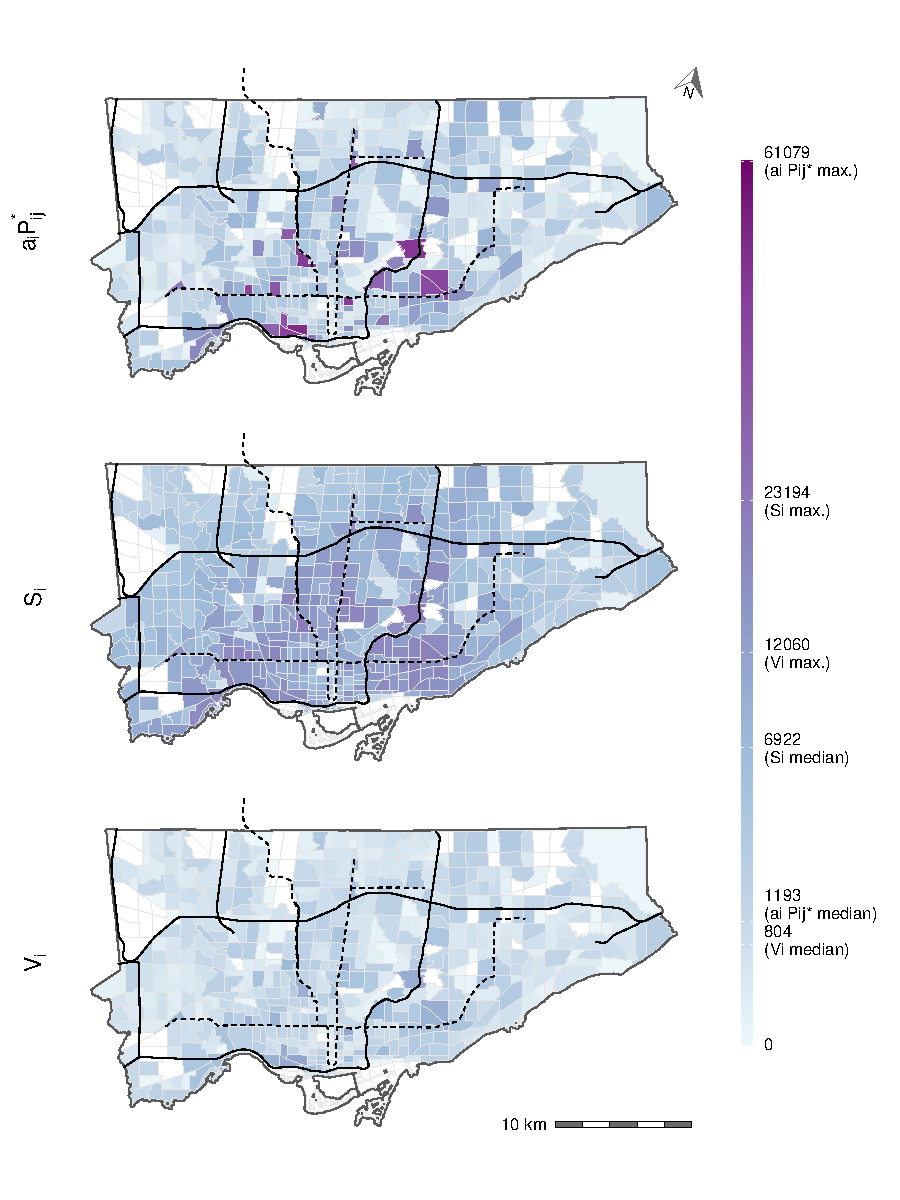
\includegraphics[width=1\linewidth]{Spatial-Availability-Refreshed_files/figure-latex/absolute-accessibility-plot-creation-1}

Figure \ref{fig:absolute-accessibility-plot} contains the absolute
accessibility values in number of jobs accessible using Shen-type
accessibility, Hansen-type accessibility, and the number of jobs
\emph{available} using the spatial availability measure. The Shen-type
accessibility is multiplied by the \emph{effective opportunity-seeking
population} to yield a value that corresponds to absolute number of
accessible jobs (considering competition) according to Shen's
definition. The Hansen-type accessibility is an unconstrained case of
accessibility in which all jobs which are in-reach of each origin
(according to the impedance function); each value corresponds to the
number of jobs which can be reach at each origin assuming no
competition. Lastly, the spatial availability measure is a constrained
case of accessibility which yields the number of jobs, at each origin,
considering competition from the population in nearby origin and the
relative travel cost (according to the impedance function).

The proportional allocation mechanism of spatial availability ensures
that the job availability value for each origin all sums to the
city-wide total of 769,231 jobs (i.e., the number of destination flows
from Toronto origins to Toronto destinations). The regional total for
Hansen-type accessibility is 4,318,005 jobs, which as a value is
practically meaningless since the measure is unconstrained; it
represents the sum of opportunities that have been counted anywhere from
1 to many times depending on the impedance function. As previously
discussed, unconstrained counting of the same opportunity by all origins
is not an issue if the opportunity itself is non-exclusive, but since
one origin-to-destination full-time employment trip corresponds to 1 job
and 1 worker, it is inappropriate to use unconstrained measures to
capture employment characteristics. Though, using unconstrained
Hansen-style measure for employment data can depicted urban form but
applications to create actionable policy is lacking .

On a similar note to Hasen-type, the \emph{absolute} Shen-type measure
(as understood by Shen's definition of \(P_i\) being equal to
\(P_{ij}^*\) sums to the city-wide value of 2,064,055 jobs; this value
demonstrates how the Shen-type measure that is presented a rate (i.e.,
opportunities per capita) can be misunderstood and multiplied by the
\emph{effective opportunity-seeking population} (i.e., the denominator
of the rate \(P_{ij}^*\)) to express an absolute accessibility score.
The misleading interpretation of confounding \(P_i\) with \(P_{ij}^*\)
yields an \emph{incorrect} competitively accessible job values because
\(P_{ij}^*\) greatly exceeds greatly exceeds the city-wide total of
workers (i.e., Toronto origin trips). To the authors' knowledge,
Shen-type accessibility has not been converted to the absolute value in
the way demonstrated within this paper perhaps potentially because the
values are incorrect since Shen's proof (Shen (1998) footnote) does not
hold true. However, we also have not seen the Shen-type measure
converted from the opportunities per capita score to absolute
opportunities, we suspect, because of the ambiguous definition which
conflates \(P_{ij}^*\) with \(P_i\). If \(a_i\) is multiplied by
\(P_i\), it yields the same value as \(V_i\), but, since the definition
of Shen-type measure is equivocal doing so is not clear since the
denominator of \(a_i\) (which is a rate) is \emph{not} \(P_i\).

 
  \providecommand{\huxb}[2]{\arrayrulecolor[RGB]{#1}\global\arrayrulewidth=#2pt}
  \providecommand{\huxvb}[2]{\color[RGB]{#1}\vrule width #2pt}
  \providecommand{\huxtpad}[1]{\rule{0pt}{#1}}
  \providecommand{\huxbpad}[1]{\rule[-#1]{0pt}{#1}}

\begin{table}[ht]
\begin{centerbox}
\begin{threeparttable}
 \label{tab:unnamed-chunk-3}
\setlength{\tabcolsep}{0pt}
\begin{tabular}{l l}


\hhline{>{\huxb{0, 0, 0}{0.4}}->{\huxb{0, 0, 0}{0.4}}-}
\arrayrulecolor{black}

\multicolumn{1}{!{\huxvb{0, 0, 0}{0.4}}r!{\huxvb{0, 0, 0}{0}}}{\huxtpad{6pt + 1em}\raggedleft \hspace{6pt} \textbf{osp} \hspace{6pt}\huxbpad{6pt}} &
\multicolumn{1}{r!{\huxvb{0, 0, 0}{0.4}}}{\huxtpad{6pt + 1em}\raggedleft \hspace{6pt} \textbf{total\_workers} \hspace{6pt}\huxbpad{6pt}} \tabularnewline[-0.5pt]


\hhline{>{\huxb{0, 0, 0}{0.4}}->{\huxb{0, 0, 0}{0.4}}-}
\arrayrulecolor{black}

\multicolumn{1}{!{\huxvb{0, 0, 0}{0.4}}r!{\huxvb{0, 0, 0}{0}}}{\cellcolor[RGB]{242, 242, 242}\huxtpad{6pt + 1em}\raggedleft \hspace{6pt} 1.73e+06 \hspace{6pt}\huxbpad{6pt}} &
\multicolumn{1}{r!{\huxvb{0, 0, 0}{0.4}}}{\cellcolor[RGB]{242, 242, 242}\huxtpad{6pt + 1em}\raggedleft \hspace{6pt} 7.69e+05 \hspace{6pt}\huxbpad{6pt}} \tabularnewline[-0.5pt]


\hhline{>{\huxb{0, 0, 0}{0.4}}->{\huxb{0, 0, 0}{0.4}}-}
\arrayrulecolor{black}
\end{tabular}
\end{threeparttable}\par\end{centerbox}

\end{table}
 

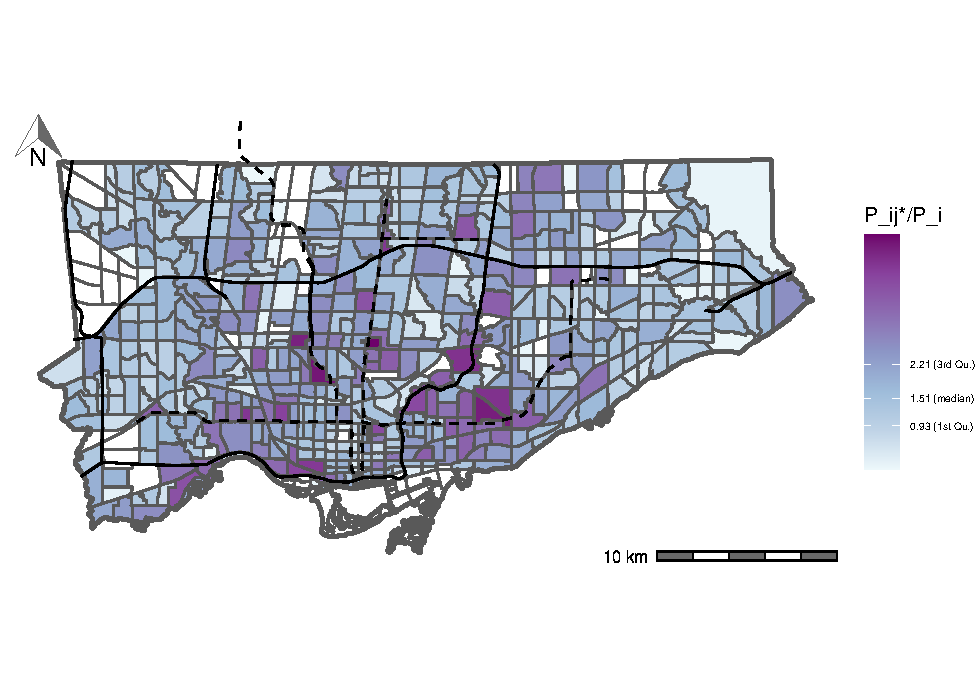
\includegraphics[width=1\linewidth]{Spatial-Availability-Refreshed_files/figure-latex/ratio-OPS-to-pop-plot-creation-1}

\begin{figure}
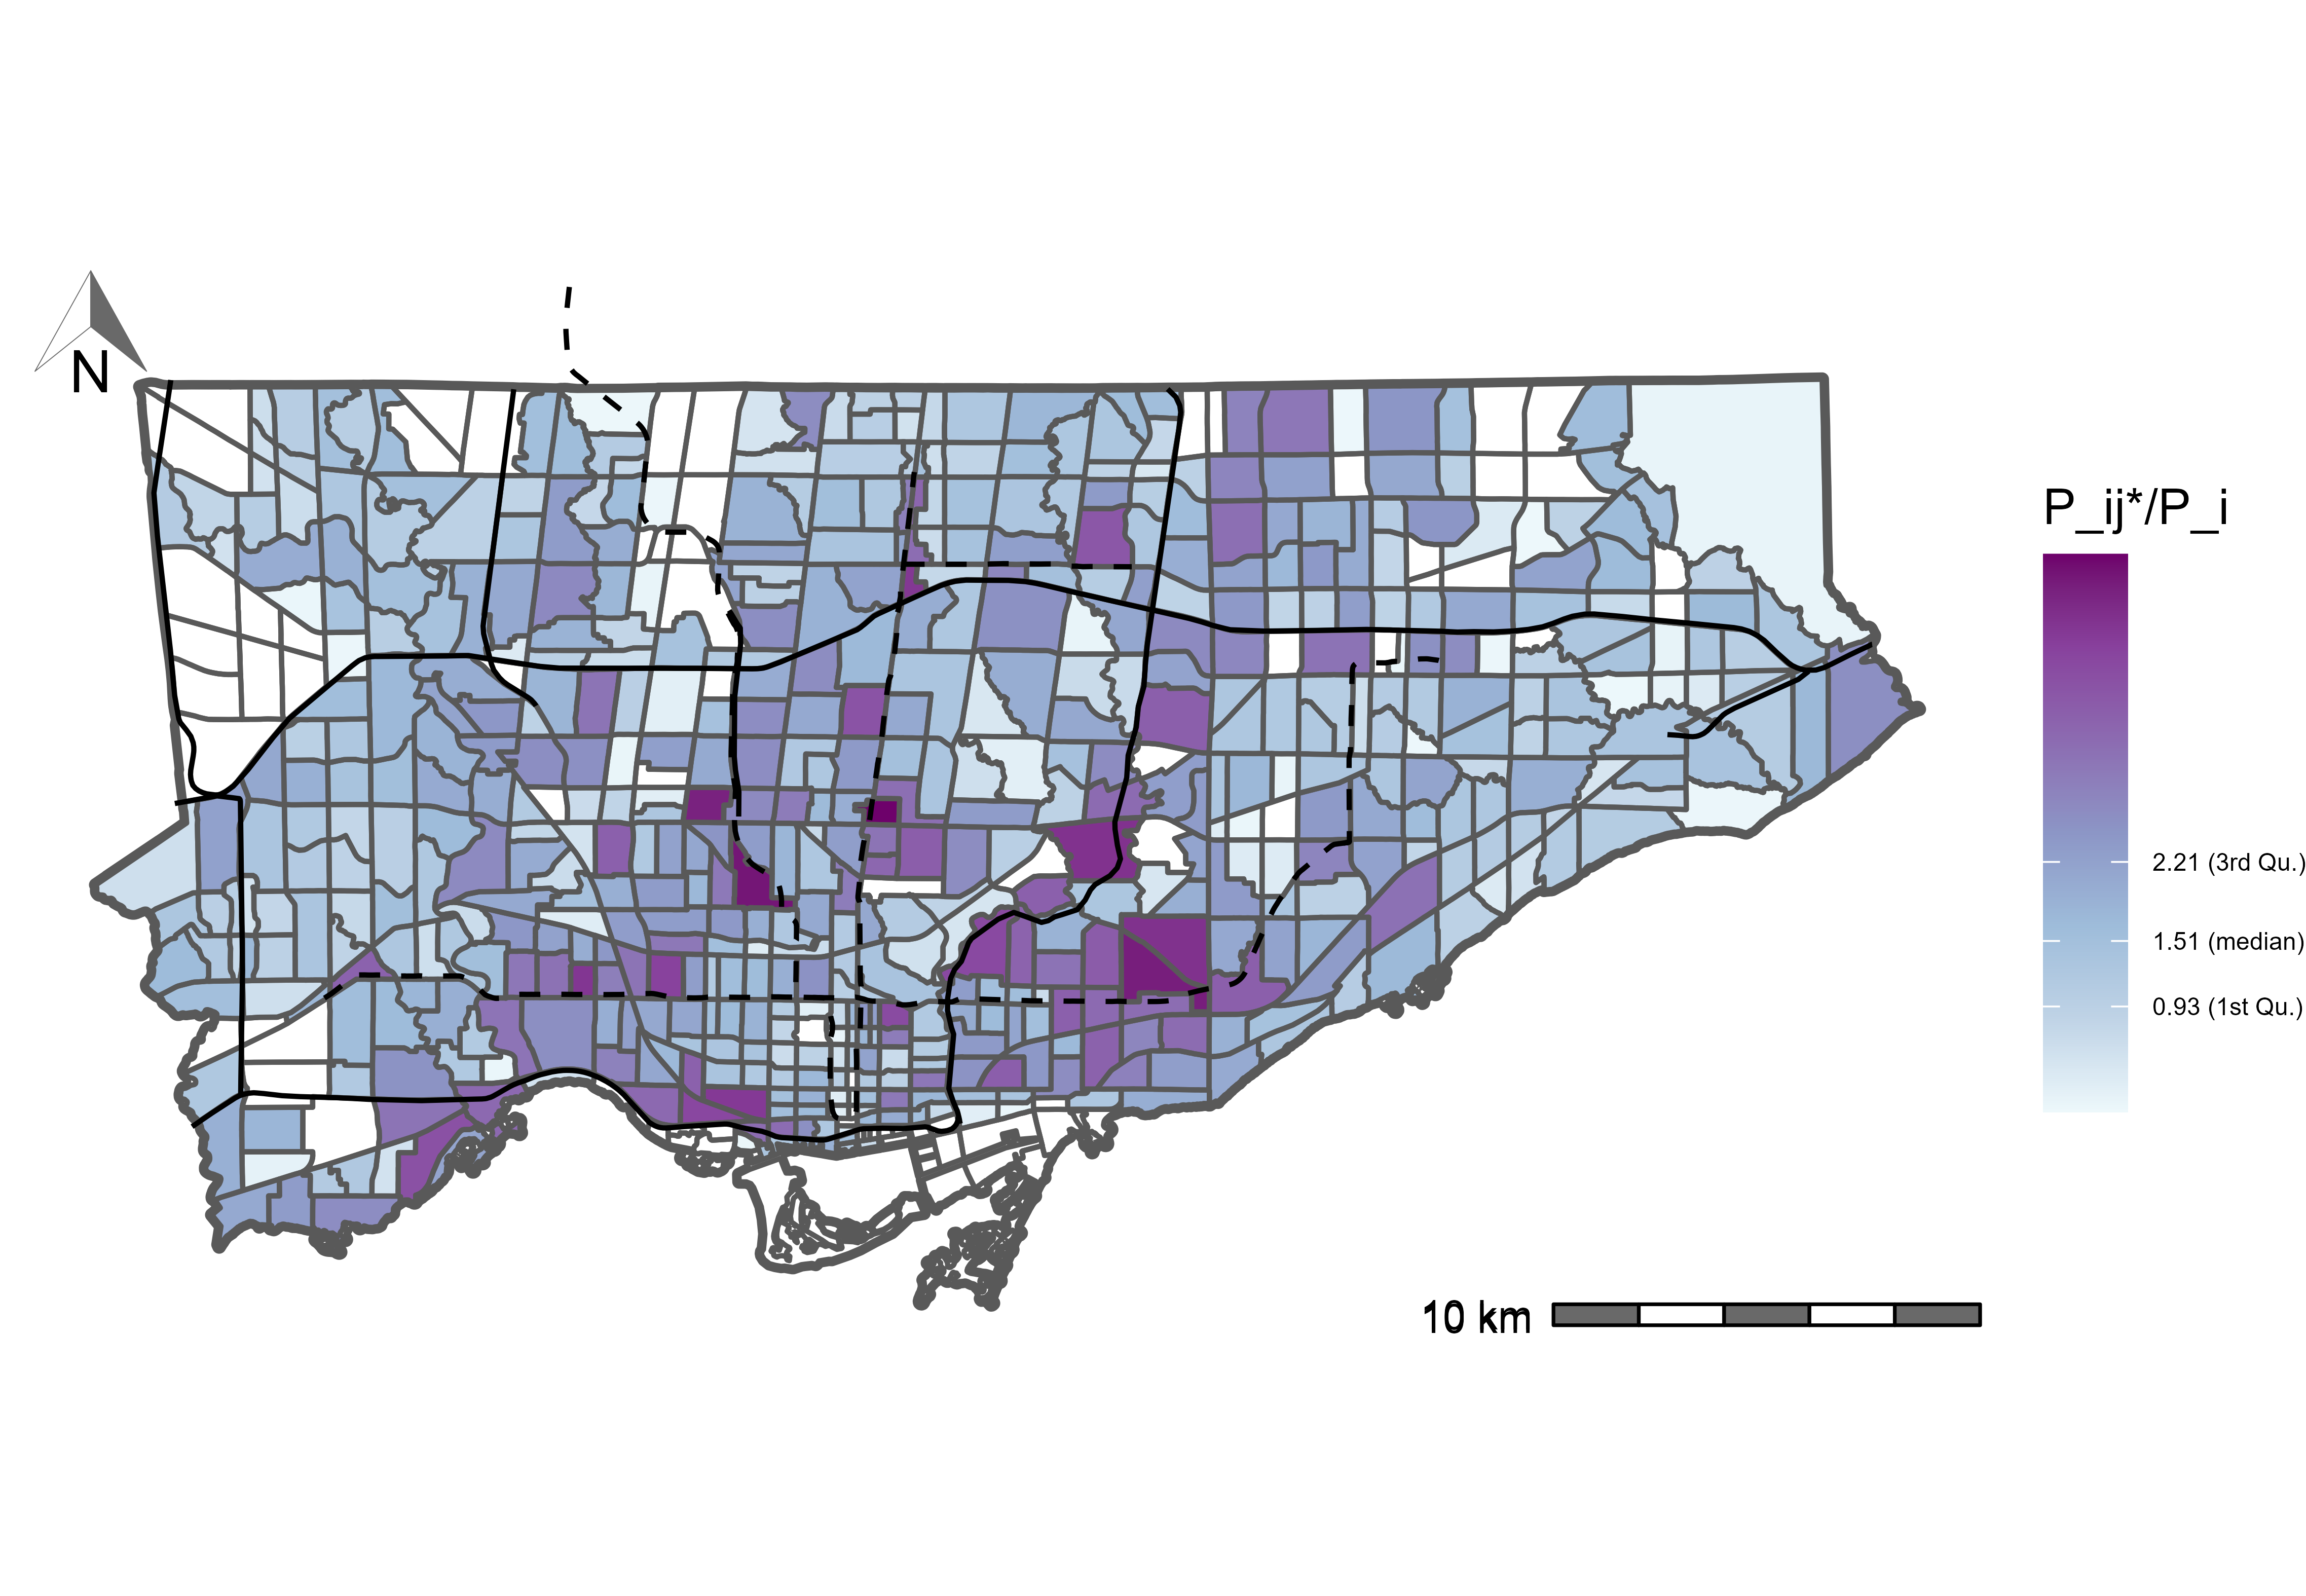
\includegraphics[width=1\linewidth]{images/osp_plot_TO} \caption{\label{fig:ratio-OPS-to-pop-plot}  The ratio of the effective opportunity seeking population to the population in Toronto. Black lines represent expressways and black dashed lines represent subway lines.}\label{fig:ratio-OPS-to-pop-plot}
\end{figure}

It is important to understand the difference between \(P_i\) and
\(P_{ij}^*\) since their impacts is not the same across space. See
Figure \ref{fig:ratio-OPS-to-pop-plot} which presents the ratio of
\(P_{ij}^*\) to \(P_i\) which presents how this effect is not constant
across space. As a consequence of the inflated population (i.e.,
\(P_{ij}^*\) \textgreater{} \(P_i\)), if attempting to calculate impacts
associated with Shen-type measure (absolute value) such as the city-wide
travel time, you can see how the travel time is exaggerated by the
Shen-type measure. Consequently, when using spatial availability
(recall: this equal to \(a_i\) multiplied by \(P_i\)) which sums to the
\emph{total} number of jobs in the city, the travel time can be
accuratedly calculated (as accurately as the input data).

 
  \providecommand{\huxb}[2]{\arrayrulecolor[RGB]{#1}\global\arrayrulewidth=#2pt}
  \providecommand{\huxvb}[2]{\color[RGB]{#1}\vrule width #2pt}
  \providecommand{\huxtpad}[1]{\rule{0pt}{#1}}
  \providecommand{\huxbpad}[1]{\rule[-#1]{0pt}{#1}}

\begin{table}[ht]
\begin{centerbox}
\begin{threeparttable}
 \label{tab:unnamed-chunk-4}
\setlength{\tabcolsep}{0pt}
\begin{tabular}{l}


\hhline{>{\huxb{0, 0, 0}{0.4}}-}
\arrayrulecolor{black}

\multicolumn{1}{!{\huxvb{0, 0, 0}{0.4}}l!{\huxvb{0, 0, 0}{0.4}}}{\huxtpad{6pt + 1em}\raggedright \hspace{6pt} \textbf{total\_travel\_time} \hspace{6pt}\huxbpad{6pt}} \tabularnewline[-0.5pt]


\hhline{>{\huxb{0, 0, 0}{0.4}}-}
\arrayrulecolor{black}

\multicolumn{1}{!{\huxvb{0, 0, 0}{0.4}}l!{\huxvb{0, 0, 0}{0.4}}}{\cellcolor[RGB]{242, 242, 242}\huxtpad{6pt + 1em}\raggedright \hspace{6pt} 497258.183377296 \hspace{6pt}\huxbpad{6pt}} \tabularnewline[-0.5pt]


\hhline{>{\huxb{0, 0, 0}{0.4}}-}
\arrayrulecolor{black}
\end{tabular}
\end{threeparttable}\par\end{centerbox}

\end{table}
 

 
  \providecommand{\huxb}[2]{\arrayrulecolor[RGB]{#1}\global\arrayrulewidth=#2pt}
  \providecommand{\huxvb}[2]{\color[RGB]{#1}\vrule width #2pt}
  \providecommand{\huxtpad}[1]{\rule{0pt}{#1}}
  \providecommand{\huxbpad}[1]{\rule[-#1]{0pt}{#1}}

\begin{table}[ht]
\begin{centerbox}
\begin{threeparttable}
 \label{tab:unnamed-chunk-4}
\setlength{\tabcolsep}{0pt}
\begin{tabular}{l}


\hhline{>{\huxb{0, 0, 0}{0.4}}-}
\arrayrulecolor{black}

\multicolumn{1}{!{\huxvb{0, 0, 0}{0.4}}l!{\huxvb{0, 0, 0}{0.4}}}{\huxtpad{6pt + 1em}\raggedright \hspace{6pt} \textbf{total\_travel\_time} \hspace{6pt}\huxbpad{6pt}} \tabularnewline[-0.5pt]


\hhline{>{\huxb{0, 0, 0}{0.4}}-}
\arrayrulecolor{black}

\multicolumn{1}{!{\huxvb{0, 0, 0}{0.4}}l!{\huxvb{0, 0, 0}{0.4}}}{\cellcolor[RGB]{242, 242, 242}\huxtpad{6pt + 1em}\raggedright \hspace{6pt} 187393.373611765 \hspace{6pt}\huxbpad{6pt}} \tabularnewline[-0.5pt]


\hhline{>{\huxb{0, 0, 0}{0.4}}-}
\arrayrulecolor{black}
\end{tabular}
\end{threeparttable}\par\end{centerbox}

\end{table}
 

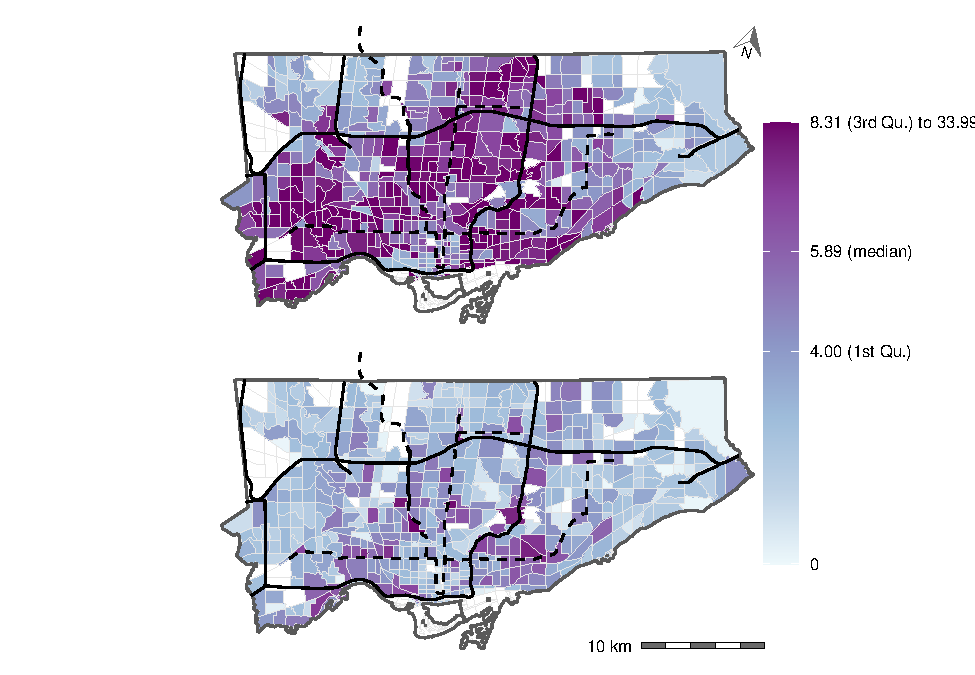
\includegraphics[width=1\linewidth]{Spatial-Availability-Refreshed_files/figure-latex/rate-accessibility-plot-creation-1}

Spatial availability untangles Shen-stype measure so an absolute value
of \emph{opportunity availability} is expressed. Because the
proportional allocation mechanism makes clear that all the opportunities
are being allocated proportionally to all the origins, it makes the
interpretation more clear. It thus can be directly divided by origin
population and expressed as an opportunities per capita score.
Coincidentally, as mentioned, this score is equal to Shen-type measure,
but with a renewed interpretability. When normalized spatial
availability is compared to Hansen-type measure, normalizing the output
by population directly is unique; spatial availability can be normalized
by opportunities without the issue of multiple counting of opportunities
which obscures accessibility's meaning. See Figure
\ref{fig:rate-accessibility-plot} which displays the normalized
opportunity per capita spatial availability score and plainly
normalizing Hansen-type accessibility by dividing each value by the
origin population.

\newpage

\hypertarget{conclusions}{%
\section{Conclusions}\label{conclusions}}

Why do differences between Hansen-style measure and the interpretation
of Shen-type measure matter? Because of equity analysis and policy
planning! With spatial availability, we can push accessibility analysis
forward by making it more interpretable. As discussed, Hansen-style
accessibility value cannot be interpreted directly in either form
(though it can be interpreted relatively to speak about urban form). By
contrast, spatial availability yields the number of jobs available
directly.

This property and understanding spatial availability (along with Shen's
accessibility with competition and 2SFCA) as a singly-constrained
measure are important to understanding how accessibility measures can be
broadled interepted. The following are recommendations:

\begin{enumerate}
\def\labelenumi{\arabic{enumi})}
\tightlist
\item
  The Hansen-style accessibilty should be used when opportunities are
  non-exclusive. When opportunities are perfectly exclusive (i.e., 1
  spot for 1 person), spatial availability (i.e., accessibility with
  competition) should be used.
\item
  Though outside of scope, when opportunities are perfectly exclusive ad
  -We argue that spatial availability should be used
\end{enumerate}

\begin{itemize}
\tightlist
\item
  some literature which uses Shen focuses on how travel cost discounts
  job supply (opportunities) and demand (opportunity-seeking
  population). This gets close to disentangling which population
  \emph{effectively} seeking opportunities - but comparing it to the
  population which doesn't seek opportunities has not been made, to the
  authors opportunity. This is critical for equity analysis; i.e., which
  populations can't seek opportunities because of friction of distance?
  This can be plainly seen by seeing the proportion of population, in
  spatial availability, which is allocated to the origin
\end{itemize}

\hypertarget{appendix-a}{%
\section{Appendix A}\label{appendix-a}}

Equivalence of Shen-type accessibility and spatial availability

Population allocation factor:

\[
F^p_{ij} = \frac{P_{i\in r}^\alpha}{\sum_{i}^K P_{i\in r}^\alpha}
\]

\[
F^p_{A} = \frac{P_{A}^\alpha}{P_{A}^\alpha + P_{B}^\alpha + P_{C}^\alpha}
\]

Cost allocation factor:

\[
F^c_{ij} = \frac{f(c_{ij})}{\sum_{i=A}^K f(c_{ij})}
\]

\[
F^c_{A1} = \frac{f(c_{A1})}{f(c_{A1})+f(c_{B1})+f(c_{C1})}
\]

\[
F^c_{B1} = \frac{f(c_{A2})}{f(c_{A2})+f(c_{B2})+f(c_{C2})}
\]

\[
F^c_{C1} = \frac{f(c_{A3})}{f(c_{A3})+f(c_{B3})+f(c_{C3})}
\]

Now let's put it together with P, and see how the denominators end up
cancelling out:

\[
v_{i} = \sum_{j}\frac{O_j}{P_{i\in r}^\alpha}\frac{\frac{P_{i\in r}^\alpha}{\sum_{i}^K P_{i\in r}^\alpha} \cdot \frac{f(c_{ij})}{\sum_{i}^K f(c_{ij})}}{\sum_{i}^K \frac{P_{i\in r}^\alpha}{\sum_{i}^K P_{i\in r}^\alpha} \cdot \frac{f(c_{ij})}{\sum_{i}^K f(c_{ij})}}
\]

\[
v_{A} = \frac{O_1}{P_{A}^\alpha}(\frac{\frac{P_{A}^\alpha}{P_{A}^\alpha+P_{B}^\alpha+P_{C}^\alpha} \cdot \frac{f(c_{A1})}{f(c_{A1})+f(c_{B1})+f(c_{C1})}}{\frac{P_{A}^\alpha}{P_{A}^\alpha+P_{B}^\alpha+P_{C}^\alpha} \cdot \frac{f(c_{A1})}{f(c_{A1})+f(c_{B1})+f(c_{C1})} + \frac{P_{A}^\alpha}{P_{A}^\alpha+P_{B}^\alpha+P_{C}^\alpha} \cdot \frac{f(c_{B1})}{f(c_{A1})+f(c_{B1})+f(c_{C1})}+ \frac{P_{A}^\alpha}{P_{A}^\alpha+P_{B}^\alpha+P_{C}^\alpha} \cdot \frac{f(c_{C1})}{f(c_{A1})+f(c_{B1})+f(c_{C1})}}) +
\]

\[
\frac{O_2}{P_{A}^\alpha}(\frac{\frac{P_{A}^\alpha}{P_{A}^\alpha+P_{B}^\alpha+P_{C}^\alpha} \cdot \frac{f(c_{A2})}{f(c_{A2})+f(c_{B2})+f(c_{C2})}}{\frac{P_{A}^\alpha}{P_{A}^\alpha+P_{B}^\alpha+P_{C}^\alpha} \cdot \frac{f(c_{A2})}{f(c_{A2})+f(c_{B2})+f(c_{C2})} + \frac{P_{A}^\alpha}{P_{A}^\alpha+P_{B}^\alpha+P_{C}^\alpha} \cdot \frac{f(c_{B2})}{f(c_{A2})+f(c_{B2})+f(c_{C2})}+\frac{P_{A}^\alpha}{P_{A}^\alpha+P_{B}^\alpha+P_{C}^\alpha} \cdot \frac{f(c_{C2})}{f(c_{A2})+f(c_{B2})+f(c_{C2})}} )+
\]

\[
\frac{O_3}{P_{A}^\alpha}(\frac{\frac{P_{A}^\alpha}{P_{A}^\alpha+P_{B}^\alpha+P_{C}^\alpha} \cdot \frac{f(c_{A3})}{f(c_{A3})+f(c_{B3})+f(c_{C3})}}{\frac{P_{A}^\alpha}{P_{A}^\alpha+P_{B}^\alpha+P_{C}^\alpha} \cdot \frac{f(c_{A3})}{f(c_{A3})+f(c_{B3})+f(c_{C3})} + \frac{P_{A}^\alpha}{P_{A}^\alpha+P_{B}^\alpha+P_{C}^\alpha} \cdot \frac{f(c_{B3})}{f(c_{A3})+f(c_{B3})+f(c_{C3})}+\frac{P_{A}^\alpha}{P_{A}^\alpha+P_{B}^\alpha+P_{C}^\alpha} \cdot \frac{f(c_{C3})}{f(c_{A3})+f(c_{B3})+f(c_{C3})}} )
\]

First, notice how the denominator on the denominator is the same across
the summation? Let's simplify it:

\[
v_{A} = \frac{O_1}{P_{A}^\alpha}(\frac{\frac{P_{A}^\alpha}{P_{A}^\alpha+P_{B}^\alpha+P_{C}^\alpha} \cdot \frac{f(c_{A1})}{f(c_{A1})+f(c_{B1})+f(c_{C1})}}{\frac{P_{A}^\alpha \cdot f(c_{A1}) + P_{A}^\alpha \cdot f(c_{B1}) + P_{A}^\alpha \cdot f(c_{C1})}{(P_{A}^\alpha+P_{B}^\alpha+P_{C}^\alpha) \cdot (f(c_{A1})+f(c_{B1})+f(c_{C1}))}}) +
\]

\[\frac{O_2}{P_{A}^\alpha}(\frac{\frac{P_{A}^\alpha}{P_{A}^\alpha+P_{B}^\alpha+P_{C}^\alpha} \cdot \frac{f(c_{A2})}{f(c_{A2})+f(c_{B2})+f(c_{C2})}}{\frac{P_{A}^\alpha \cdot f(c_{A2}) + P_{A}^\alpha \cdot f(c_{B2}) + P_{A}^\alpha \cdot f(c_{C2})}{(P_{A}^\alpha+P_{B}^\alpha+P_{C}^\alpha) \cdot (f(c_{A2})+f(c_{B2})+f(c_{C2}))}}) +
\]

\[
\frac{O_3}{P_{A}^\alpha}(\frac{\frac{P_{A}^\alpha}{P_{A}^\alpha+P_{B}^\alpha+P_{C}^\alpha} \cdot \frac{f(c_{A3})}{f(c_{A3})+f(c_{B3})+f(c_{C3})}}{\frac{P_{A}^\alpha \cdot f(c_{A3}) + P_{A}^\alpha \cdot f(c_{B3}) + P_{A}^\alpha \cdot f(c_{C3})}{(P_{A}^\alpha+P_{B}^\alpha+P_{C}^\alpha) \cdot (f(c_{A3})+f(c_{B3})+f(c_{C3}))}} )
\]

See how the denominator of the denominator is the same as the
denominator of the numerator's denominator for each J (J=1, J=2, and
J=3)? Let's cancel those out and simplify:

\[
v_{A} = \frac{O_1}{P_{A}^\alpha}(\frac{P_{A}^\alpha \cdot f(c_{A1})}{P_{A}^\alpha \cdot f(c_{A1}) + P_{A}^\alpha \cdot f(c_{B1}) + P_{A}^\alpha \cdot f(c_{C1})} +
\]

\[\frac{O_2}{P_{A}^\alpha}\frac{P_{A}^\alpha \cdot f(c_{A2})}{P_{A}^\alpha \cdot f(c_{A2}) + P_{A}^\alpha \cdot f(c_{B2}) + P_{A}^\alpha \cdot f(c_{C2})} +
\]

\[
\frac{O_3}{P_{A}^\alpha}\frac{P_{A}^\alpha \cdot f(c_{A3})}{P_{A}^\alpha \cdot f(c_{A3}) + P_{A}^\alpha \cdot f(c_{B3}) + P_{A}^\alpha \cdot f(c_{C3})} )
\]

Next, see how we can cancel out the \(P_{A}^\alpha\)? Let's do that.

\[
v_{A} = O_1(\frac{f(c_{A1})}{P_{A}^\alpha \cdot f(c_{A1}) + P_{B}^\alpha \cdot f(c_{B1}) + P_{C}^\alpha \cdot f(c_{C1})} + O_2\frac{f(c_{A2})}{P_{A}^\alpha \cdot f(c_{A2}) + P_{B}^\alpha \cdot f(c_{B2}) + P_{C}^\alpha \cdot f(c_{C2})} + O_3\frac{f(c_{A3})}{P_{A}^\alpha \cdot f(c_{A3}) + P_{B}^\alpha \cdot f(c_{B3}) + P_{C}^\alpha \cdot f(c_{C3})} )
\]

\newpage

\hypertarget{references}{%
\section*{References}\label{references}}
\addcontentsline{toc}{section}{References}

\hypertarget{refs}{}
\begin{CSLReferences}{1}{0}
\leavevmode\vadjust pre{\hypertarget{ref-allen2019}{}}%
Allen, J., Farber, S., 2019. A Measure of Competitive Access to
Destinations for Comparing Across Multiple Study Regions. Geographical
Analysis 52, 69--86.
doi:\href{https://doi.org/10.1111/gean.12188}{10.1111/gean.12188}

\leavevmode\vadjust pre{\hypertarget{ref-allen_suburbanization_2021}{}}%
Allen, J., Farber, S., 2021. Suburbanization of {Transport} {Poverty}.
Annals of the American Association of Geographers 111, 18.

\leavevmode\vadjust pre{\hypertarget{ref-Arranz2019measuring}{}}%
Arranz-López, A., Soria-Lara, J.A., Witlox, F., Páez, A., 2019.
Measuring relative non-motorized accessibility to retail activities.
International Journal of Sustainable Transportation 13, 639--651.
doi:\href{https://doi.org/10.1080/15568318.2018.1498563}{10.1080/15568318.2018.1498563}

\leavevmode\vadjust pre{\hypertarget{ref-arribas2021Open}{}}%
Arribas-Bel, D., Green, M., Rowe, F., Singleton, A., 2021. Open data
products-a framework for creating valuable analysis ready data. Journal
of Geographical Systems 23, 497--514.
doi:\href{https://doi.org/10.1007/s10109-021-00363-5}{10.1007/s10109-021-00363-5}

\leavevmode\vadjust pre{\hypertarget{ref-barboza_balancing_2021}{}}%
Barboza, M.H.C., Carneiro, M.S., Falavigna, C., Luz, G., Orrico, R.,
2021. Balancing time: {Using} a new accessibility measure in {Rio} de
{Janeiro}. Journal of Transport Geography 90, 102924.
doi:\href{https://doi.org/10.1016/j.jtrangeo.2020.102924}{10.1016/j.jtrangeo.2020.102924}

\leavevmode\vadjust pre{\hypertarget{ref-batista_estimation_2019}{}}%
Batista, S.F.A., Leclercq, L., Geroliminis, N., 2019. Estimation of
regional trip length distributions for the calibration of the aggregated
network traffic models. Transportation Research Part B: Methodological
122, 192--217.
doi:\href{https://doi.org/10.1016/j.trb.2019.02.009}{10.1016/j.trb.2019.02.009}

\leavevmode\vadjust pre{\hypertarget{ref-bocarejo_s_transport_2012}{}}%
Bocarejo S., J.P., Oviedo H., D.R., 2012. Transport accessibility and
social inequities: A tool for identification of mobility needs and
evaluation of transport investments. Journal of Transport Geography 24,
142--154.
doi:\href{https://doi.org/10.1016/j.jtrangeo.2011.12.004}{10.1016/j.jtrangeo.2011.12.004}

\leavevmode\vadjust pre{\hypertarget{ref-brunsdon2021opening}{}}%
Brunsdon, C., Comber, A., 2021. Opening practice: Supporting
reproducibility and critical spatial data science. Journal of
Geographical Systems 23, 477--496.
doi:\href{https://doi.org/10.1007/s10109-020-00334-2}{10.1007/s10109-020-00334-2}

\leavevmode\vadjust pre{\hypertarget{ref-campbell_2019_accessibility}{}}%
Campbell, K.B., Rising, J.A., Klopp, J.M., Mbilo, J.M., 2019.
Accessibility across transport modes and residential developments in
nairobi. Journal of Transport Geography 74, 77--90.
doi:\href{https://doi.org/10.1016/j.jtrangeo.2018.08.002}{10.1016/j.jtrangeo.2018.08.002}

\leavevmode\vadjust pre{\hypertarget{ref-cervero_transportation_2002}{}}%
Cervero, R., Sandoval, O., Landis, J., 2002. Transportation as a
{Stimulus} of {Welfare}-to-{Work}: {Private} versus {Public} {Mobility}.
Journal of Planning Education and Research 22, 50--63.
doi:\href{https://doi.org/10.1177/0739456X0202200105}{10.1177/0739456X0202200105}

\leavevmode\vadjust pre{\hypertarget{ref-chen_evaluating_2020}{}}%
Chen, B.Y., Cheng, X.-P., Kwan, M.-P., Schwanen, T., 2020. Evaluating
spatial accessibility to healthcare services under travel time
uncertainty: {A} reliability-based floating catchment area approach.
Journal of Transport Geography 87, 102794.
doi:\href{https://doi.org/10.1016/j.jtrangeo.2020.102794}{10.1016/j.jtrangeo.2020.102794}

\leavevmode\vadjust pre{\hypertarget{ref-chen_enhancing_2019}{}}%
Chen, X., 2019. Enhancing the {Two}-{Step} {Floating} {Catchment} {Area}
{Model} for {Community} {Food} {Access} {Mapping}: {Case} of the
{Supplemental} {Nutrition} {Assistance} {Program}. The Professional
Geographer 71, 668--680.
doi:\href{https://doi.org/10.1080/00330124.2019.1578978}{10.1080/00330124.2019.1578978}

\leavevmode\vadjust pre{\hypertarget{ref-chen_spatial_2020}{}}%
Chen, Z., Zhou, X., Yeh, A.G., 2020. Spatial accessibility to
kindergartens using a spectrum combinational approach: {Case} study of
{Shanghai} using cellphone data. Environment and Planning B: Urban
Analytics and City Science 239980832095422.
doi:\href{https://doi.org/10.1177/2399808320954221}{10.1177/2399808320954221}

\leavevmode\vadjust pre{\hypertarget{ref-data_management_group_tts_2018}{}}%
Data Management Group, 2018.
\href{http://dmg.utoronto.ca/transportation-tomorrow-survey/tts-introduction}{{TTS}
- {Transportation} {Tomorrow} {Survey} 2016}.

\leavevmode\vadjust pre{\hypertarget{ref-deboosere2018}{}}%
Deboosere, R., El-Geneidy, A.M., Levinson, D., 2018.
Accessibility-oriented development. Journal of Transport Geography 70,
11--20.
doi:\href{https://doi.org/10.1016/j.jtrangeo.2018.05.015}{10.1016/j.jtrangeo.2018.05.015}

\leavevmode\vadjust pre{\hypertarget{ref-fitdistrplus_2015}{}}%
Delignette-Muller, M.L., Dutang, C., 2015.
\href{https://www.jstatsoft.org/article/view/v064i04}{{fitdistrplus}: An
{R} package for fitting distributions}. Journal of Statistical Software
64, 1--34.

\leavevmode\vadjust pre{\hypertarget{ref-elgeneidy_cost_2016}{}}%
El-Geneidy, A., Levinson, D., Diab, E., Boisjoly, G., Verbich, D.,
Loong, C., 2016. The cost of equity: {Assessing} transit accessibility
and social disparity using total travel cost. Transportation Research
Part A: Policy and Practice 91, 302--316.
doi:\href{https://doi.org/10.1016/j.tra.2016.07.003}{10.1016/j.tra.2016.07.003}

\leavevmode\vadjust pre{\hypertarget{ref-geurs2004}{}}%
Geurs, K.T., van Wee, B., 2004. Accessibility evaluation of land-use and
transport strategies: review and research directions. Journal of
Transport Geography 12, 127--140.
doi:\href{https://doi.org/10.1016/j.jtrangeo.2003.10.005}{10.1016/j.jtrangeo.2003.10.005}

\leavevmode\vadjust pre{\hypertarget{ref-handy2020}{}}%
Handy, S., 2020. Is accessibility an idea whose time has finally come?
Transportation Research Part D: Transport and Environment 83, 102319.
doi:\href{https://doi.org/10.1016/j.trd.2020.102319}{10.1016/j.trd.2020.102319}

\leavevmode\vadjust pre{\hypertarget{ref-handy_measuring_1997}{}}%
Handy, S.L., Niemeier, D.A., 1997. Measuring {Accessibility}: {An}
{Exploration} of {Issues} and {Alternatives}. Environment and Planning
A: Economy and Space 29, 1175--1194.
doi:\href{https://doi.org/10.1068/a291175}{10.1068/a291175}

\leavevmode\vadjust pre{\hypertarget{ref-hansen1959}{}}%
Hansen, W.G., 1959. How Accessibility Shapes Land Use. Journal of the
American Institute of Planners 25, 73--76.
doi:\href{https://doi.org/10.1080/01944365908978307}{10.1080/01944365908978307}

\leavevmode\vadjust pre{\hypertarget{ref-harris_market_1954}{}}%
Harris, C.D., 1954. \href{https://www.jstor.org/stable/2561395}{The
{Market} as a {Factor} in the {Localization} of {Industry} in the
{United} {States}}. Annals of the Association of American Geographers
44, 315--348.

\leavevmode\vadjust pre{\hypertarget{ref-higgins2019}{}}%
Higgins, C.D., 2019. Accessibility toolbox for r and ArcGIS. Transport
Findings. doi:\href{https://doi.org/10.32866/8416}{10.32866/8416}

\leavevmode\vadjust pre{\hypertarget{ref-higgins2021changes}{}}%
Higgins, C.D., Páez, A., Ki, G., Wang, J., 2021. Changes in
accessibility to emergency and community food services during COVID-19
and implications for low income populations in hamilton, ontario. Social
Science \& Medicine 114442.
doi:\href{https://doi.org/10.1016/j.socscimed.2021.114442}{10.1016/j.socscimed.2021.114442}

\leavevmode\vadjust pre{\hypertarget{ref-horbachov_theoretical_2018}{}}%
Horbachov, P., Svichynskyi, S., 2018.
\href{https://www.jstor.org/stable/26622420}{Theoretical substantiation
of trip length distribution for home-based work trips in urban transit
systems}. Journal of Transport and Land Use 11, 593--632.

\leavevmode\vadjust pre{\hypertarget{ref-hu_changing_2014}{}}%
Hu, L., 2014. Changing {Job} {Access} of the {Poor}: {Effects} of
{Spatial} and {Socioeconomic} {Transformations} in {Chicago},
1990--2010. Urban Studies 51, 675--692.
doi:\href{https://doi.org/10.1177/0042098013492229}{10.1177/0042098013492229}

\leavevmode\vadjust pre{\hypertarget{ref-hu_2019_measuring}{}}%
Hu, Y., Downs, J., 2019. Measuring and visualizing place-based
space-time job accessibility. Journal of Transport Geography 74,
278--288.
doi:\href{https://doi.org/10.1016/j.jtrangeo.2018.12.002}{10.1016/j.jtrangeo.2018.12.002}

\leavevmode\vadjust pre{\hypertarget{ref-jiang_2016_accessibility}{}}%
Jiang, H., Levinson, D.M., 2016. Accessibility and the evaluation of
investments on the beijing subway. Journal of Transport and Land Use 10.
doi:\href{https://doi.org/10.5198/jtlu.2016.884}{10.5198/jtlu.2016.884}

\leavevmode\vadjust pre{\hypertarget{ref-joseph1984}{}}%
Joseph, A.E., Bantock, P.R., 1984. Rural Accessibility of General
Practitioners: the Case of Bruce and Grey Counties, ONTARIO,
1901{\textendash}1981. The Canadian Geographer/Le Géographe canadien 28,
226--239.
doi:\href{https://doi.org/10.1111/j.1541-0064.1984.tb00788.x}{10.1111/j.1541-0064.1984.tb00788.x}

\leavevmode\vadjust pre{\hypertarget{ref-kelobonye2020measuring}{}}%
Kelobonye, K., Zhou, H., McCarney, G., Xia, J., 2020. Measuring the
accessibility and spatial equity of urban services under competition
using the cumulative opportunities measure. Journal of Transport
Geography 85, 102706.
doi:\url{https://doi.org/10.1016/j.jtrangeo.2020.102706}

\leavevmode\vadjust pre{\hypertarget{ref-kwan_spacetime_1998}{}}%
Kwan, M.-P., 1998. Space-{Time} and {Integral} {Measures} of
{Individual} {Accessibility}: {A} {Comparative} {Analysis} {Using} a
{Point}-based {Framework}. Geographical Analysis 30, 191--216.
doi:\href{https://doi.org/10.1111/j.1538-4632.1998.tb00396.x}{10.1111/j.1538-4632.1998.tb00396.x}

\leavevmode\vadjust pre{\hypertarget{ref-levinson_accessibility_1998}{}}%
Levinson, D.M., 1998. Accessibility and the journey to work. Journal of
Transport Geography 6, 11--21.
doi:\href{https://doi.org/10.1016/S0966-6923(97)00036-7}{10.1016/S0966-6923(97)00036-7}

\leavevmode\vadjust pre{\hypertarget{ref-li_approach_2020}{}}%
Li, A., Huang, Y., Axhausen, K.W., 2020. An approach to imputing
destination activities for inclusion in measures of bicycle
accessibility. Journal of Transport Geography 82, 102566.
doi:\href{https://doi.org/10.1016/j.jtrangeo.2019.102566}{10.1016/j.jtrangeo.2019.102566}

\leavevmode\vadjust pre{\hypertarget{ref-lopez_2017_spatial}{}}%
Lopez, F.A., Paez, A., 2017. Spatial clustering of high-tech
manufacturing and knowledge-intensive service firms in the greater
toronto area. Canadian Geographer-Geographe Canadien 61, 240--252.
doi:\href{https://doi.org/10.1111/cag.12326}{10.1111/cag.12326}

\leavevmode\vadjust pre{\hypertarget{ref-luo2003}{}}%
Luo, W., Wang, F., 2003. Measures of Spatial Accessibility to Health
Care in a GIS Environment: Synthesis and a Case Study in the Chicago
Region. Environment and Planning B: Planning and Design 30, 865--884.
doi:\href{https://doi.org/10.1068/b29120}{10.1068/b29120}

\leavevmode\vadjust pre{\hypertarget{ref-merlin2017competition}{}}%
Merlin, L.A., Hu, L., 2017. Does competition matter in measures of job
accessibility? Explaining employment in los angeles. Journal of
Transport Geography 64, 77--88.
doi:\href{https://doi.org/10.1016/j.jtrangeo.2017.08.009}{10.1016/j.jtrangeo.2017.08.009}

\leavevmode\vadjust pre{\hypertarget{ref-miller2018}{}}%
Miller, E.J., 2018. Accessibility: measurement and application in
transportation planning. Transport Reviews 38, 551--555.
doi:\href{https://doi.org/10.1080/01441647.2018.1492778}{10.1080/01441647.2018.1492778}

\leavevmode\vadjust pre{\hypertarget{ref-ortuzar_2011_modelling}{}}%
Ortúzar, J.D., Willumsen, L.G., 2011. Modelling transport. Wiley, New
York.

\leavevmode\vadjust pre{\hypertarget{ref-paez2004network}{}}%
Paez, A., 2004. Network accessibility and the spatial distribution of
economic activity in eastern asia. Urban Studies 41, 2211--2230.

\leavevmode\vadjust pre{\hypertarget{ref-paez2019}{}}%
Paez, A., Higgins, C.D., Vivona, S.F., 2019. Demand and level of service
inflation in Floating Catchment Area (FCA) methods. PLOS ONE 14,
e0218773.
doi:\href{https://doi.org/10.1371/journal.pone.0218773}{10.1371/journal.pone.0218773}

\leavevmode\vadjust pre{\hypertarget{ref-paez2012measuring}{}}%
Paez, A., Scott, D.M., Morency, C., 2012. Measuring accessibility:
Positive and normative implementations of various accessibility
indicators. Journal of Transport Geography 25, 141--153.
doi:\href{https://doi.org/10.1016/j.jtrangeo.2012.03.016}{10.1016/j.jtrangeo.2012.03.016}

\leavevmode\vadjust pre{\hypertarget{ref-paez2021open}{}}%
Páez, A., 2021. Open spatial sciences: An introduction. Journal of
Geographical Systems 23, 467--476.
doi:\href{https://doi.org/10.1007/s10109-021-00364-4}{10.1007/s10109-021-00364-4}

\leavevmode\vadjust pre{\hypertarget{ref-paez_healthcare_2010}{}}%
Páez, A., Mercado, R., Farber, S., Morency, C., Roorda, M., 2010.
\href{http://www.ij-healthgeographics.com/content/9/1/52}{Accessibility
to health care facilities in montreal island: An application of relative
accessibility indicators from the perspective of senior and non-senior
residents}. International Journal of Health Geographics 9, 1--9.

\leavevmode\vadjust pre{\hypertarget{ref-pereira_distributional_2019}{}}%
Pereira, R.H.M., Banister, D., Schwanen, T., Wessel, N., 2019.
Distributional effects of transport policies on inequalities in access
to opportunities in {Rio} de {Janeiro}. Journal of Transport and Land
Use 12.
doi:\href{https://doi.org/10.5198/jtlu.2019.1523}{10.5198/jtlu.2019.1523}

\leavevmode\vadjust pre{\hypertarget{ref-proffitt2017}{}}%
Proffitt, D.G., Bartholomew, K., Ewing, R., Miller, H.J., 2017.
Accessibility planning in American metropolitan areas: Are we there yet?
Urban Studies 56, 167--192.
doi:\href{https://doi.org/10.1177/0042098017710122}{10.1177/0042098017710122}

\leavevmode\vadjust pre{\hypertarget{ref-qi_decadelong_2018}{}}%
Qi, Y., Fan, Y., Sun, T., Hu, L.(Ivy)., 2018. Decade-long changes in
spatial mismatch in {Beijing}, {China}: {Are} disadvantaged populations
better or worse off? Environment and Planning A: Economy and Space 50,
848--868.
doi:\href{https://doi.org/10.1177/0308518X18755747}{10.1177/0308518X18755747}

\leavevmode\vadjust pre{\hypertarget{ref-r5r_2021}{}}%
Rafael H. M. Pereira, Marcus Saraiva, Daniel Herszenhut, Carlos Kaue
Vieira Braga, Matthew Wigginton Conway, 2021. r5r: Rapid realistic
routing on multimodal transport networks with R5 in r. Findings.
doi:\href{https://doi.org/10.32866/001c.21262}{10.32866/001c.21262}

\leavevmode\vadjust pre{\hypertarget{ref-reggiani_accessibility_2011}{}}%
Reggiani, A., Bucci, P., Russo, G., 2011. Accessibility and {Impedance}
{Forms}: {Empirical} {Applications} to the {German} {Commuting}
{Network}. International Regional Science Review 34, 230--252.
doi:\href{https://doi.org/10.1177/0160017610387296}{10.1177/0160017610387296}

\leavevmode\vadjust pre{\hypertarget{ref-rosik_forecast_2021}{}}%
Rosik, P., Goliszek, S., Komornicki, T., Duma, P., 2021. Forecast of the
{Impact} of {Electric} {Car} {Battery} {Performance} and
{Infrastructural} and {Demographic} {Changes} on {Cumulative}
{Accessibility} for the {Five} {Most} {Populous} {Cities} in {Poland}.
Energies 14, 8350.
doi:\href{https://doi.org/10.3390/en14248350}{10.3390/en14248350}

\leavevmode\vadjust pre{\hypertarget{ref-santanapalacios2022}{}}%
Santana Palacios, M., El-geneidy, A., 2022. Cumulative versus
Gravity-based Accessibility Measures: Which One to Use? Findings.
doi:\href{https://doi.org/10.32866/001c.32444}{10.32866/001c.32444}

\leavevmode\vadjust pre{\hypertarget{ref-sarlas_2020_betweenness}{}}%
Sarlas, G., Paez, A., Axhausen, K.W., 2020. Betweenness-accessibility:
Estimating impacts of accessibility on networks. Journal of Transport
Geography 84, 12.
doi:\href{https://doi.org/10.1016/j.jtrangeo.2020.102680}{10.1016/j.jtrangeo.2020.102680}

\leavevmode\vadjust pre{\hypertarget{ref-shen1998}{}}%
Shen, Q., 1998. Location characteristics of inner-city neighborhoods and
employment accessibility of low-wage workers. Environment and Planning
B: Planning and Design 25, 345--365.
doi:\href{https://doi.org/10.1068/b250345}{10.1068/b250345}

\leavevmode\vadjust pre{\hypertarget{ref-shi_literature_2020}{}}%
Shi, Y., Blainey, S., Sun, C., Jing, P., 2020. A literature review on
accessibility using bibliometric analysis techniques. Journal of
Transport Geography 87, 102810.
doi:\href{https://doi.org/10.1016/j.jtrangeo.2020.102810}{10.1016/j.jtrangeo.2020.102810}

\leavevmode\vadjust pre{\hypertarget{ref-tao_investigating_2020}{}}%
Tao, Z., Zhou, J., Lin, X., Chao, H., Li, G., 2020. Investigating the
impacts of public transport on job accessibility in {Shenzhen}, {China}:
A multi-modal approach. LAND USE POLICY 99.
doi:\href{https://doi.org/10.1016/j.landusepol.2020.105025}{10.1016/j.landusepol.2020.105025}

\leavevmode\vadjust pre{\hypertarget{ref-vale_influence_2017}{}}%
Vale, D.S., Pereira, M., 2017. The influence of the impedance function
on gravity-based pedestrian accessibility measures: {A} comparative
analysis. Environment and Planning B: Urban Analytics and City Science
44, 740--763.
doi:\href{https://doi.org/10.1177/0265813516641685}{10.1177/0265813516641685}

\leavevmode\vadjust pre{\hypertarget{ref-wang_access_2021}{}}%
Wang, S., Wang, M., Liu, Y., 2021. Access to urban parks: {Comparing}
spatial accessibility measures using three {GIS}-based approaches.
Computers, Environment and Urban Systems 90, 101713.
doi:\href{https://doi.org/10.1016/j.compenvurbsys.2021.101713}{10.1016/j.compenvurbsys.2021.101713}

\leavevmode\vadjust pre{\hypertarget{ref-weibull_axiomatic_1976}{}}%
Weibull, J.W., 1976. An axiomatic approach to the measurement of
accessibility. Regional Science and Urban Economics 6, 357--379.
doi:\href{https://doi.org/10.1016/0166-0462(76)90031-4}{10.1016/0166-0462(76)90031-4}

\leavevmode\vadjust pre{\hypertarget{ref-williams_hall_1981}{}}%
Williams, H.C.W.L., 1981. Travel demand forecasting: An overview of
theoretical developments, in: Banister, D.J., Hall, P.G. (Eds.),
Transport and Public Policy Planning. Mansell.

\leavevmode\vadjust pre{\hypertarget{ref-wilson1971}{}}%
Wilson, A.G., 1971. A Family of Spatial Interaction Models, and
Associated Developments. Environment and Planning A: Economy and Space
3, 1--32. doi:\href{https://doi.org/10.1068/a030001}{10.1068/a030001}

\leavevmode\vadjust pre{\hypertarget{ref-yan2021}{}}%
Yan, X., 2021. Toward Accessibility-Based Planning. Journal of the
American Planning Association 87, 409--423.
doi:\href{https://doi.org/10.1080/01944363.2020.1850321}{10.1080/01944363.2020.1850321}

\leavevmode\vadjust pre{\hypertarget{ref-yang_comparing_2006}{}}%
Yang, D.-H., Goerge, R., Mullner, R., 2006. Comparing {GIS}-{Based}
{Methods} of {Measuring} {Spatial} {Accessibility} to {Health}
{Services}. Journal of Medical Systems 30, 23--32.
doi:\href{https://doi.org/10.1007/s10916-006-7400-5}{10.1007/s10916-006-7400-5}

\leavevmode\vadjust pre{\hypertarget{ref-ye_spatial_2018}{}}%
Ye, C., Zhu, Y., Yang, J., Fu, Q., 2018. Spatial equity in accessing
secondary education: {Evidence} from a gravity-based model: {Spatial}
equity in accessing secondary education. The Canadian Geographer / Le
Géographe canadien 62, 452--469.
doi:\href{https://doi.org/10.1111/cag.12482}{10.1111/cag.12482}

\end{CSLReferences}


\end{document}
